\section{Detector Installation}
\label{sec:fdsp-tc-inst}

% \fdth{}s
% \cite{bib:docdb8255}



\begin{dunefigure}[High level installation schedule]{fig:high-level-schedule}
  {Overview schedule showing the main activities underground.
  \fixme{need update from bill}}
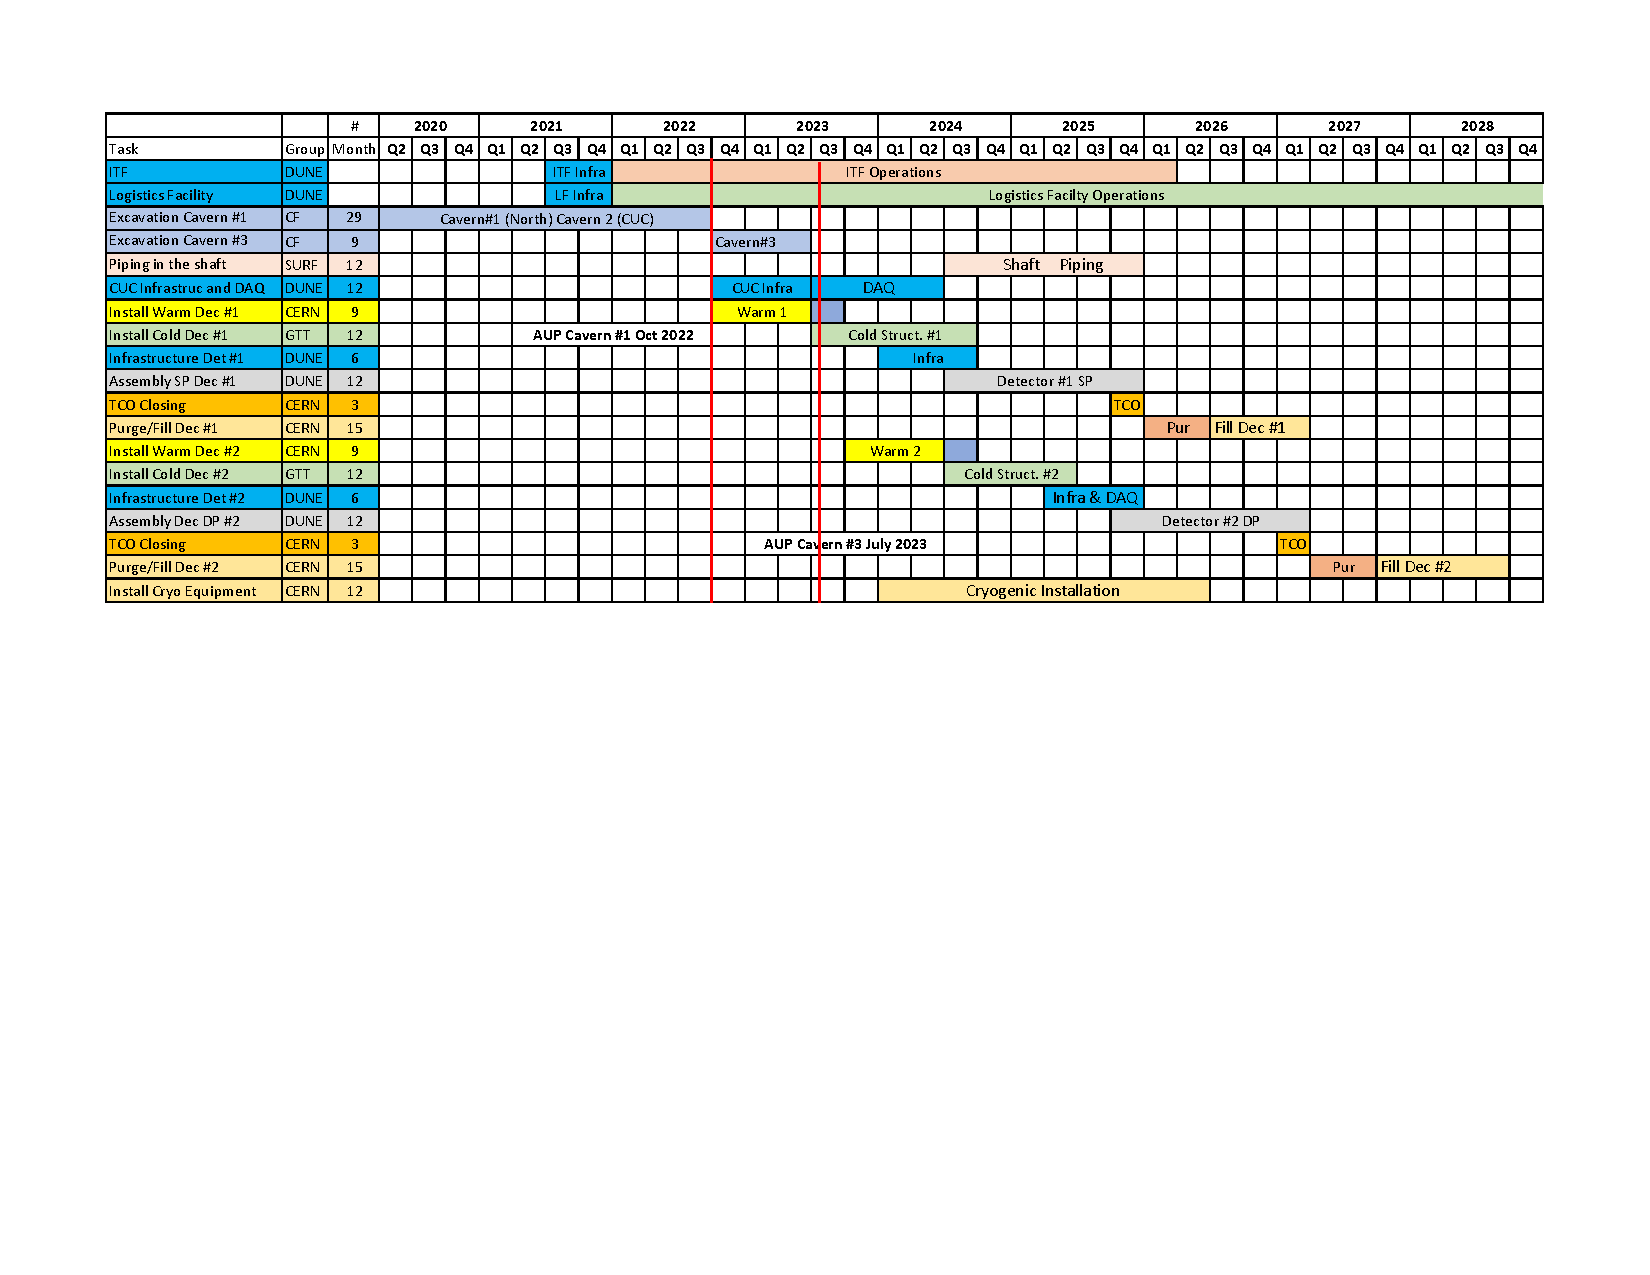
\includegraphics[width=.99\textwidth]{high-level-schedule}
\end{dunefigure}



As mentioned in Section~\ref{sec:fdsp-tc-log}, the \dword{dune} detector installation will proceed in three phases: \dword{cuc} set up, installation set up, and the detector installation. The schedule in Figure~\ref{fig:high-level-schedule} shows the major underground activities and gives an idea of what work occurs in each phase. 

The first phase, \dword{cuc} set up, begins when the underground area for the north cavern and \dword{cuc} become available to \dword{lbnf} and \dword{dune}. At this time, the \dword{lbnf} cryostat construction begins in the north cavern, and \dword{dune} equipment installation 
begins in the \dword{cuc}, specifically, infrastructure in the \dword{dune} data room. Figure~\ref{fig:cavern-layout} shows a top view of the underground areas and the location of the dataroom at the west end of the CUC. 

The detector installation setup phase (referred to as Infrastructure Det\#1 in the table in Figure~\ref{fig:high-level-schedule}) begins during the cryostat membrane installation period. 
In this phase, the equipment needed for detector installation is erected in the north cavern. This includes the bridge across the cavern, the cleanroom, lifting equipment and work platforms, the \coldbox{}es and cryogenics system for \dword{apa} testing, and the \dword{dss} and switchyard. 
The detector itself is installed in the third phase of the installation. 

\begin{dunefigure}[Layout of the DUNE underground areas]{fig:cavern-layout}
  {Top view of the layout at the 4850 level at \dword{surf}. Shown are the three large excavations and the location of detectors in the north (upper) and south caverns. 
  The \dword{cuc} in the middle houses the \dword{dune} data room and the underground utilities.}
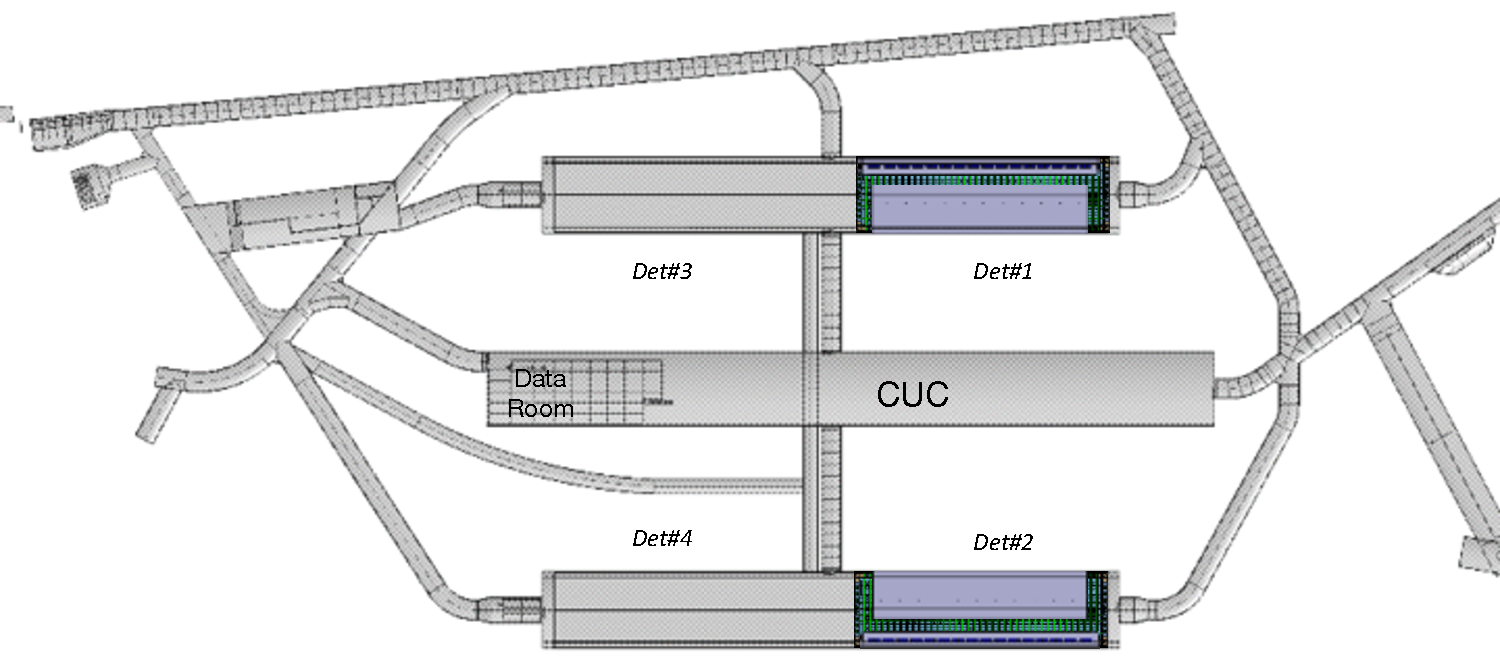
\includegraphics[width=.9\textwidth]{cavern-layout}
\end{dunefigure}


%%%%%%%%%%%%%%%%%%%%%%%%%%%%
\subsection{Installation Process Description}
\label{sec:fdsp-tc-inst-proc}


\subsubsection{CUC Installation Phase}
\label{sec:fdsp-tc-inst-CUC}

\begin{dunefigure}[Layout of the DUNE data room and work area in CUC]{fig:install-cuc}
  {Top: The overall layout of the \dword{dune} spaces in the \dword{cuc}. A110 is the \dword{dune} data room, which houses the underground computing, and A111 is a general-purpose work area (not a control room, as labeled) that we call the experimental work area. Bottom: The first row of ten racks in the data room is shown. The first two represent the \dword{cf} interface racks. The images were taken from the ARUP 90\% design drawings U1-FD-A-108 and U1-FD-T-701.
  \fixme{add reference to arup 90\% BSI -Anne sent email to Kate S 4/24}}
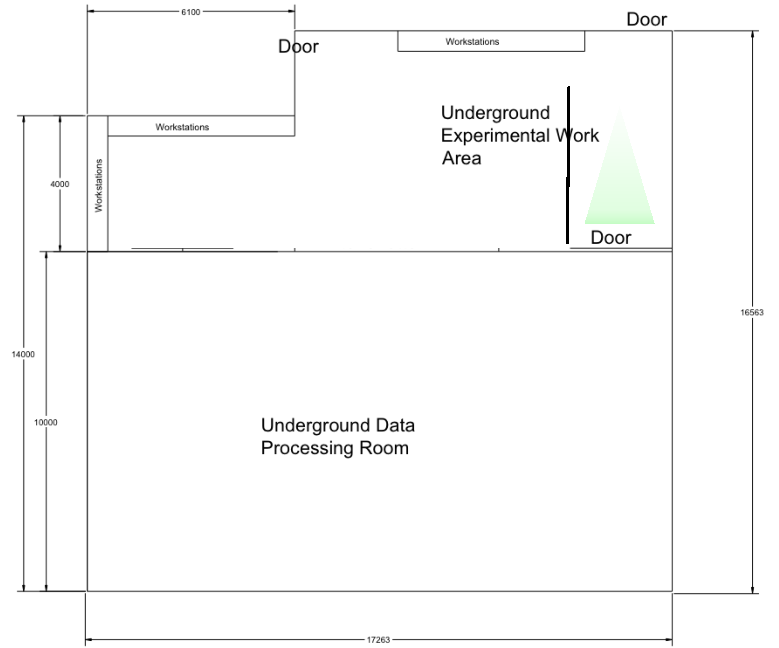
\includegraphics[width=.85\textwidth]{cuc-layout}
\vspace{-2pt}
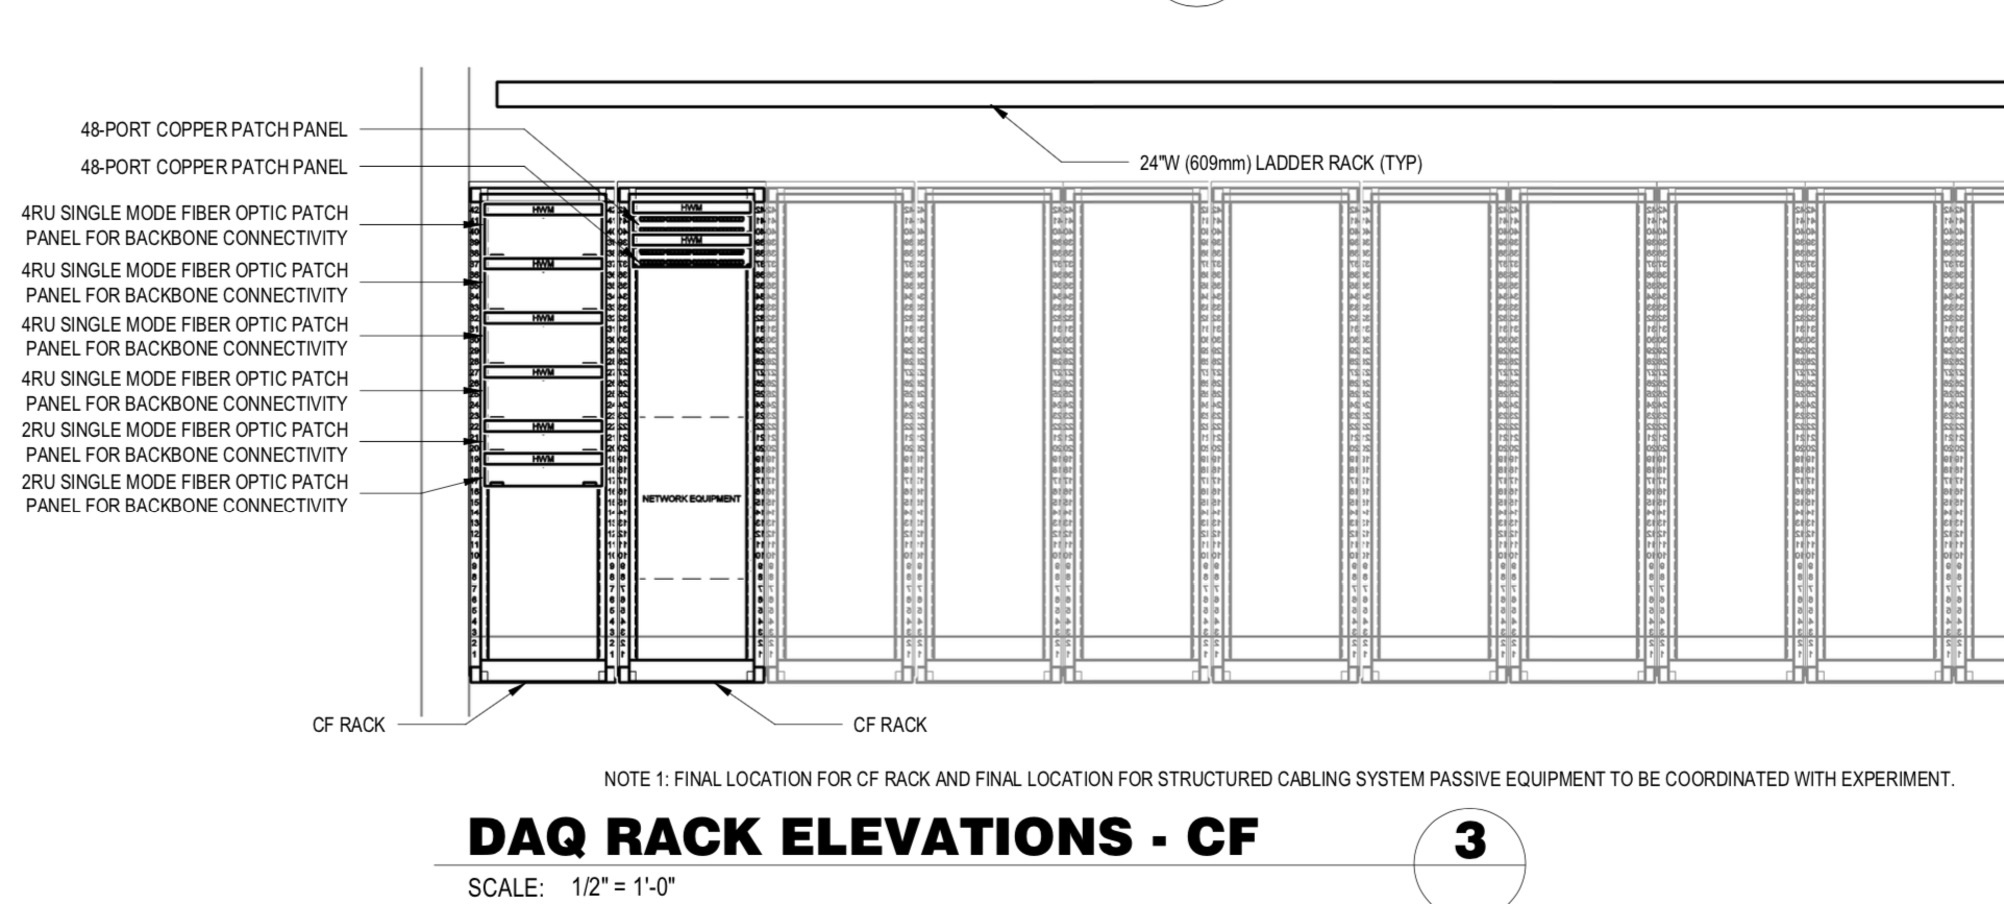
\includegraphics[width=.9\textwidth]{cuc-cf-racks}
\end{dunefigure}

 
Once the \dword{lbnf} \dword{cf} outfitting of the north cavern and the \dword{cuc} is complete,  \dword{lbnf} begins the first cryostat installation in the north cavern and \dword{dune} can begin to install equipment in the data room and work area room in the \dword{cuc}. See Figure~\ref{fig:install-cuc}.  \dword{dune} will not have access to the north cavern due to the heavy steel work for the cryostat. 
At this point \dword{lbnf}  \dword{cf} will have installed redundant single-mode fiber up the shafts to provide external connectivity, and in the empty data room,  an \SI{18}{in} false floor, a \SI{500}{kVA} power disconnect, and connections for sufficient chilled water to cool the racks. The data room, like the adjacent \dword{cf} electronics room, will be outfitted with a dry fire-extinguishing system. 
 

The water-cooled racks, cable trays, power distribution, and water distribution in the data room are the responsibility of \dword{dune} and will be installed once the space becomes available.  
Installation of the racks must be coordinated with \dword{cf} 
since the first two racks are for \dword{cf} use and must be in place before the first phase of work underground is complete. 
Some small overlap will be needed between \dword{cf} and \dword{dune} at this time. The general-purpose network will be installed by \dword{fnal}'s \dword{sdsd} and connected to the Ross Shaft fiber optics. 
This is required for most subsequent work in the underground area.
The \dword{daq} fiber trunk between the detector cavern and the \dword{cuc} data room will be installed after the cable trays, electronics mezzanine, and racks are available in the north cavern.


Data from the detector electronics will be transmitted over a multimode fiber trunk from the \dwords{wib} on top the \dword{spmod} to the \dword{daq} data room in the \dword{cuc}, shown in Figure~\ref{fig:install-cuc}.  The data room will contain 60 water-cooled racks, two of which are reserved for \dword{cf} use, two for \dword{cisc} servers, and the rest for \dword{daq} servers and networking. Racks for all four modules will be installed at the beginning of the \dword{cuc} commissioning phase because they must be plumbed into the cooling water below the data room's drop floor and wired into power distribution from the ceiling.  \dword{daq} equipment will populate the racks as needed for servicing the detector commissioning.  For the first \dword{detmodule}, details of this configuration will be informed by \dword{daq} vertical slice tests done at other institutions.  

At the same time, the eight above-ground \dword{daq} racks that receive data from the underground data room and  transmit the data to \dword{fnal} will %also 
be installed, connected to the WAN, and connected to the single-mode fiber in the Ross and Yates Shafts.  With this infrastructure in place, the \dword{daq} group can begin constructing and testing the final \dword{dune} \dword{daq}, starting with the timing system. 
Enough \dword{daq} back-end servers to support the first \dword{apa}s will be operational before the \dword{apa}s are installed.  The remainder of the \dword{daq} will grow in parallel with \dword{apa} installation.

The underground experimental work area (shown as ``CONTROL ROOM'' in Figure~\ref{fig:install-cuc}) must serve a variety of purposes during the \dword{dune} installation. Initially, the area will be outfitted with office equipment for the installation team, workstations for \dword{daq}, and a basic conference area for meetings. The room is \SI{17}{m} wide with portions that are \SI{5.5}{m} and \SI{8}{m} deep.

During this early installation stage, the machine shop and \dword{dune} storage area will be set up in the detector excavation area and shared with the cryostat team. 

\subsubsection{Installation Setup Phase}
\label{sec:fdsp-tc-inst-setup}

\begin{dunefigure}[Top view of the installation area highlighting the infrastructure]{fig:install-infrastructure-top}
  {Top view of the installation area highlighting the infrastructure. The cleanroom roof and cavern walls are removed in this view.}
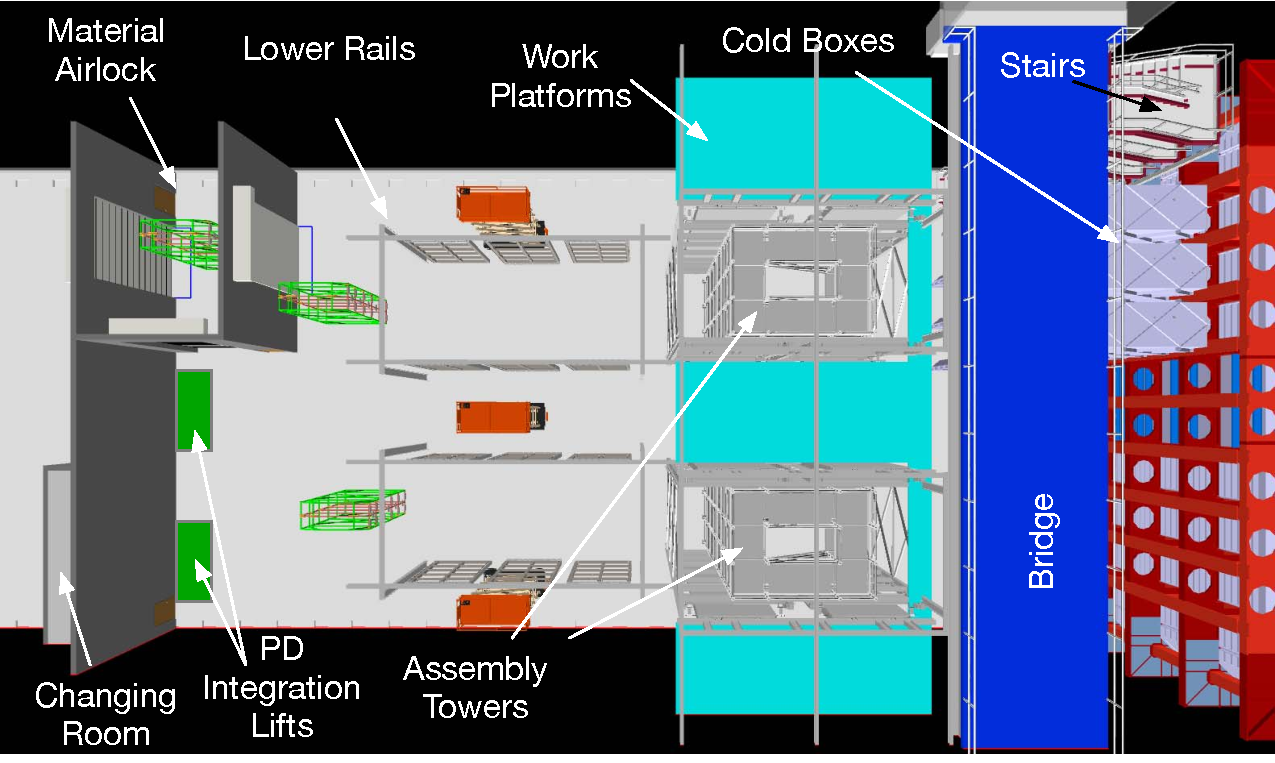
\includegraphics[width=.85\textwidth]{install-infrastructure-top}
\end{dunefigure}

Once the steel structure of the cryostat is complete, the remaining work by the \dword{lbnf} cryostat team will be focused inside the cryostat installing the insulation and membrane.  
\dword{lbnf} activity outside the cryostat will consist mainly of
transporting the 4,000 crates of foam and other materials from the cavern to inside the cryostat. 
Since the cryostat outer steel structure will be in position, \dword{dune} can 
begin installing the infrastructure needed to install the detector outside the cryostat. 
Figure~\ref{fig:install-infrastructure-top} shows the major pieces of infrastructure supporting the detector installation.
The first piece of equipment is the bridge between the north and south drifts. 
This will allow the cryogenics equipment to travel from the north drift to the \dword{cuc} and will provide part of the structure for the cleanroom. It also provides an additional means of egress in an emergency. \fixme{printing error occurs here (Gina found)}

As part of the bridge construction, the crane under the bridge will be mounted. This 
will be used to lift crates off the floor and bring them into the cryostat, freeing the cavern crane for work elsewhere. The decking on top of the cryostat is also installed in this early stage to provide a safe work surface. 

The largest and most time-consuming pieces of equipment to  construct in this phase are the three \coldbox{}es and their associated cryogenics system. 
The \coldbox{}es, visible in Figures~\ref{fig:install-coldbox} and \ref{fig:install-infrastructure-top}, will likely need to be constructed in place due to their size (see Section~\ref{sec:fdsp-tc-infr-cryo}) and fabrication will begin as early as possible.  
If it is possible to bring them down the shaft partially assembled, then once the first \dword{detmodule} is complete, we can break them down to their pre-assembled parts and move them to the second \dword{detmodule} area.

 
After the bridge crane under the north-south bridge is in place the \dword{apa} assembly and cabling towers are installed. 
The two towers have enough space between them, as described in Section~\ref{sec:fdsp-tc-infr-comm}, to walk through or work. 
With the towers in place the north-south support beams and the fixed platforms can be installed. 
This work is done at height so it will only cause temporary interruptions to the material transport along the floor to the cryostat; the lower set of rails and the \dword{cpa} assembly equipment be installed at the convenience of the cryostat installation crew.

When the cryostat membrane work is complete the cryogenic piping inside the cryostat can be installed, the cryostat cleaned and the false floor installed. After the cryostat is cleaned the HEPA filters will be installed in air handling units for the cryostat and purified air will begin flowing. A curtain over the \dword{tco} can be used to prevent dust from the cavern from entering the cryostat until the cleanroom walls are constructed.

In parallel to the installation of the cryogenic piping the walls of the cleanroom can be assembled and AC power and fire suppression installed. Finally the floor is painted and 
cleaned, then the cleanroom is ready for operation.



On the cryostat roof the installation of the cryostat crossing tubes proceeds in parallel to the cryostat membrane assembly sequence.  \fixme{add LBNF TDR reference. } 
\fixme{The crossing tubes are welded to the membrane on the inside so they are installed as the membrane is installed.}
The crossing tubes are welded to the \SI{1}{cm} thick steel cryostat roof and cross braced to the large I-beams. 
The thin-walled tubes that penetrate the foam insulation are welded to the cryostat inner membrane.


\begin{dunefigure}[Installation of electronics crosses]{fig:install-elect-cross}
  {Installation of the crosses to which the \dword{tpc} electronics warm readout and the \dword{pd} cables are connected.
  }
 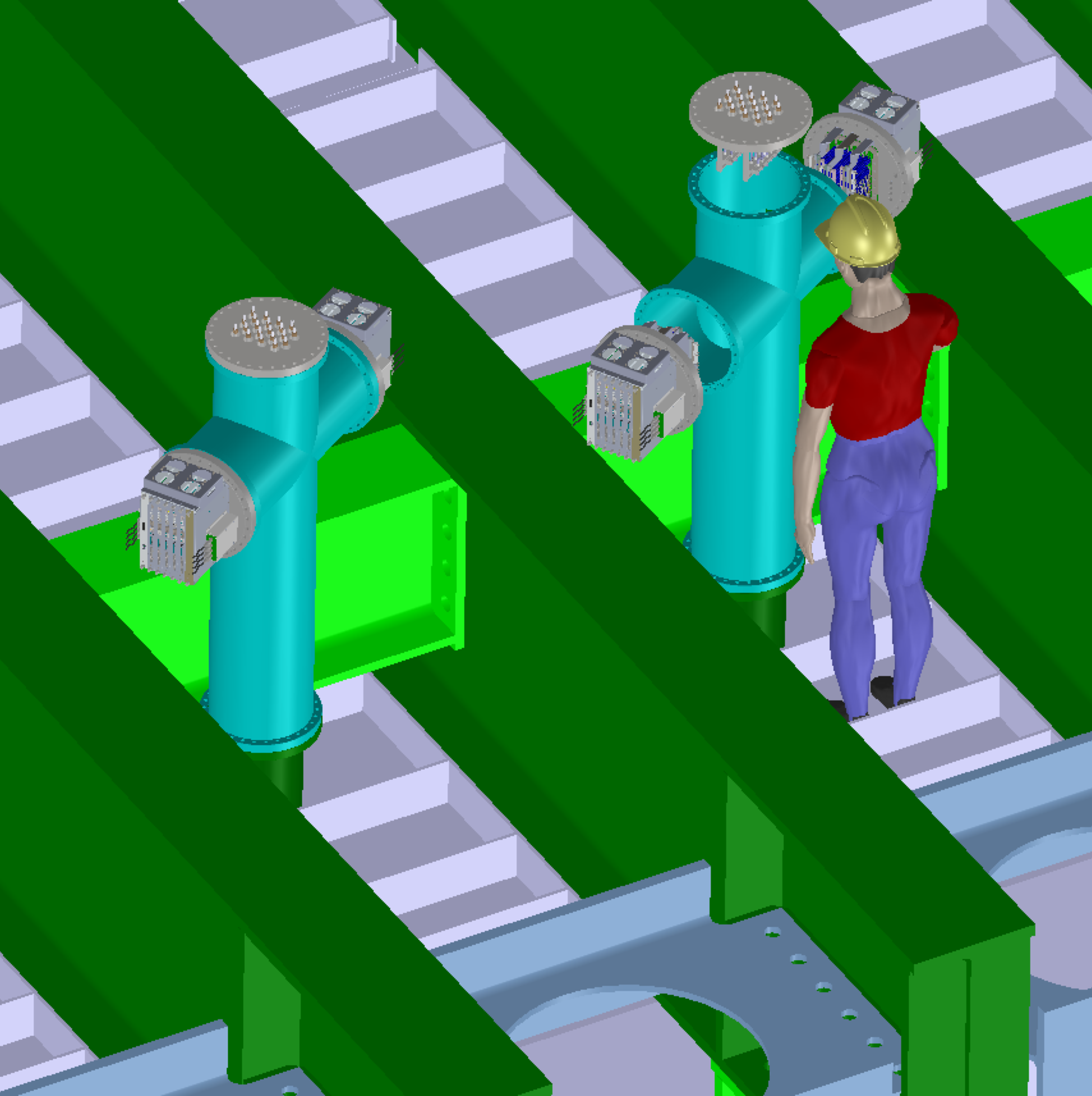
\includegraphics[width=.5\textwidth]{install-elect-cross}
\end{dunefigure}



Once the crossing tubes are installed and leak-chased, we connect the  \dword{tpc} electronics crosses and mount  the  \fdth flanges for the \dword{ce} and \dwords{pd} onto the crosses. 
The height of the crosses was chosen to allow a person to work comfortably on the \dwords{wiec}  and \dword{pd} flanges while standing on the cryostat roof. 
A fully assembled cross is shown on the left of Figure~\ref{fig:install-elect-cross}, and a cross with a \dword{wiec} extracted in ``assembly position'' is shown on the right. 
The present plan is to install the crosses shortly after the cryostat crossing tubes are installed. 
This allows us to seal the large openings in the cryostat roof to prevent dust from entering.
For this stage, temporary rubber seals are used for the flanges because they must be removed during the cabling process later in the installation. 
When the \dword{wiec} installation is complete the \dword{tpc} electronics is ready for the installation of power and fiber optics for readout. 

\begin{dunefigure}[DSS \fdth  installation]{fig:install-dss-feedthru}
  {The \dword{dss} support \fdth{}s  are installed using a gantry crane running along the roof of the cryostat.
  The cryostat decking is not shown. 
  The gantry can move freely on the cryostat roof decking. The gantry crane is selected to fit under the mezzanine as shown in the right panel.
  }
  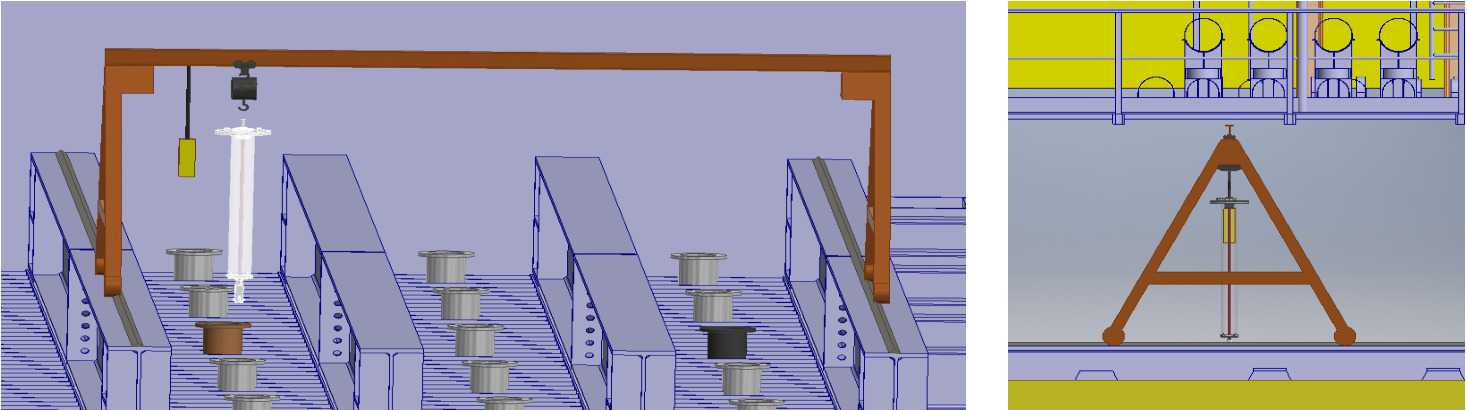
\includegraphics[width=.98\textwidth]{graphics/install-dss-feedthru-v2.pdf}
\end{dunefigure}


The \dword{dss} support \fdth{}s can be installed in parallel to the \dword{tpc} electronics crosses. This is the first step in the \dword{dss} installation. 
A gantry crane on top of the cryostat picks up the \fdth{}s  and lowers them into the cryostat crossing tubes as shown in Figure~\ref{fig:install-dss-feedthru}. 
There are \num{20} \fdth{}s per row and five rows, for a total of \num{100} \fdth{}s.  A fixture with a tooling ball is attached to the clevis of each \fdth{}.  
The horizontal $XY$ and the vertical $Z$ positions of this tooling ball are defined, a survey is performed to determine the location of each tooling ball center, and adjustments are made to get the tooling ball centers to within $\pm$\SI{3}{mm} of the nominal position.  
The \SI{6.4}{m} long I-beams are then raised and pinned to the clevis.  
Each beam weighs roughly \SI{160}{kg} (\SI{350}{lbs}). 
A lifting tripod is placed over each  \fdth{}'s supporting beam, and a \SI{0.64}{cm} (\SI{0.25}{in})  cable is fed through the top flange of the \fdth down \SI{14}{m} to the cryostat floor where it is attached to the I-beam. 
The cable access port and lifting cable are shown in Figure~\ref{fig:dss-beam-lifting}. 
The winches on each tripod raise the beam in unison to position it at the correct height for pinning to the \fdth clevis.  Once the beams are mounted, a final survey of the beams ensures proper placement and alignment. 
 \begin{dunefigure}[DSS I-Beam lifting setup]{fig:dss-beam-lifting}
  {A cable access port is included in the \dword{dss} flange. This is used to feed a cable from the roof through the flange and attach it to the I-beams during \dword{dss} installation.}
 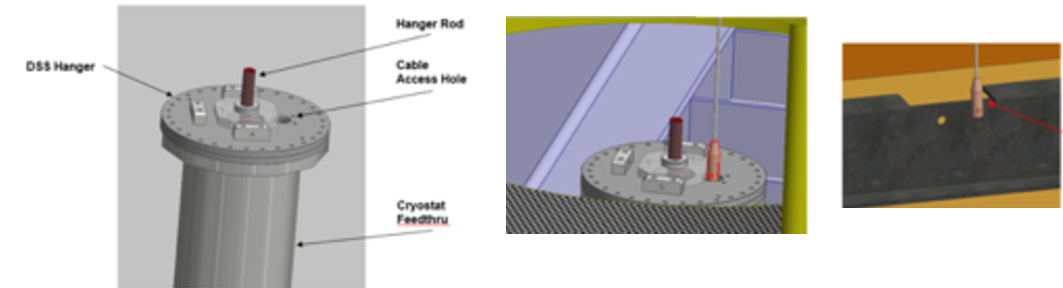
\includegraphics[width=.95\textwidth]{graphics/dss-beam-lifting.pdf}
\end{dunefigure}


Next it is time to install the mezzanines for the cryogenics system and the detector electronics racks, followed by the cable trays,  piping, lighting, and cryostat roof flooring. At this point, the cryostat roof is ready for \dword{daq} and cryogenic system installations to begin; this will proceed in parallel with the detector installation.





\subsubsection{Detector Installation Phase}
\label{sec:fdsp-tc-inst-execute}



At the start of the detector installation phase, the cleanroom and all equipment inside are operational, the \dword{dss} is installed, and the cryostat is clean and ready for installation. 
Figure~\ref{fig:install-infrastructure-top} shows the layout (plan view with the roof removed) of the cleanroom during the detector installation phase; the cryostat is on the right and the open cavern on the left. 
In the north-east corner of the figure (upper right corner), the access  (permanent) stairway is shown. 
This stairway is inside the cleanroom and allows people easy access to both the work platforms and the cleanroom floor. 
The doors to the stairway will never be locked; the stairway is considered a means of egress in emergency, as it leads to an exit through the mucking drift.
A second stairway and an industrial elevator at the west entrance to the cavern provide access to the cavern floor for personnel and equipment. 
The primary changing room is in the southwest corner of the cleanroom and a smaller changing room (shown in Figure \ref{fig:install-cleanroom}) will be situated near the stairs at the 4850 level for people accessing the work platforms.

In the north-west corner of the cleanroom is the material airlock where all materials enter  through tall doors. 
Outfitting the airlock with a removable roof is under consideration. 
It would allow entry of equipment via the cavern crane, which could facilitate the process.
 
Labor for the detector installation phase is split between the \dword{jpo} and the \dword{dune} consortia. 

The \dword{jpo} labor includes a scientific lead, a manager, two deputy managers (one manager on each shift), three safety officers (one on each shift), and administrative help. They are responsible for communicating with the logistics organization to ensure needed components are shipped underground and properly maintained in the inventory system.  
They also organize and plan daily the underground tasks with the lead workers and rigging teams, as well as with the different consortia.  
Several teams of three \dwords{fte} from the \dword{jpo}, consisting of a lead worker and riggers, are responsible for moving all detector components into the materials airlock,  cleanroom, \coldbox (if needed), and cryostat. 
An additional team (lead worker, riggers and technicians) works in the cryostat to position the \dword{tpc} components and, during the final stage of each new drift volume,  deploy the \dwords{fc}. 
\fixme{check prev pgraph against vol 5 when ready. anne}

Each of the \dword{dune} \dword{fd} consortia has specific tasks related to its subsystem. 
The installation activities are planned estimating both the \dword{jpo} and consortia labor contributions.

\begin{dunefigure}[Design of the instrumentation \fdth{}s feedthroughs]{fig:CISC-feedthru}
{Design of the instrumentation \fdth{}s feedthroughs. The signal \fdth is integrated with the \dword{dss} support \fdth{}s. A side port on a short spool piece in the \dword{dss} support structure allows the instrumentation cables to be fed through the cryostat walls where needed.}
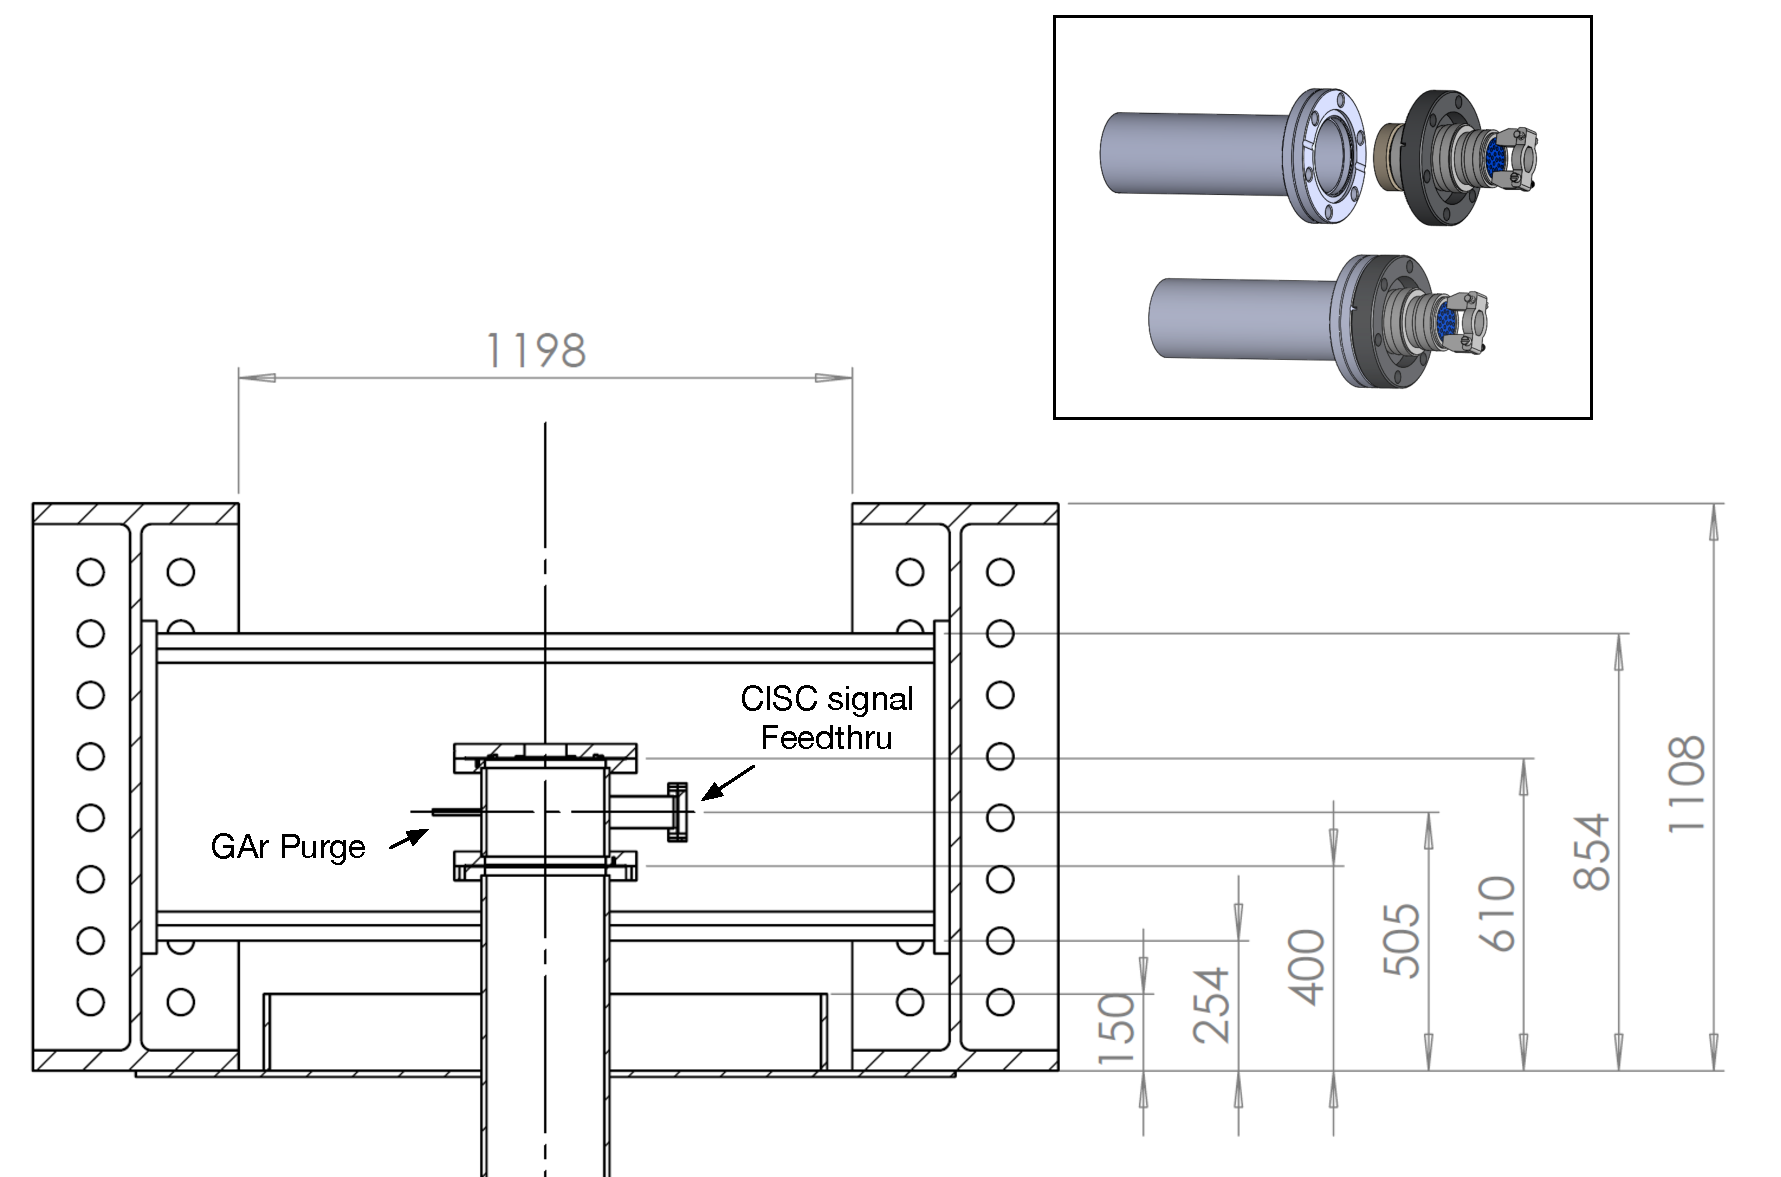
\includegraphics[width=0.95\textwidth]{CISC-feedthru.pdf}
\end{dunefigure}

The first detector equipment to be installed are \dword{cisc} T-gradient thermometers, an array of purity monitors, and cameras, all at the east end of the cryostat. This equipment will be used to monitor the \cooldown, filling, and commissioning of the detector. Some equipment for the laser calibration system is also installed at this time, including some positioning diodes and possibly an optical mirror-based switching system.  The signals exit the cryostat via electrical \fdth{}s distributed across the cryostat roof and integrated with the \dword{dss} support structure, as shown in Figure~\ref{fig:CISC-feedthru}. Because all these components are small, they can be installed using a scissor lift with \SI{12}{m} reach. At present, this is the tallest battery operated (thus cleanroom compatible) scissor lift rated for use in the USA that we have identified.



Cabling for the remaining static T-gradient monitors is also installed before the start of \dword{tpc} installation.  The thermometer cables and mechanical supports are anchored to the cryostat using the bolts running along the cryostat's top and bottom edges and can be installed once the cryostat is clean. 
To avoid  damaging the small and fragile thermometers, they are not plugged into the small IDC-4 connectors until just before the corresponding \dword{apa} is moved into its final position. 
Cables and supports for the thermometers on the pipes below the detector and on the cryostat floor are installed immediately after installing the static T-gradient monitors on the walls.  
Again, the thermal sensors themselves are installed later, just before unfolding the bottom \dwords{gp}, to avoid damage.

Individual sensors on the top \dword{gp} must be integrated with the other \dwords{gp}. For each \dword{cpa} (with its corresponding four \dword{gp} modules), cable and sensor supports will be anchored to the \dword{gp} threaded rods. Once the \dword{cpa} is moved into its final position and its top \dwords{gp} are ready to be unfolded, sensors on these \dwords{gp} are installed.

 
Installing fixed cameras is, in principle, simple but involves a large number of interfaces. The enclosure for each camera has exterior threaded holes to facilitate its mounting %the camera 
on the cryostat wall, cryogenic internal piping, or \dword{dss}. Each enclosure is attached to a gas line to maintain appropriate underpressure in the fill gas, requiring an interface with cryogenic internal piping. Camera cables are run through cable trays to flanges on assigned instrumentation \fdth{}s. 


A summary of all the cryogenics instrumentation provided by the \dword{cisc} consortium is shown in Figure~\ref{fig:cisc_devices}. 

At this point the quartz optical fibers required for the \dword{pd} monitoring system are run from the optical flange locations (still being finalized) to locations on the \dword{cpa} support beams of the \dword{dss}, to be connected later to the diffusers mounted on the \dword{cpa}s.


The residual gas analyzers that monitor impurities in the \dword{gar} system must be installed before the piston purge and gas recirculation phases of cryostat commissioning.  However the actual installation time depends on the schedule for outfitting the mezzanine and installing the  \dword{gar} purge piping. These  instruments are installed near the tubing switchyard to minimize tubing run length and for convenience when switching the sampling points and gas analyzers. 

\begin{dunefigure}[Distribution of various CISC devices inside the cryostat.]{fig:cisc_devices}
  {Distribution of various \dword{cisc} devices inside the cryostat.
  }
  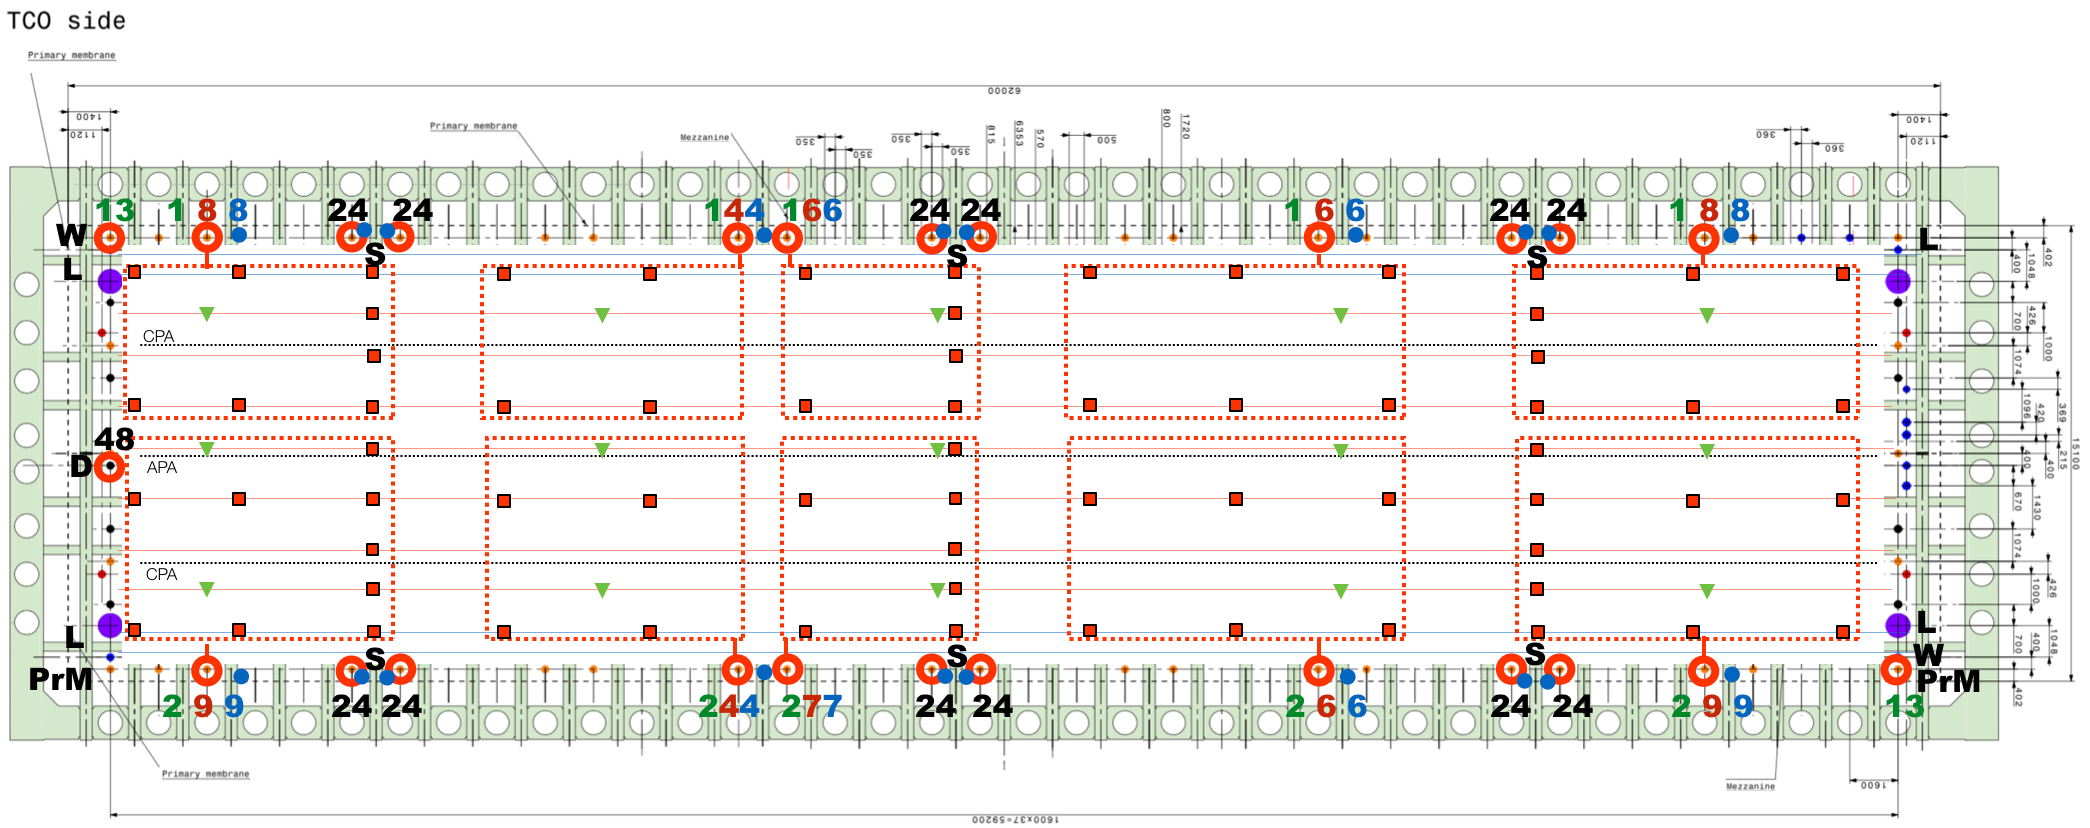
\includegraphics[width=0.98\textwidth]{cisc_distribution.png}
  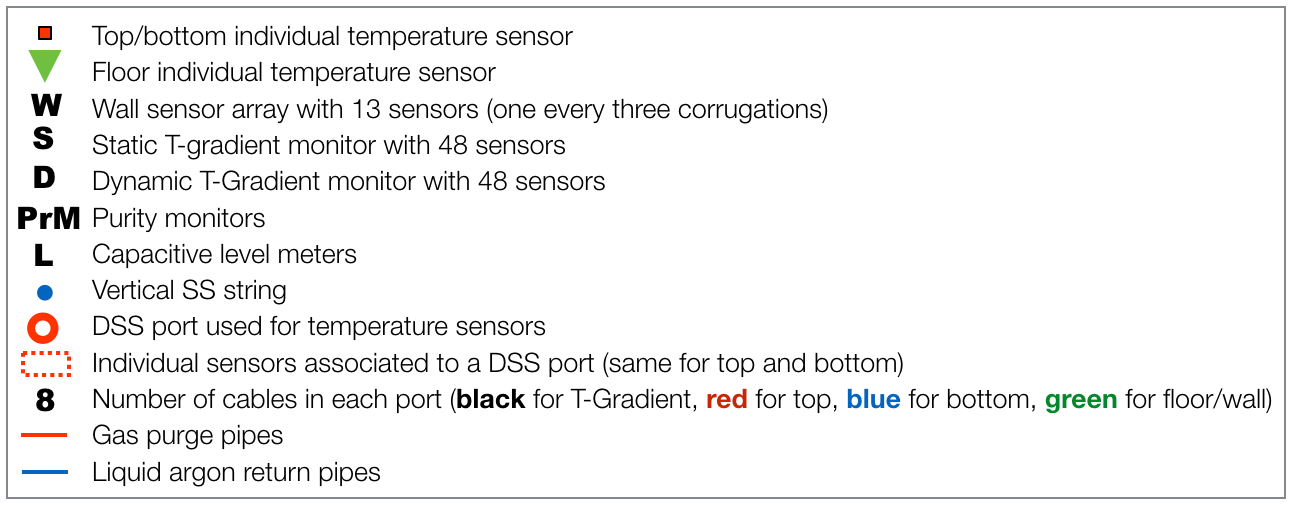
\includegraphics[width=0.85\textwidth]{cisc_distribution_legend.png}
\end{dunefigure}

% clear the figure buffer before starting the next section
\clearpage



Next the east \dword{ewfc} is installed. The endwall planes are brought underground in custom crates. Each of the eight crates holds four endwall modules.  Eight modules are needed to build one complete \SI{12}{m} tall plane.  First a custom hoist is installed on the end of the \dword{dss} beam for lifting and assembling the modules in place, as shown in Figure~\ref{fig:endwall-hoist}. The \dword{ewfc} transport crates are then brought to the material airlock using a forklift where they are cleaned.  Once clean, the crates are moved into the cleanroom and placed next to the \dword{tco}. Then a hoist running on the rails through the \dword{tco} lifts the endwall modules onto the transport cart, which is then hoisted into the cryostat. Figure~\ref{fig:endwall-cart} shows an endwall module being transferred to the transport cart. The top endwall module is then attached to the installation hoist and lifted out of the cart. When the module is free of  the cart, the cart is re-positioned so the second module can be attached to the first, and the pair is then lifted. This process is repeated until the full \SI{12}{m} \dword{ewfc} plane is assembled and can be attached to the \dword{dss}. 
Figure~\ref{fig:endwall-hoist} shows an endwall plane being lifted into position.
All the \dword{hv} connections inside the plane can now be tested. The process is then repeated for the remaining three endwall planes comprising the east  \dword{ewfc}. 
 
 \begin{dunefigure}[Endwall hoisting infrastructure]{fig:endwall-hoist}
  {Image showing the hoisting equipment used to lift the endwall into position. In this image, one of the endwall plane is in place and a second is being positioned. The field shaping strips are not shown.}
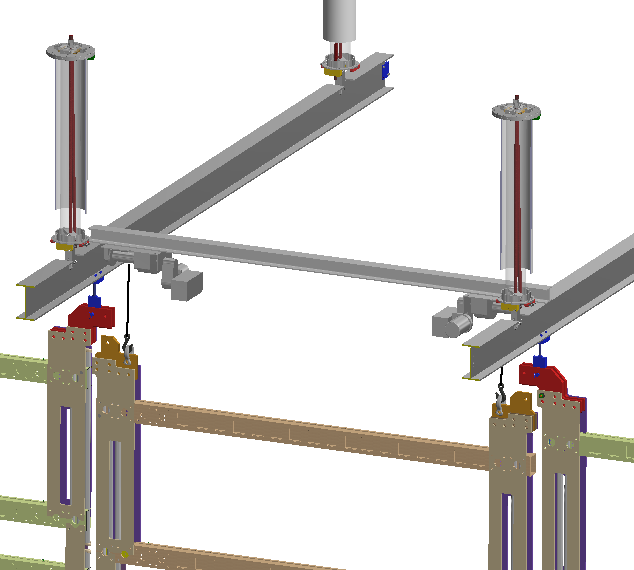
\includegraphics[width=.5\textwidth]{graphics/endwall-hoist.png}
\end{dunefigure}
 
\begin{dunefigure}[Installation of the first endwall]{fig:endwall-cart}
  {The endwalls are lifted out of the transport crates using the one of the hoists on the installation switchyard. Each module is then placed on a custom cart that is lifted into the cleanroom.}
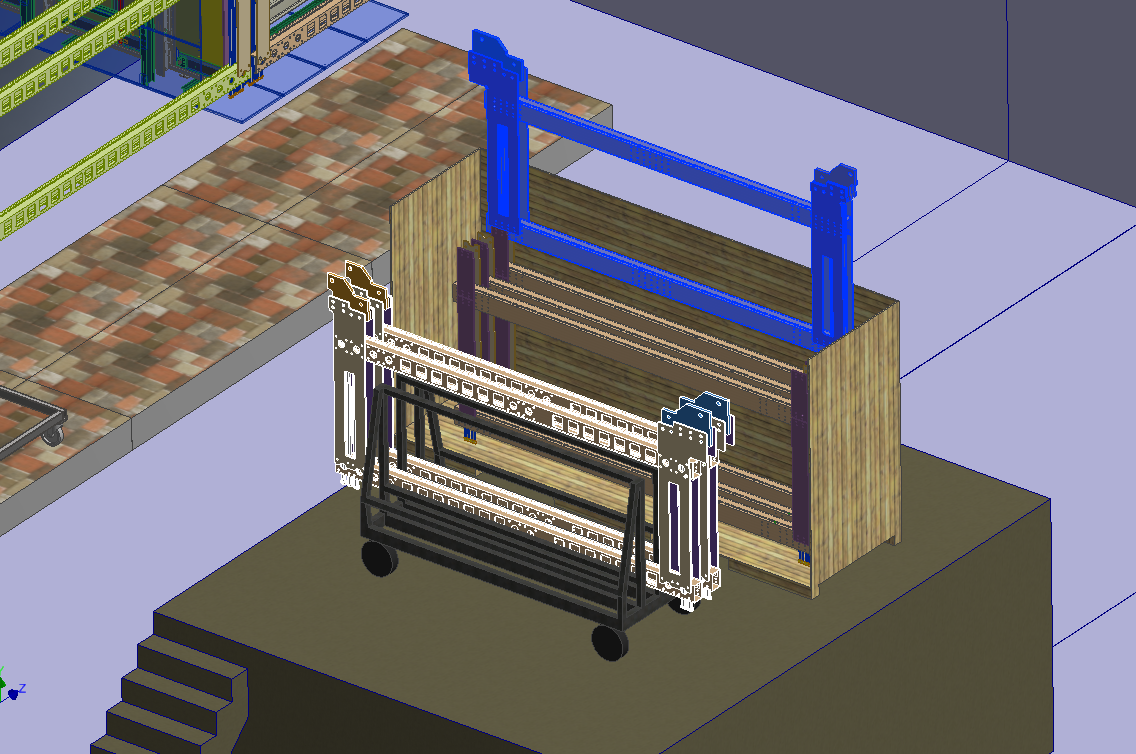
\includegraphics[width=.5\textwidth]{graphics/endwall-cart.png}
\end{dunefigure}




The installation of an \dword{apa} and  \dword{cpa} with top and bottom \dword{fc} modules is the most labor-intensive part of the detector installation. Figure~\ref{fig:install-single-row} represents one of the 25 rows of \dword{tpc}.  \dword{dune} aims to perform work in parallel to the extent possible and finish installing one row every week. 
This requires that several separate teams work in the cleanroom, inside the cryostat, and on the cryostat roof simultaneously --  positioning the equipment, integrating \dword{pd} into the \dword{apa}, mounting the \dword{ce} \dword{femb} on the \dword{apa} connecting the cables, cold testing \dword{apa}, installing \dword{apa} in the cryostat, assembling and installing \dword{cpa}-\dword{fc} and deploying the \dwords{fc}.
Figure~\ref{fig:Single-APA-Schedule} shows the labor breakdown and activities in the airlock,  cleanroom, and cryostat for the \dword{apa} installation. These labor estimates will be refined during time and motion studies at Ash River. 
This complicated installation process will be described in steps: first the \dword{apa} assembly work in the cleanroom, followed by the \dword{cpa} assembly, and finally the installation process inside the cryostat.

While the \dword{apa}s, \dword{cpa}, and \dword{fc} are installed, the area outside the cleanroom in the north cavern is available for storage; this area has sufficient capacity to store one full month's worth of equipment. As it is called for, equipment will be brought into the cleanroom's materials airlock through a roll-up or curtain door in the west wall using either an electric forklift or electric pallet jacks.

\begin{dunefigure}[Single row of APA and CPA]{fig:install-single-row}
{One row of the \dword{apa} and \dword{cpa} with associated \dwords{fc}. The \dwords{fc} are shown deployed in the final orientation. The equipment in the figure represents $1/25$ of the total \dword{tpc}.}
 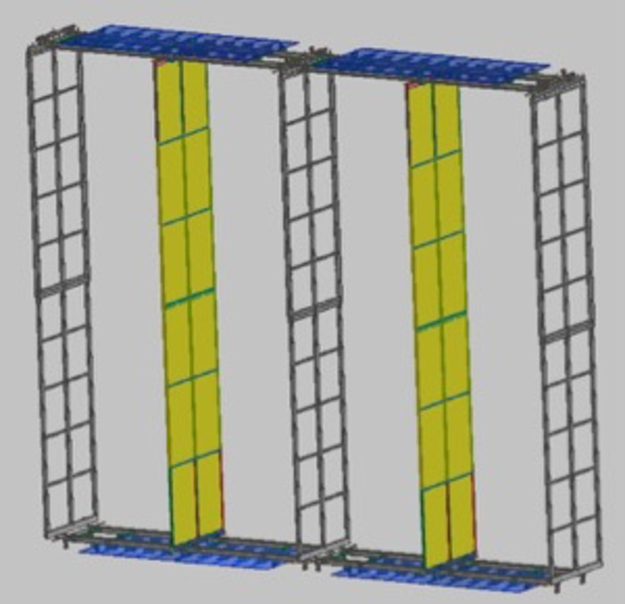
\includegraphics[width=0.3\textwidth]{install-single-row}
\end{dunefigure}

\begin{dunefigure}[Typical APA installation schedule]
{fig:Single-APA-Schedule}
{Typical \dword{apa} schedule for \dword{spmod}}
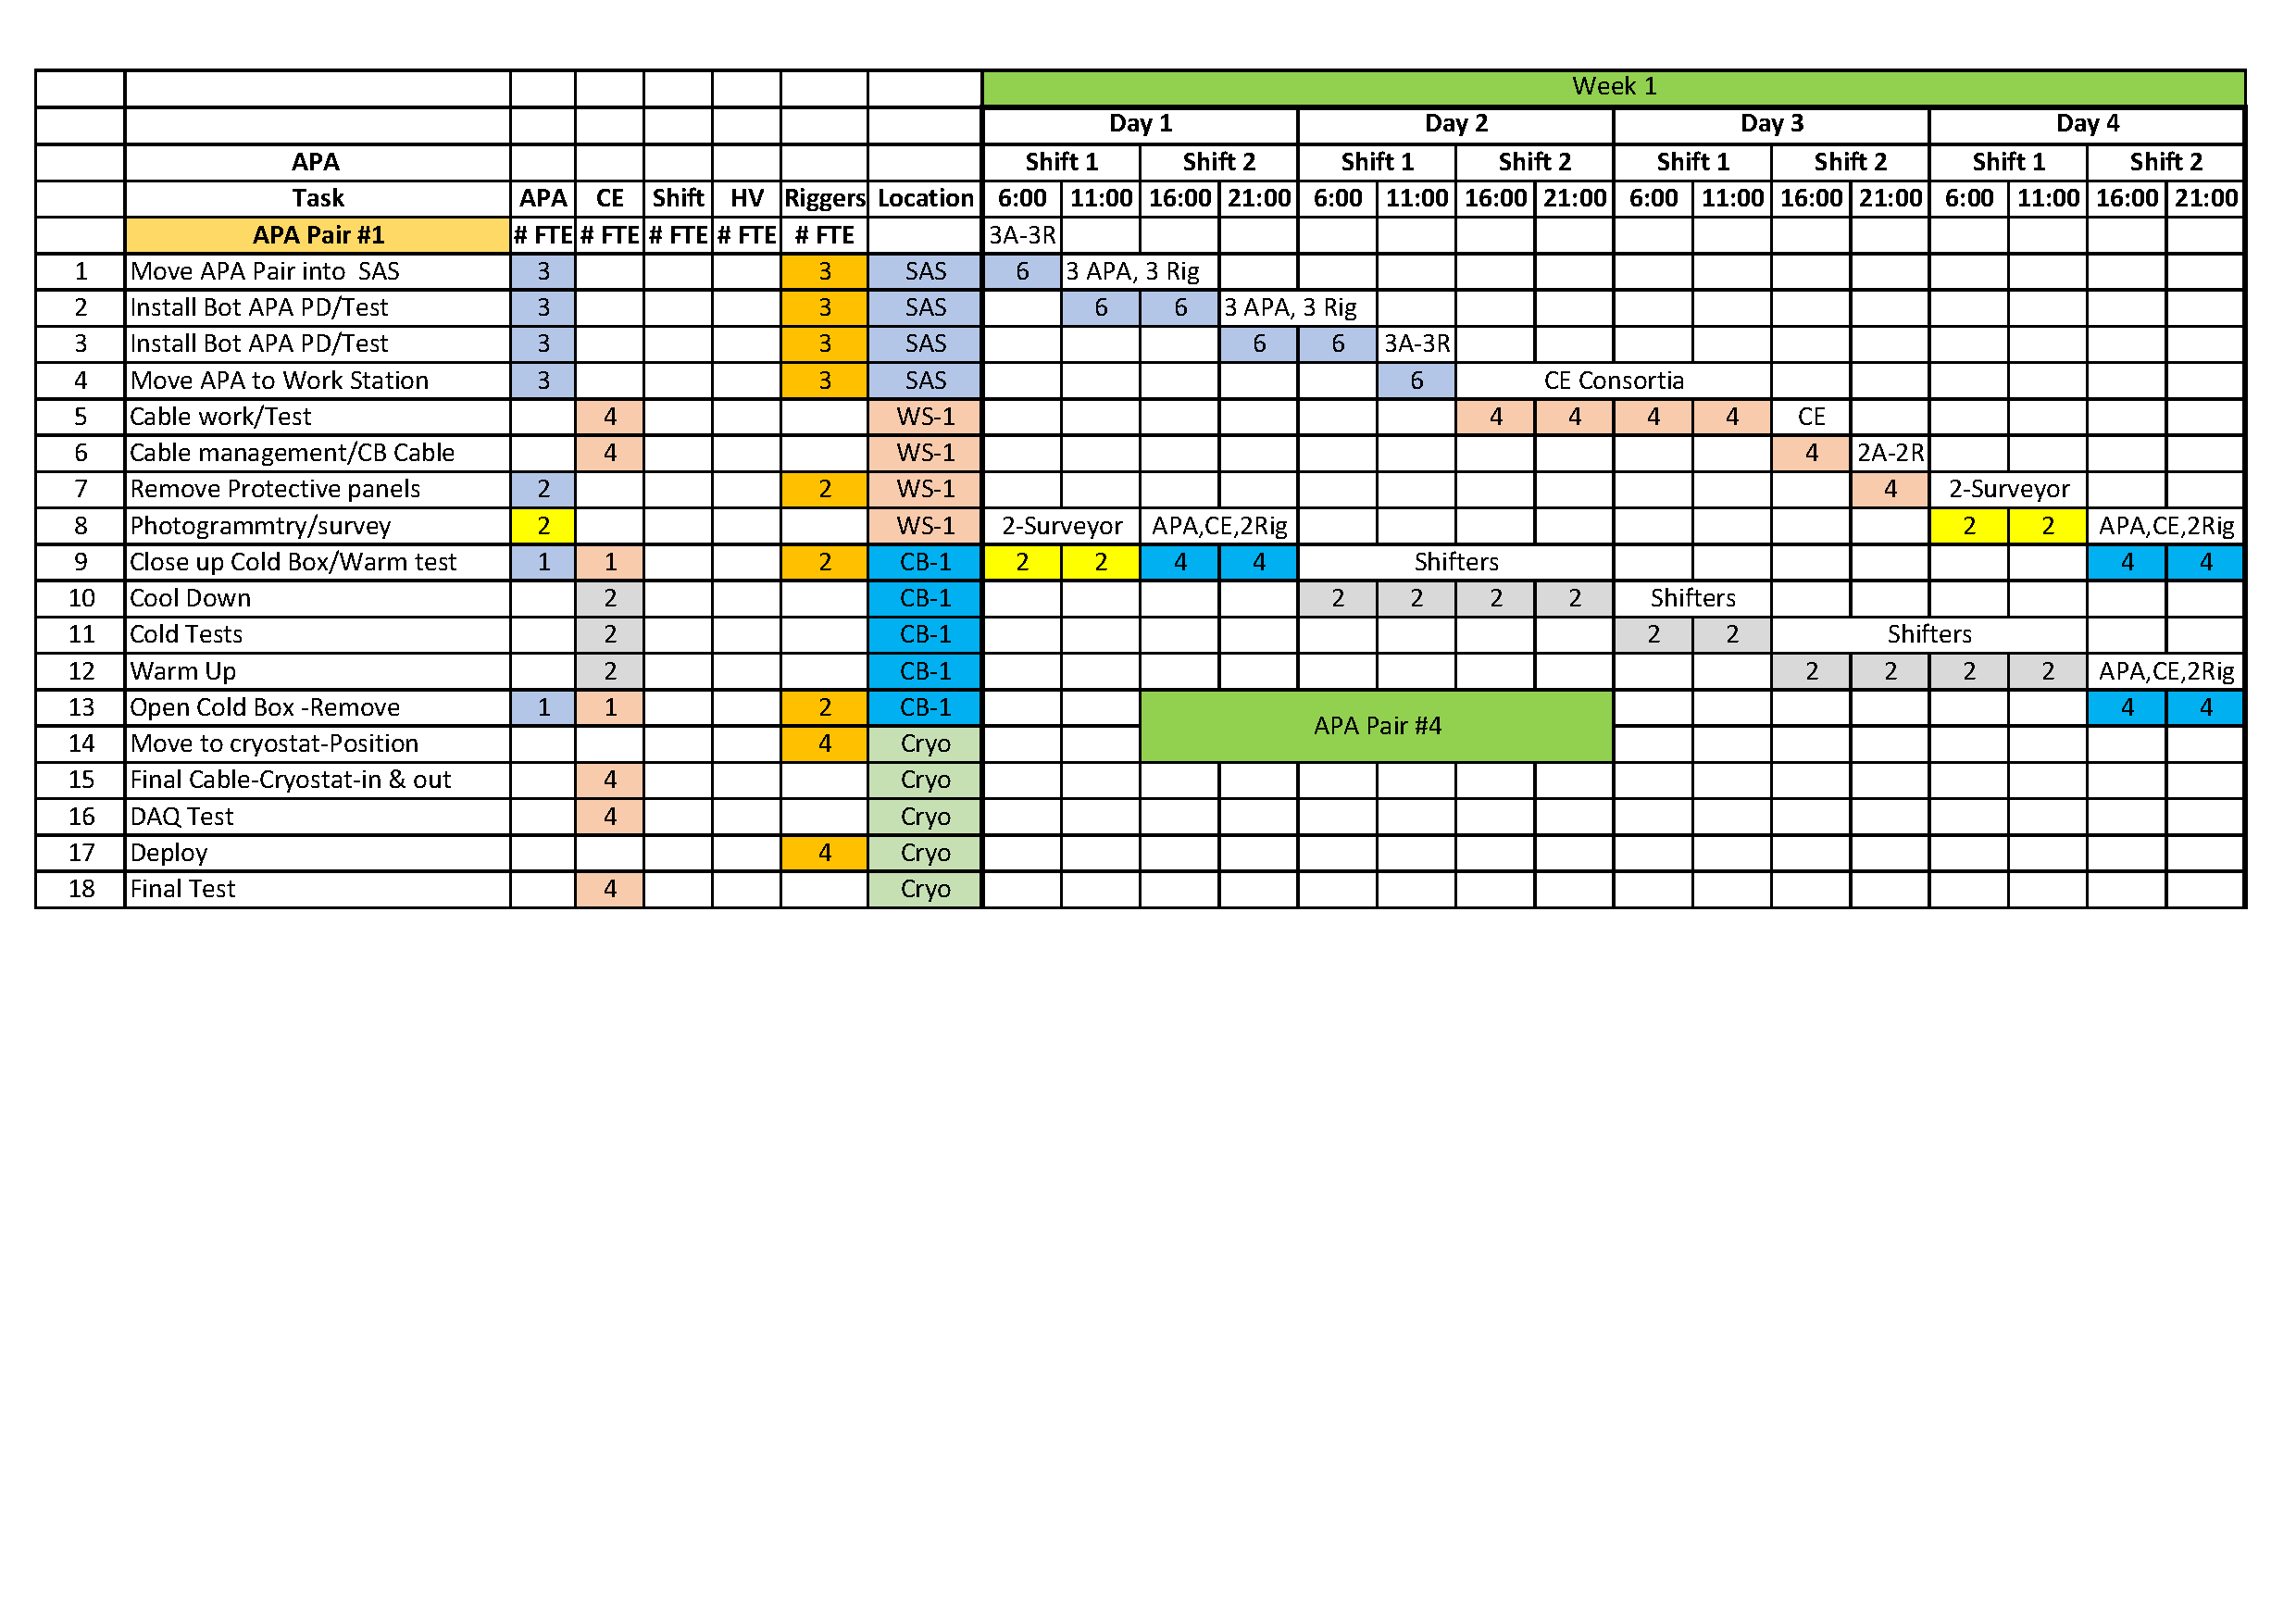
\includegraphics[width=0.95\textwidth]{Single-APA-Schedule.pdf}
\end{dunefigure}


  
An \dword{apa} transport crate that holds two \dword{apa}s  is first rotated to the vertical orientation and bolted to a custom-weighted skid or cart used for moving the crate in the cleanroom. 
Battery powered pallet jacks move the crate into the materials airlock where the outer covers are removed and the outer frame cleaned. 
After the air purity has recovered, the transport box can be brought into the cleanroom proper. 
The \dword{apa}s are first moved to the \dword{pd} integration area where the \dwords{pd} are inserted into the sides of the \dword{apa}. 
The \dword{apa} transport boxes and \dword{apa} protective covers are designed to keep the slots in the sides for the \dwords{pd} clear. 
The \dword{apa} transport box is placed between two fixed scissor lifts. The transport box is situated so that two-person teams in the lifts can easily hold a \dword{pd} module on the side of the lift. 
The lift is raised to align the paddle with one of the five slots in the side of the \dword{apa}. The paddle can then slide into the side of the \dword{apa}. 
The guides inside the \dword{apa} frame ensure that the electrical connectors in the middle of the \dword{apa} mate easily. 
The \dwords{pd} are locked in position with two captured screws. 
After each \dword{pd} is installed it can be tested electrically by accessing the connectors at the top using a scissor lift. 
Once the ten \dword{pd} paddles are installed on the first \dword{apa}, the transport crate is shifted slightly and the \dwords{pd} can be inserted into the second \dword{apa} and tested. 
The \dword{apa} transport crate may need to come out from between the lifts to install the lower \dword{pd} modules.

\begin{dunefigure}[Photon detector and APA integration]
{fig:install-pd-integrate}
{Area where the \dwords{pd} are integrated into the \dword{apa} modules. Floor-mounted scissor lifts are used to access the sides of the \dword{apa}.}
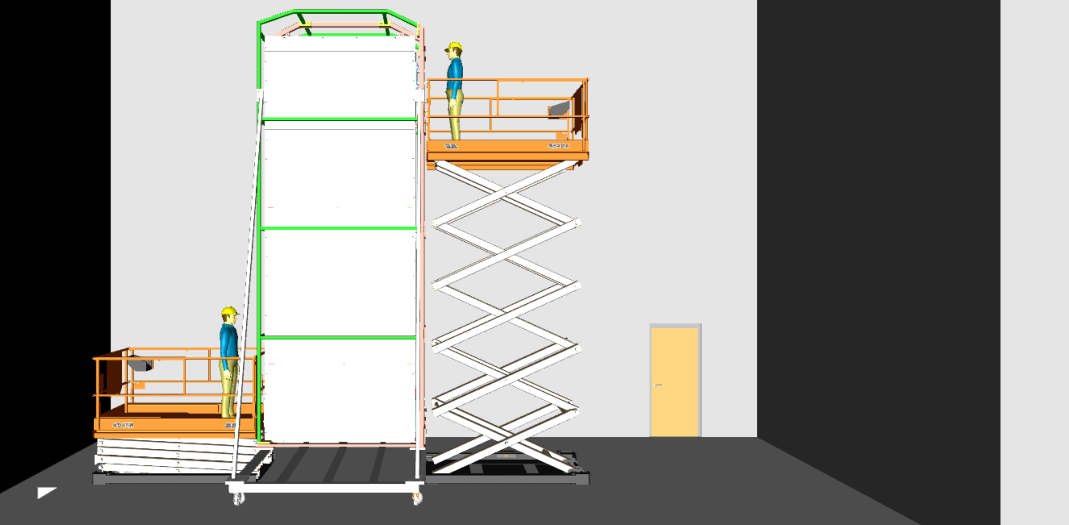
\includegraphics[width=0.75\textwidth]{graphics/install-pd-integrate.pdf}
\end{dunefigure}

After the \dword{pd} integration and testing is complete the transport box with the two \dword{apa}s is moved to the start of one of the four assembly lines (Figure~\ref{fig:install-apa-prep} A). 
The initial time-and-motion studies indicate that three lines are sufficient to keep up with the cold testing and installation in the cryostat; we add a fourth as a spare that can also be used for any needed repair. 
%Figure~\ref{fig:install-apa-prep} shows the side view of one assembly line  and the initial assembly steps. 

\begin{dunefigure}[Initial APA testing and pair assembly]
{fig:install-apa-prep}
{Initial \dword{apa} testing and assembly into pairs.  Follow row by row from top-left.} 
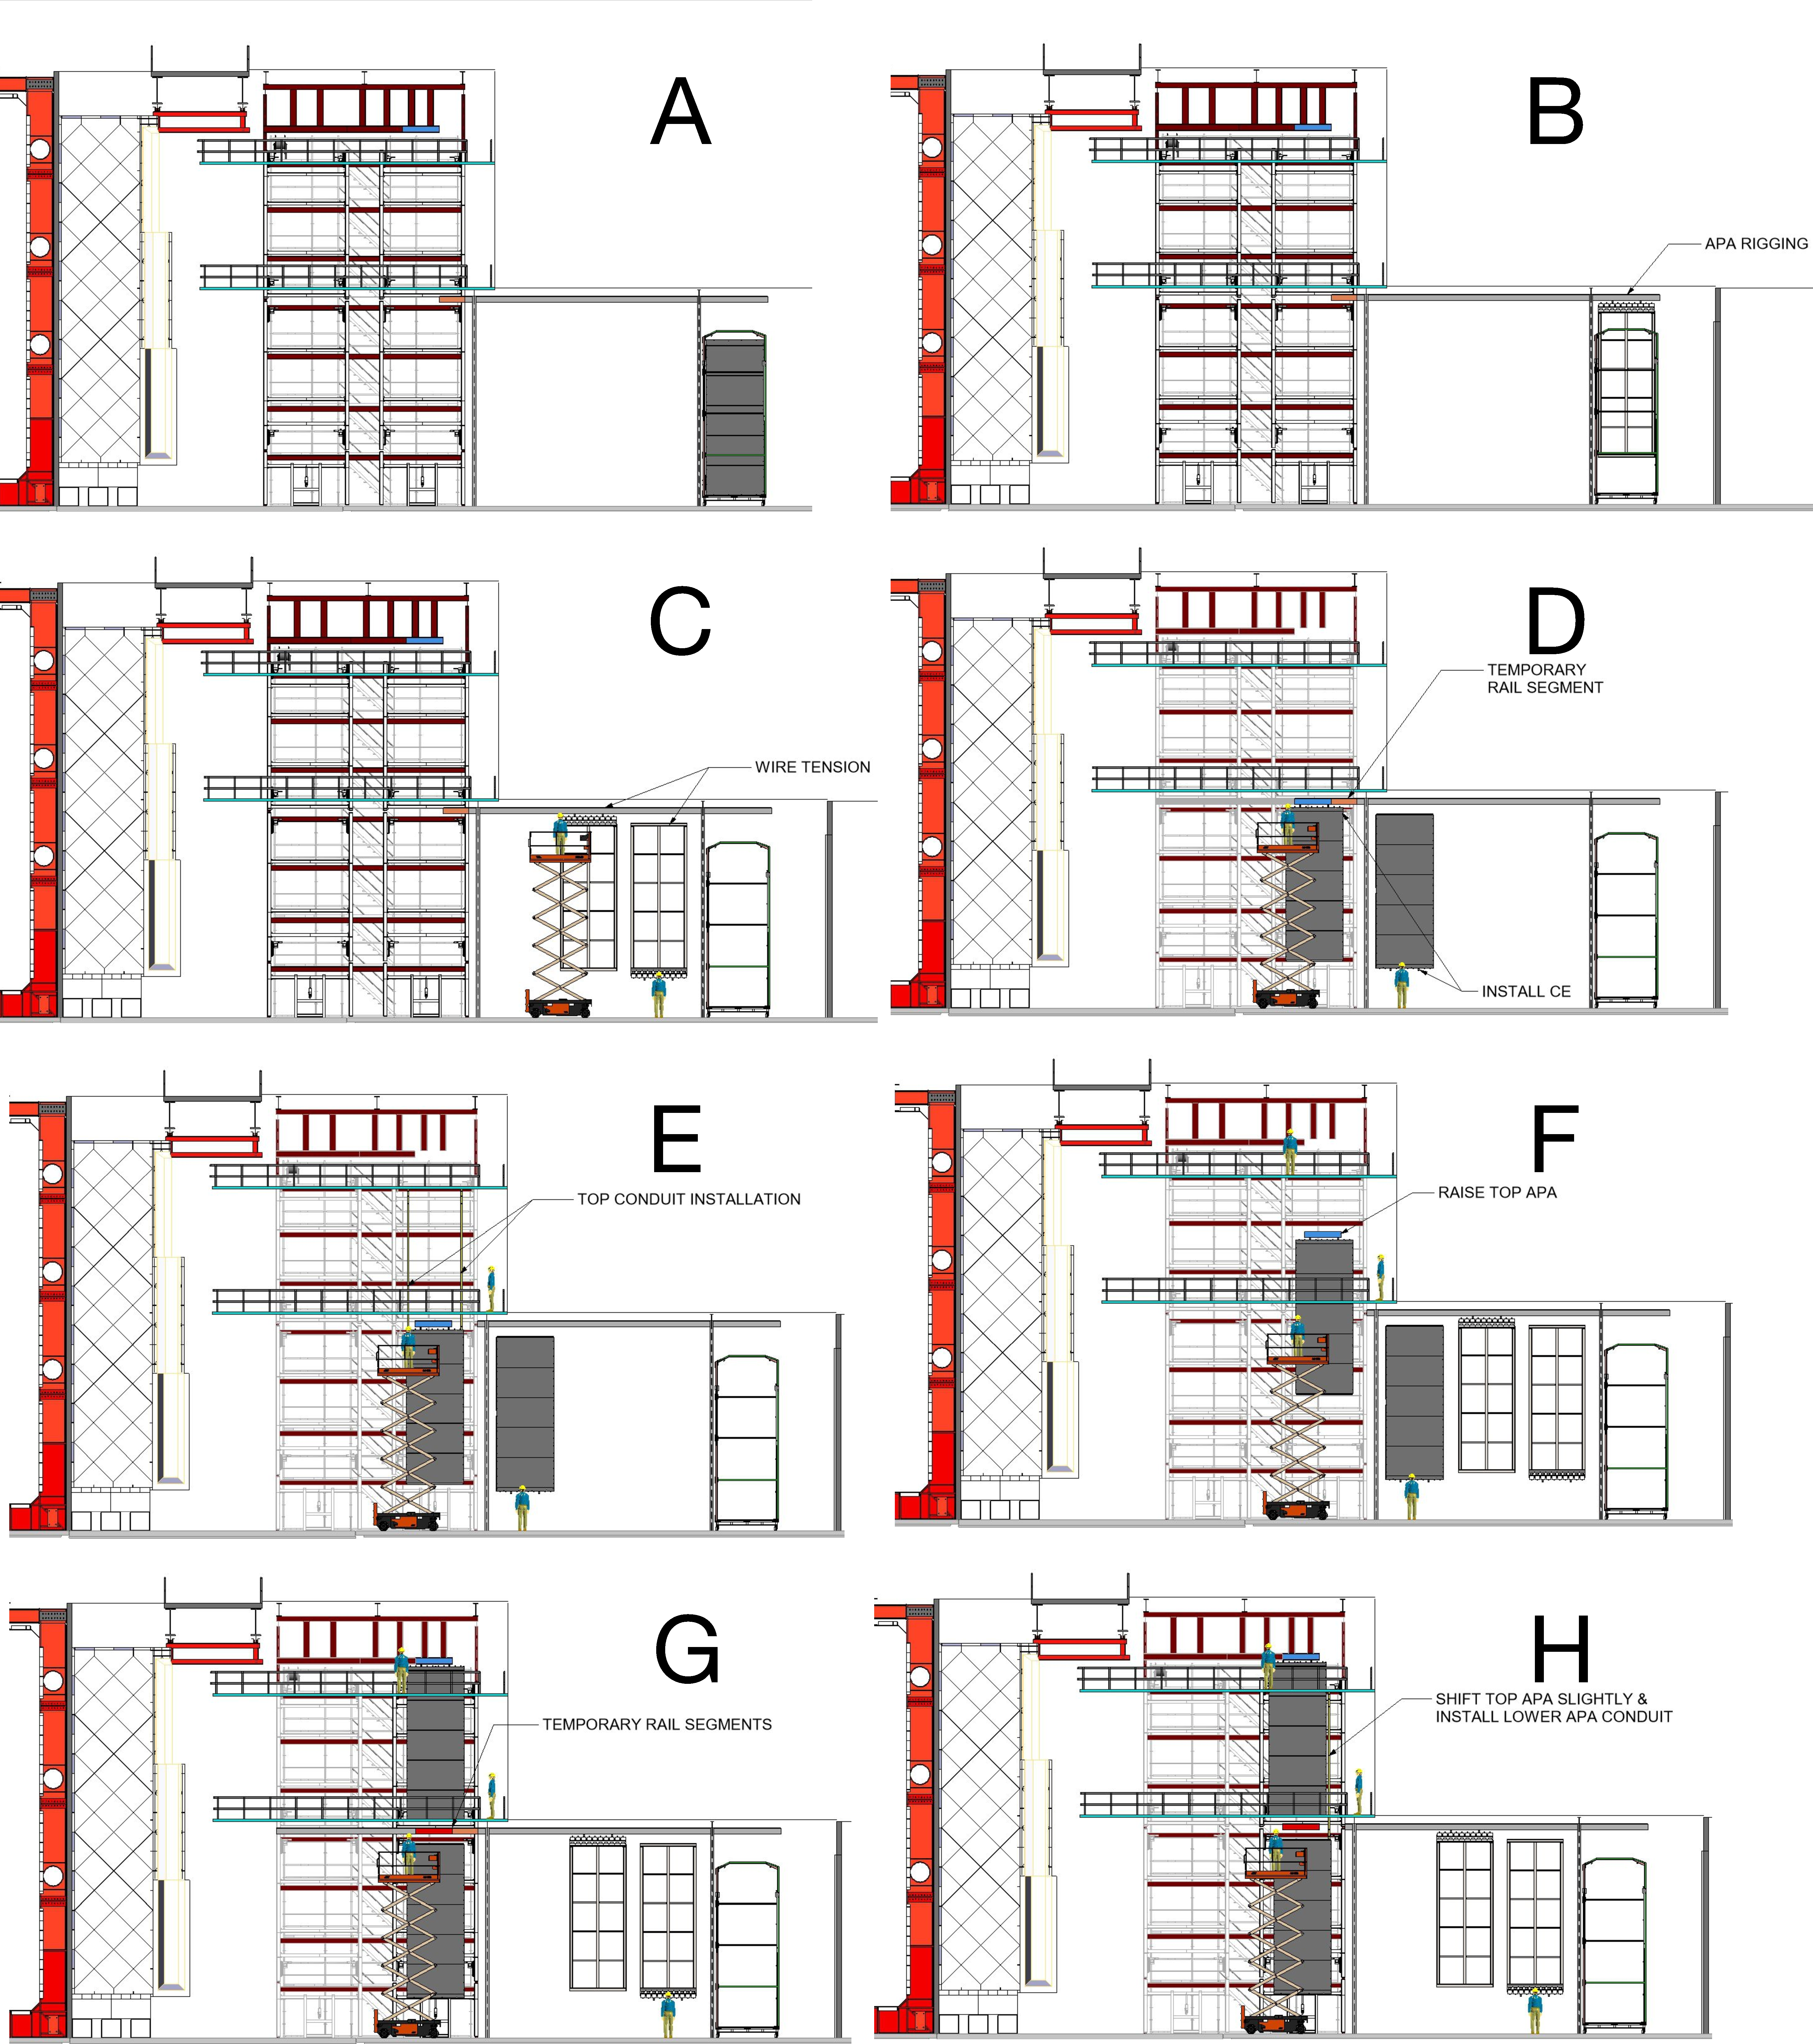
\includegraphics[width=0.95\textwidth]{install-apa-prep}
\end{dunefigure}


First a top \dword{apa} is removed from the transport box and mounted to trolleys on the assembly line rails (Figure~\ref{fig:install-apa-prep} B). 
The \dword{apa} is shifted over to the top \dword{apa} tension measuring station, the protective covers are removed, and a visual inspection performed. 
The bottom of this \dword{apa} cannot support the load of the lower \dword{apa}, so heavy-duty rods are inserted into the sides of the \dword{apa} and bolted to the side tubes using the bolts designed for the linkage connecting the \dword{apa} pair. 
The lower \dword{apa} can then be hoisted out of the transport box and connected to the rail. 
Either the trolleys can be mounted directly to the rods or  a crossbar can be placed between the support rods to hold them.  
Then the lower \dword{apa} can is shifted to its tension measuring location where it is locked in position and its protective covers are removed (Figure~\ref{fig:install-apa-prep} C). 
Wire tension data is collected according to the \dword{qa} plan, similarly to \dword{pdsp}. 
The protective covers are re-installed after the tension measurements to protect the wires during the subsequent assembly steps. 
The top \dword{apa} is moved to the first station on the \dword{apa} assembly tower and attached to a rail section that can be hoisted up to the upper level (Figure~\ref{fig:install-apa-prep} D). 
 
The two short sections of the I-beam rail can be removed to the right and left of the beam segment now supporting the top \dword{apa} and the (\SI{6}{m}) cable conduits installed (Figure~\ref{fig:install-apa-prep} E). 
Once the conduit is in place the I-beam segment supporting the \dword{apa} is attached to a hoist and lifted to the upper rails and attached. 
Locking pins in the \dword{apa} assembly fixture then hold the top \dword{apa} rigidly in position. 
(We will investigate whether the assembly fixture can be modified to allow
the guides to travel with the \dword{apa} when it is lifted, stabilizing it against rotation.)  
The lower \dword{apa} is then moved into position to be connected to the assembly fixtures. 
At this point the  lower \dword{apa} is supported from the bottom, and guides connected to the sides of the \dword{apa} provide mechanical stability while allowing jacks integrated into the lower support to lift the \dword{apa} and the trolleys and rails it was riding on can be removed. 


The conduit is installed by freeing the top \dword{apa} and shifting it slightly to allow its insertion from the top through the foot tube, after which  
the \dword{apa} is moved back into position and again locked to the \dword{apa} assembly fixture (Figure~\ref{fig:install-apa-prep} H).
We then test the lower \dword{apa} \dword{pd} paddles to ensure that everything is working. 
At this point, the upper \dword{apa} is supported by the trolleys that move the \dword{apa}s along the upper transport rails, and it is stabilized using the \dword{apa} assembly frame. There is a \SIrange{300}{500}{mm} gap between the upper and lower \dword{apa}, and the photon cables between upper and lower \dword{apa} can now be connected. 
The connection from the top connectors to the \dwords{sipm} can also be checked. 
To connect the two \dword{apa} modules mechanically, a metal linkage with electrical insulators is inserted into the upper \dword{apa} and bolted into place. Then the lower \dword{apa} is raised until the linkage can be bolted to the lower \dword{apa}.  
The \dword{apa} pair can then be released from the assembly tower supports and jacks; it is now supported from the top, where the upper \dword{apa} connects to the transport rail system. The \dword{ce} boxes can be installed at the top and bottom of the \dword{apa} pair and a simple test of the electronics is performed.  
The \dword{apa}s can now be shifted over to the second station on the assembly tower where the cabling is done.

\begin{dunefigure}[APA cabling and cold test]{fig:apa-assembly-v4}
  { Left: \dword{apa} pair  moving on the cleanroom switchyard and cables being inserted on the tower. Right: the \dword{apa}s being inserted into the \coldbox.
  }
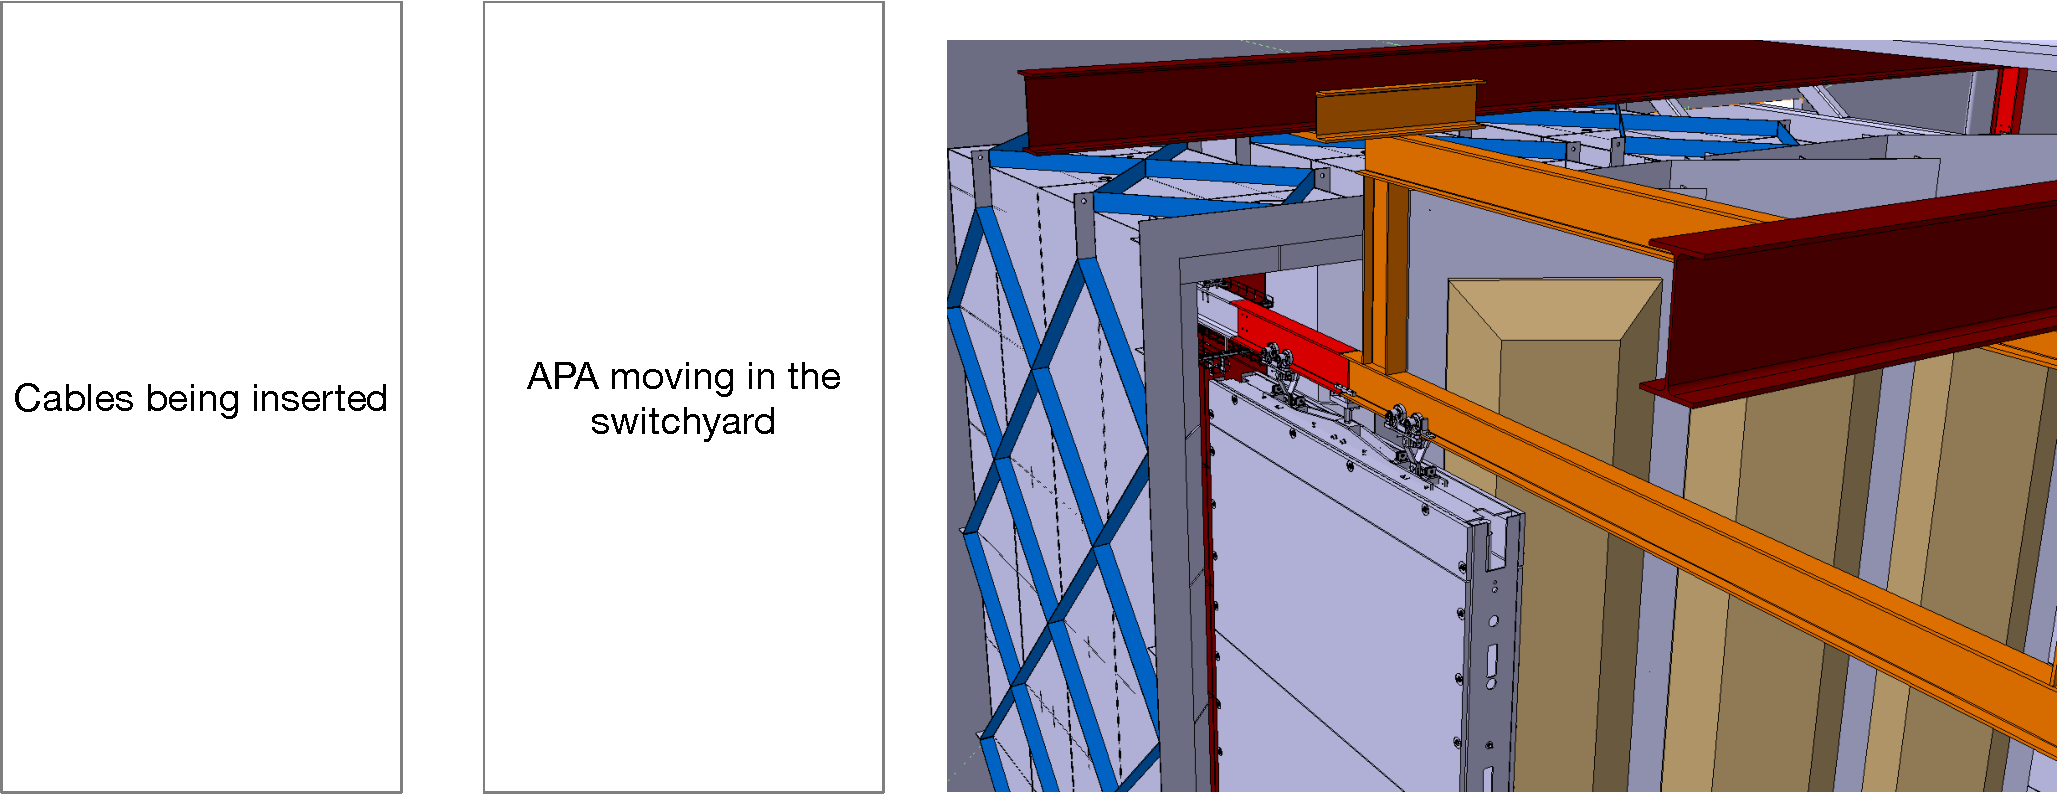
\includegraphics[width=.9\textwidth]{apa-assembly-v4}

\end{dunefigure}

The next assembly step is to install and test the electronics cabling.  The left image in Figure~\ref{fig:apa-assembly-v4} shows the \dword{apa} cabling area on the \dword{apa} assembly tower. 
The electronics cables are delivered to the cleanroom on reels,  pre-bundled and tested. 
The switchyard crane lifts the lower \dword{apa} cable reels to the top of the assembly tower, and a cable is spooled over to a motorized deployment spool. 
The cable guide is then attached and fed through a guide sheave and into the conduit on the side of the \dword{apa}. 
The cable bundle is carefully fed through the conduit and anchored in place using a cryogenic-compatible cable grip. 
The cable is connected to the electronics at the bottom and is laid into the cable trays on top. This process is repeated for the second lower \dword{apa} cable bundle. 
Finally, the upper \dword{ce} and \dword{pd} cables can be installed and prepared for transport.

At this time, the functionality of all the electronics is checked. 
After the \dword{apa} electrical test, the \dword{apa} pair is moved onto the switchyard where the protective covers are removed and the assembly is surveyed using photogrammetry. 
The \dword{apa} pair is then transported to a \coldbox where it undergoes a thermal cycle and complete systems test. 
The right image in Figure~\ref{fig:apa-assembly-v4} shows the \dword{apa} being inserted into the \coldbox. The \coldbox is also a Faraday cage, so noise levels can be measured and the \dword{pds} checked for photon sensitivity. 
After the cold test is complete, an \dword{apa} will either move back to the cabling station (if a repair is needed), or into the cryostat for installation. 


\begin{dunefigure}[CPA assembly steps]{fig:install-cpa-assembly}
  {The \dword{cpa} assembly steps are shown. Top row from left:  \dwords{cpa} are delivered to the \dword{cpa} assembly fixture in the cleanroom; the \SI{3}{m} sub-panels are lifted onto the frame and connected. Bottom row from left: After the \dword{cpa} panel is complete, it is moved into the room and the \dword{fc} modules are attached. The \dword{cpa} is then moved into the cryostat.}
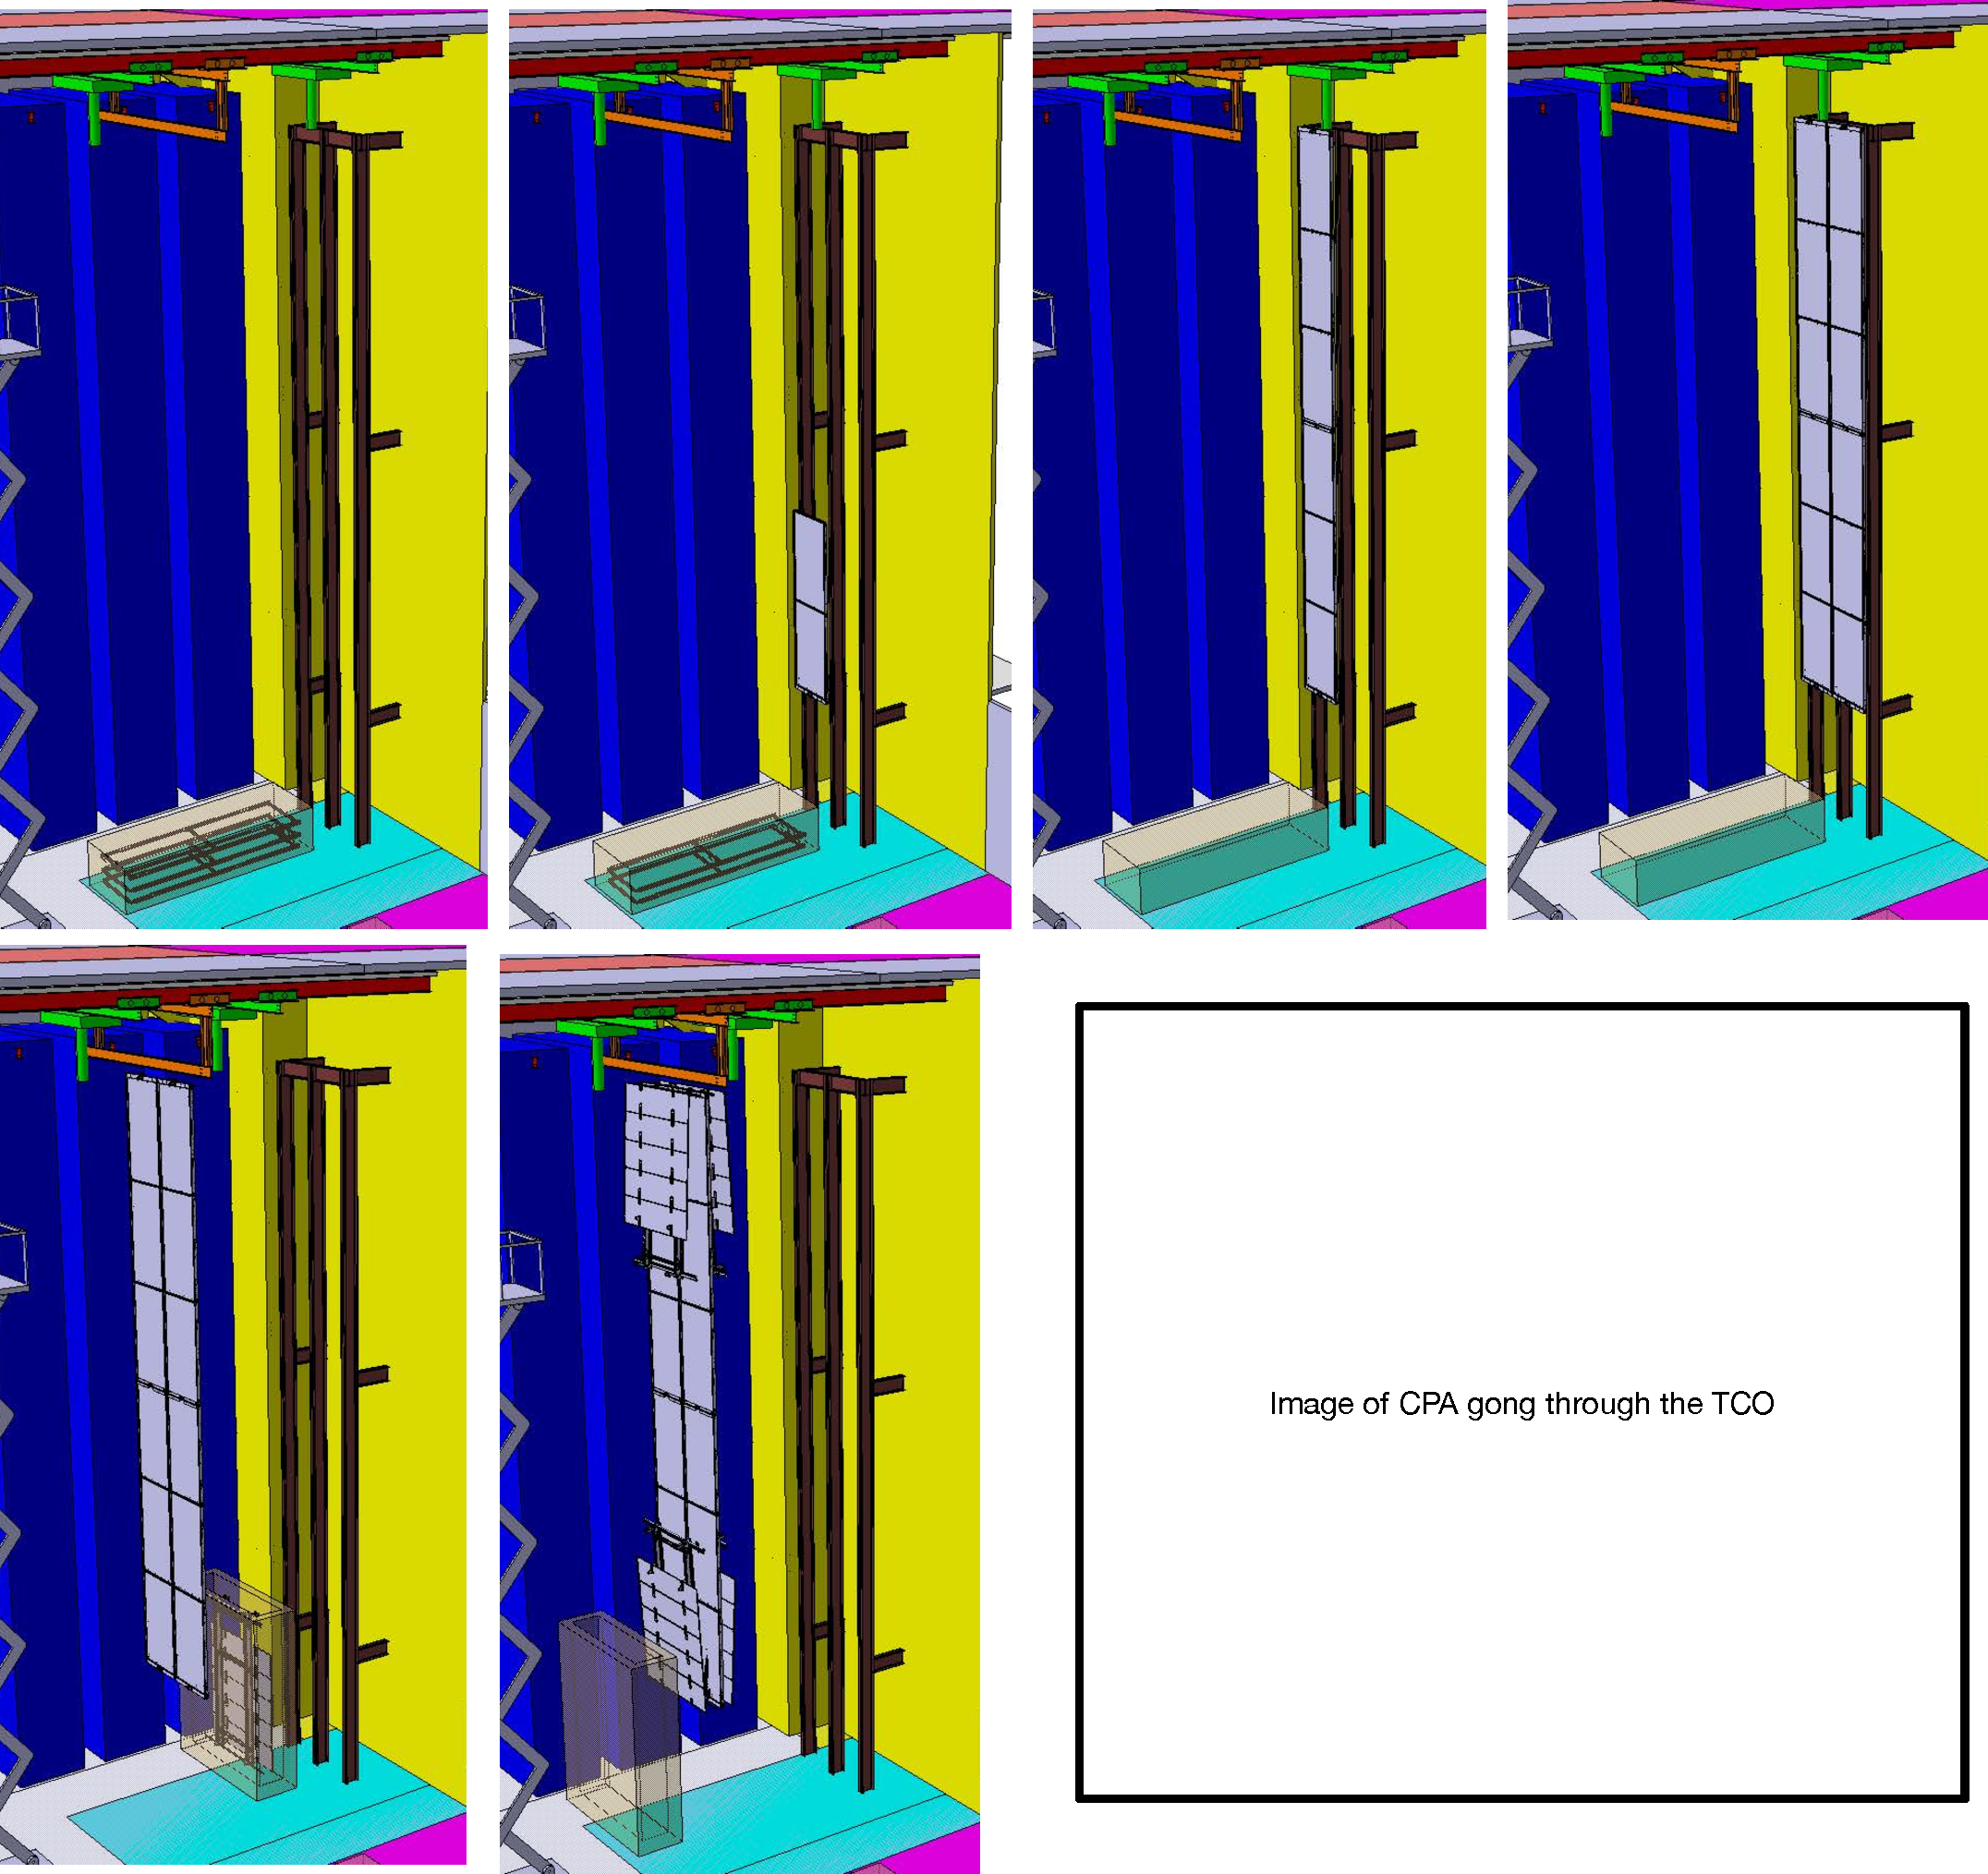
\includegraphics[width=.9\textwidth]{install-cpa-assemble}
\end{dunefigure}

The \dword{cpa} and top \dword{fc} modules are assembled in parallel to the \dword{apa} assembly. Figure~\ref{fig:install-cpa-assembly} shows the  assembly sequence. The \dword{cpa} units are delivered to the airlock in crates that hold six \SI{4}{m} long \SI{1.15}{m} wide units. After cleaning, the crates are brought into the cleanroom and opened. The \dword{cpa} units inside are bagged to provide additional dust protection. They are lifted out of the crate and placed on the assembly frame using the cleanroom switchyard hoist. 
The first two of the \SI{4}{m} tall units are assembled together vertically, followed by third one.
The \SI{12}{m} tall \dword{cpa} panel is then lifted, connected to the installation switchyard, and moved to the \dword{tco} beam. The second \SI{12}{m} tall panel is then assembled like the first from the three remaining \dword{cpa} units in the crate. 
The two \SI{1.15}{m} wide panels are then connected to make the \SI{2.3}{m} wide cathode plane.  
A complete set of \dword{qc} measurements is taken of all electrical connections between units and panels.  
The cathode plane  is then moved to a location in the switchyard where the diffuser fibers and top \dword{fc} modules are then attached. 
Finally, the \dword{cpa}-\dword{fc} assembly is moved into the cryostat.
In Figure~\ref{fig:install-cpa-assembly}, the completed assembly is shown outside the cryostat with the lower \dword{fc} modules also attached. 
This is an option, but present planning is to install the lower \dword{fc} modules once it is inside the cryostat. 


\dword{pd} monitoring system optical diffusers and short optical fibers must be connected to the \dword{cpa} panels before the panels are installed in the cryostat.  
Discussions are underway about the optimal site for this installation:  at the \dword{cpa} assembly facility before shipping to the site, or as part of the assembly of \dword{cpa} stacks in the underground cleanroom.  
Whichever solution is adopted, quartz optical fibers must be routed from the diffuser to the top of the \dword{cpa} assembly to be connected later to the pre-installed fibers in the cryostat; this connection will occur upon final positioning of the \dword{cpa}.  

Work inside the cryostat proceeds in parallel with the work in the cleanroom. 
The large detector components like \dword{apa} pairs and \dword{cpa} modules enter the cryostat using the \dword{tco} rails that connect to the \dword{dss} switchyard. 
Inside the cryostat, the modules are pushed onto one of the switchyard shuttle beams shown in  Figure~\ref{fig:shuttle}. 
The \dword{dss} shuttle beam is then moved to the appropriate row of the \dword{dss}, and  the module is pushed down the length of the cryostat into position. The position of the \dword{dss} beams are well defined and accurately surveyed so that the \dword{apa} and \dword{cpa} modules can be accurately located by precisely positioning them along the \dword{dss} beams. 
A small correction in the height of the modules may be needed to accommodate deflections in the \dword{dss} due to load. Figure~\ref{fig:install-ce-cables} shows the typical situation during the \dword{apa} installation and \dword{ce} cabling. 

\begin{dunefigure}[Cold Electronics cabling inside the cryostat]{fig:install-ce-cables}
  {The installation of the \dword{apa}  and cabling of the cold electronics.
  The left panel shows the \dword{apa}  installation process. 
  One row of \dword{apa}  and \dword{hv} equipment is installed, and a second \dword{apa}  is ready for electrical cabling. 
  The top right image shows the cable trays that will hold the \dword{ce}  cables; one worker is in the scissor lift. 
  The left bottom image shows the work space with the geometry of the \dword{apa}, the cryostat roof, and the cable \fdth .
  }
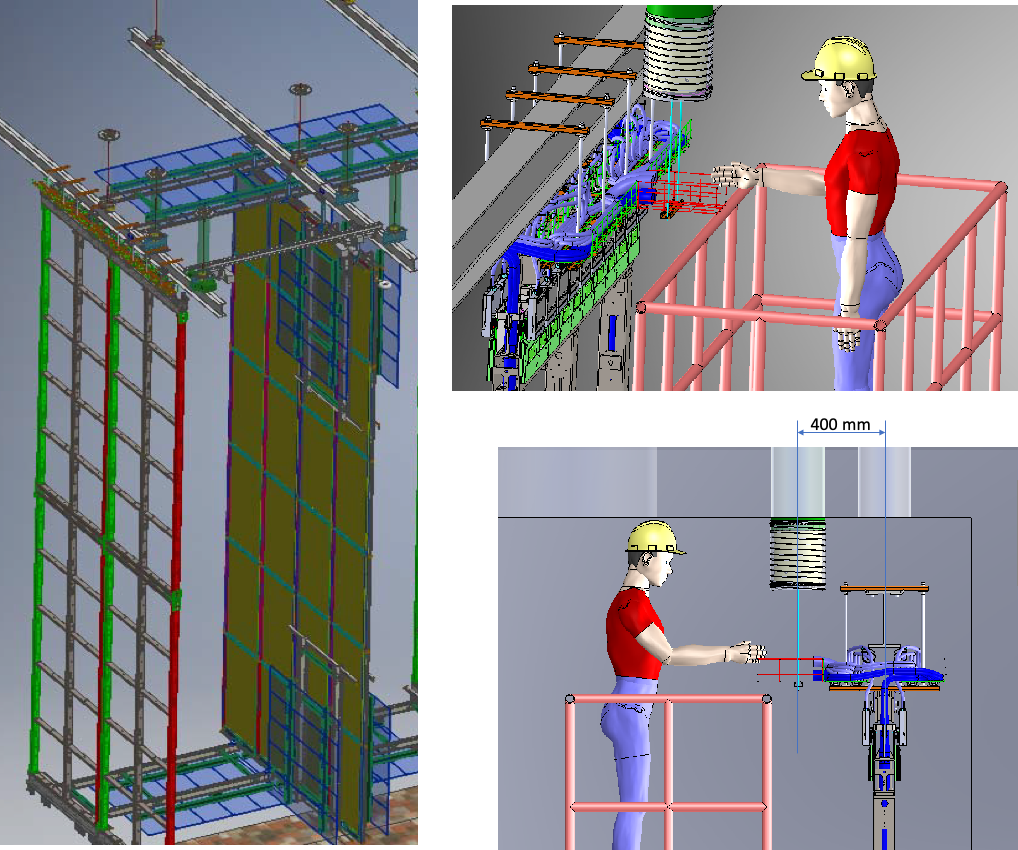
\includegraphics[width=.95\textwidth]{graphics/install-ce-cables.png}

\end{dunefigure}

After the \dword{apa} is moved into position, the permanent support rod is connected to the \dword{dss} beam, and the trolleys are removed. 
The crawler used to push the \dword{apa} along the rails is then moved back through the shuttle area and can be used for the next module. 
After the \dword{apa} is locked into position, the cable tray \fdth to the \dword{ce} is installed, after which \dword{ce} cabling can start. 
Even when a \dword{cpa} module is in position, more than \SI{3}{m} of space remains free between the \dword{apa} and \dword{cpa}, and a scissor lift can easily be positioned in front of the \dword{apa}. 
The two right images in Figure~\ref{fig:install-ce-cables} show the situation at the top of the cryostat during cabling. The cables are not shown, so the cable trays and their support infrastructure can be seen. 

When cabling begins, all the cables are in the cable trays. 
Two people are in the scissor lift in front of the \dword{apa}, and another two people are on top of the cryostat. 
The \dword{ce} cables from the bottom \dword{apa} emerge from the \dword{apa} side-tube  and are split into two bundles in the cable tray for a total of four cable bundles. 
The top \dword{apa} also has \dword{ce} cables organized into four bundles. 
The photon cables from both the top and bottom \dword{apa}s are bundled into two cable bundles.
During the cabling process, each bundle is partly removed from the cable tray and  fed up through the cryostat crossing tube. 
At the top and bottom of the crossing tube  the cables are strain relieved.
This is repeated for each of the ten cable bundles needed for the \dword{apa} pair. 
When all cables are installed through the cryostat crossing tube, any excess length is returned to the cable tray at the top of the \dword{apa}. 
On the roof, the short individual cables are connected to the \fdth  flange, and all electronics and electrical connections are checked. 
At this point the flange connecting the \dword{wiec} can be sealed to the cryostat \fdth flange, and the cable installation is complete. 

Similarly, the \dword{pd} warm cables are connected to the readout module, and the flange sealed after testing.  
Once testing is complete, the support for the tray holding the excess cabling is transferred to the \dword{dss} beam.  
This minimizes any uneven load on the \dword{apa} pair, so they hang more vertically.   
The electronics for each \dword{apa} is continuously monitored after installation. 

Placement and routing of the cables is complex. 
Figure~\ref{fig:install-cable-routing} shows the working \threed model of the cable routing, showing how the cables will be bundled and placed in the trays. 
A mock up the cabling configuration is planned at \dword{bnl}, and the installation of the cables will be tested as part of the Ash River testing program.

\begin{dunefigure}[Model of the electronics and photon detector cabling]{fig:install-cable-routing}
  {Working model of the cable trays and routing of the \dword{pd} cables in the trays.}
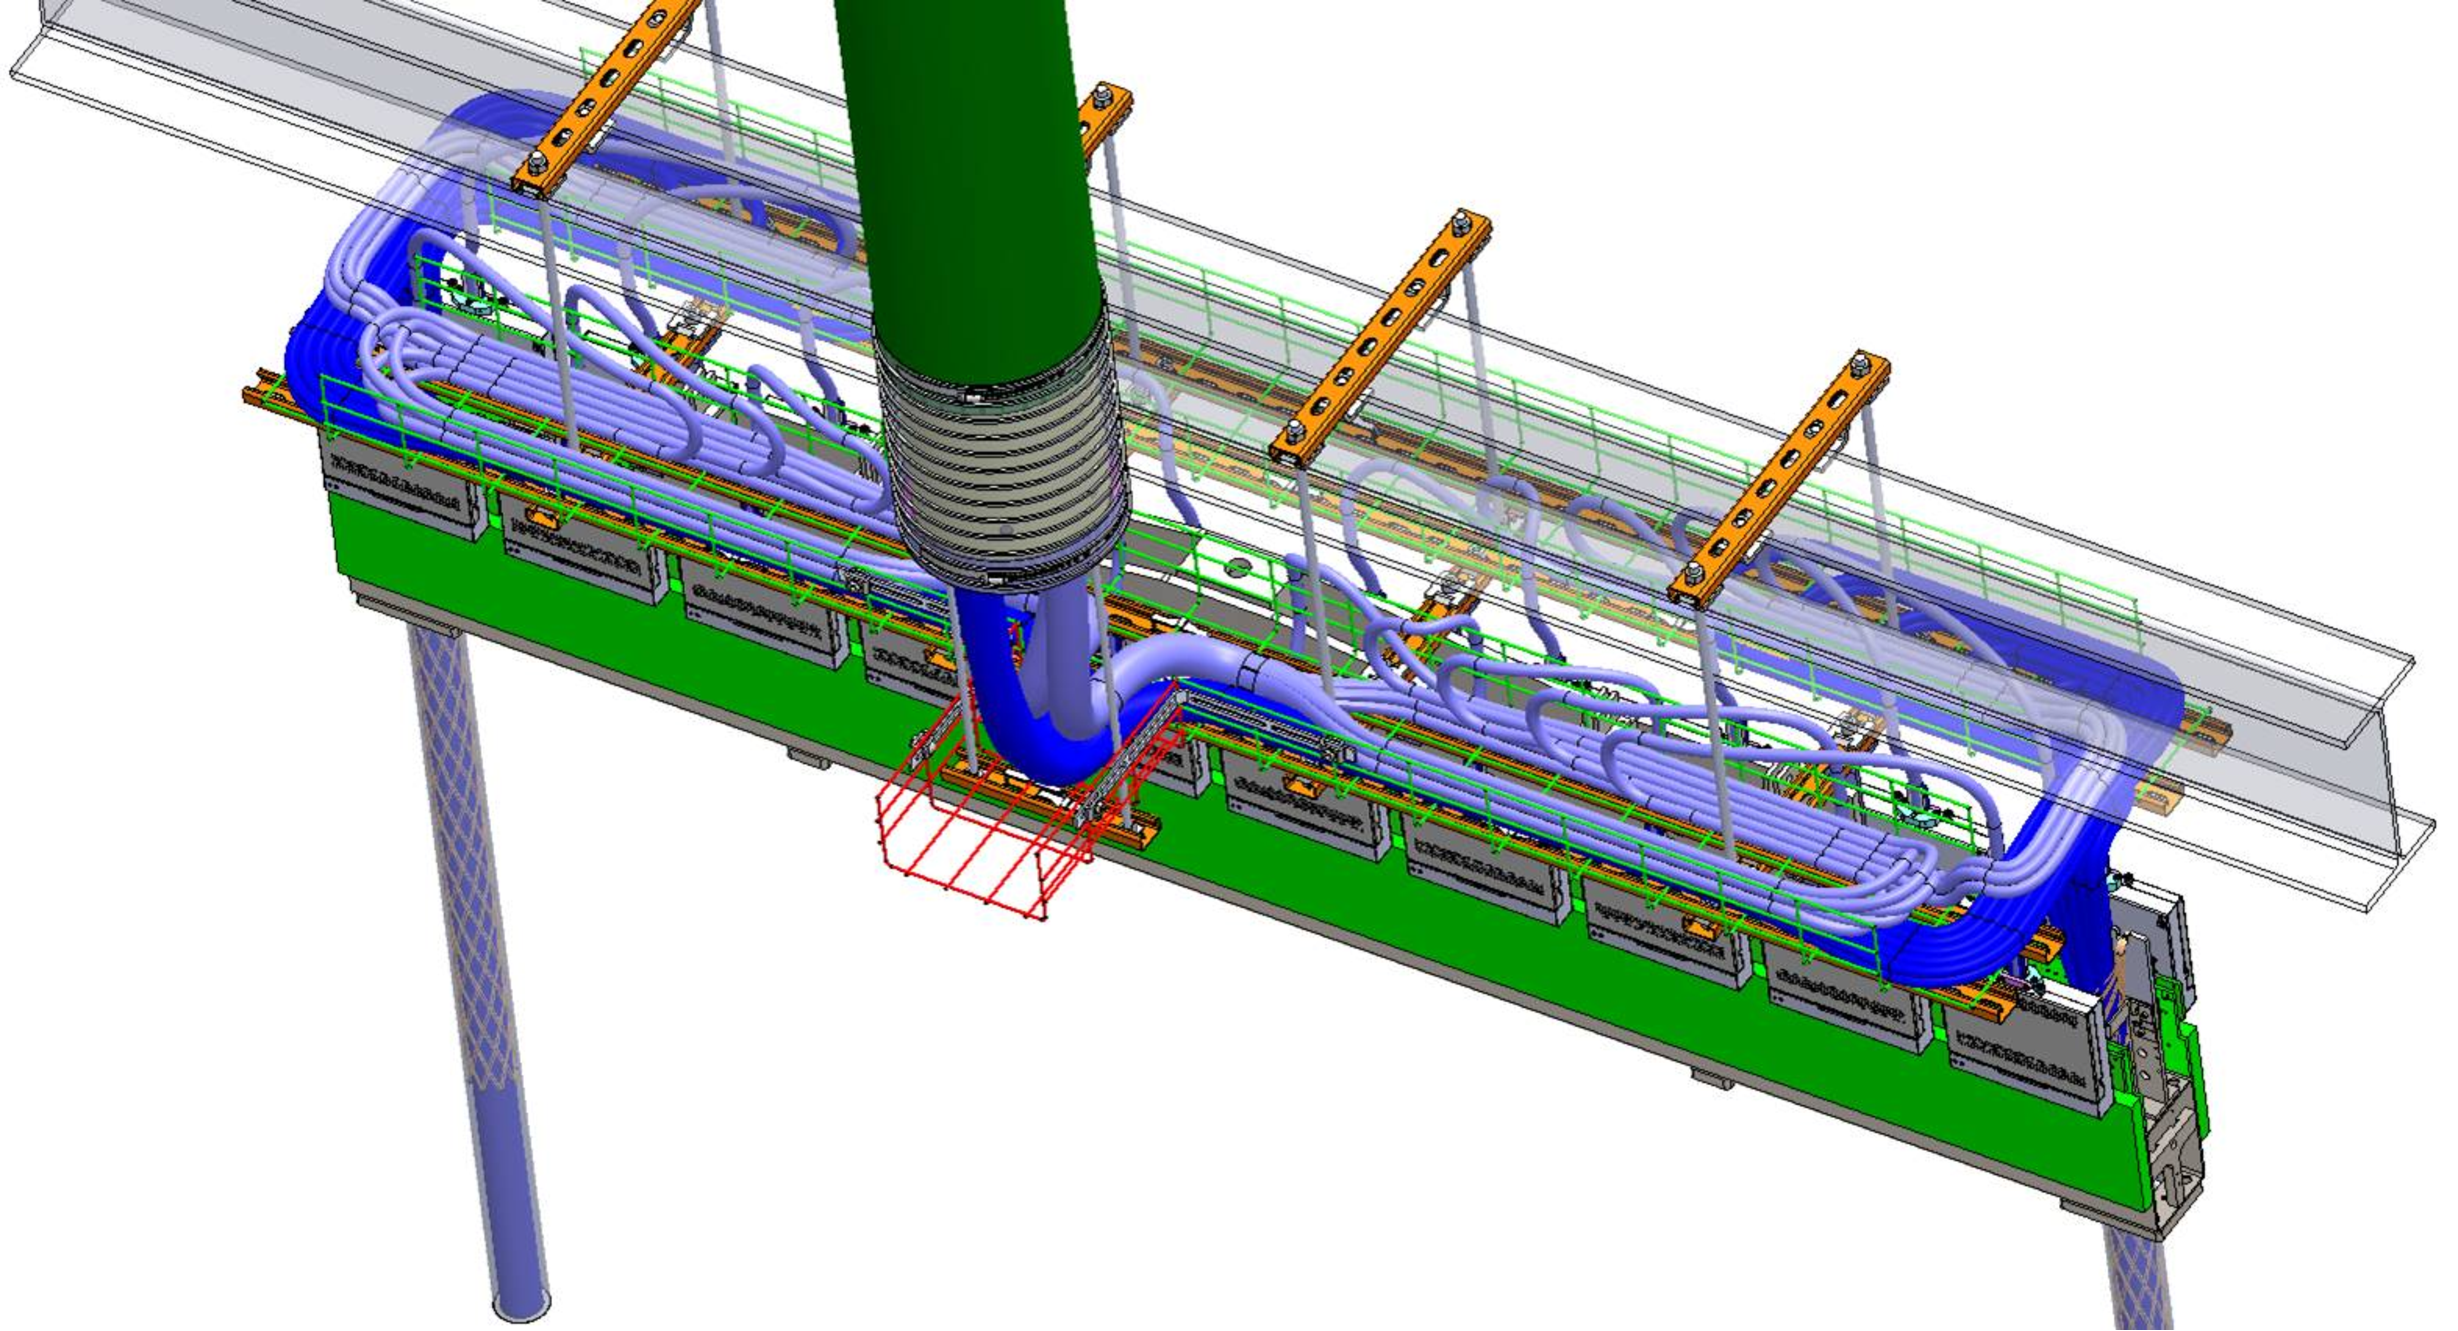
\includegraphics[width=.95\textwidth]{install-cable-routing}
\end{dunefigure}


\begin{dunefigure}[CPA installation]{fig:install-cpa-fieldcage}
  {The top \dword{fc} assemblies are deployed using a custom tool that mounts to the \dword{dss} beams as seen in the top-left panel. The  \dword{fc} is lifted using the electric winch controlled by an operator in the nearby scissor lift. The lower  \dword{fc} is lowered using a hoist mounted on a wheeled frame. The hoist is on a linear slide to keep it aligned above the connection point.}
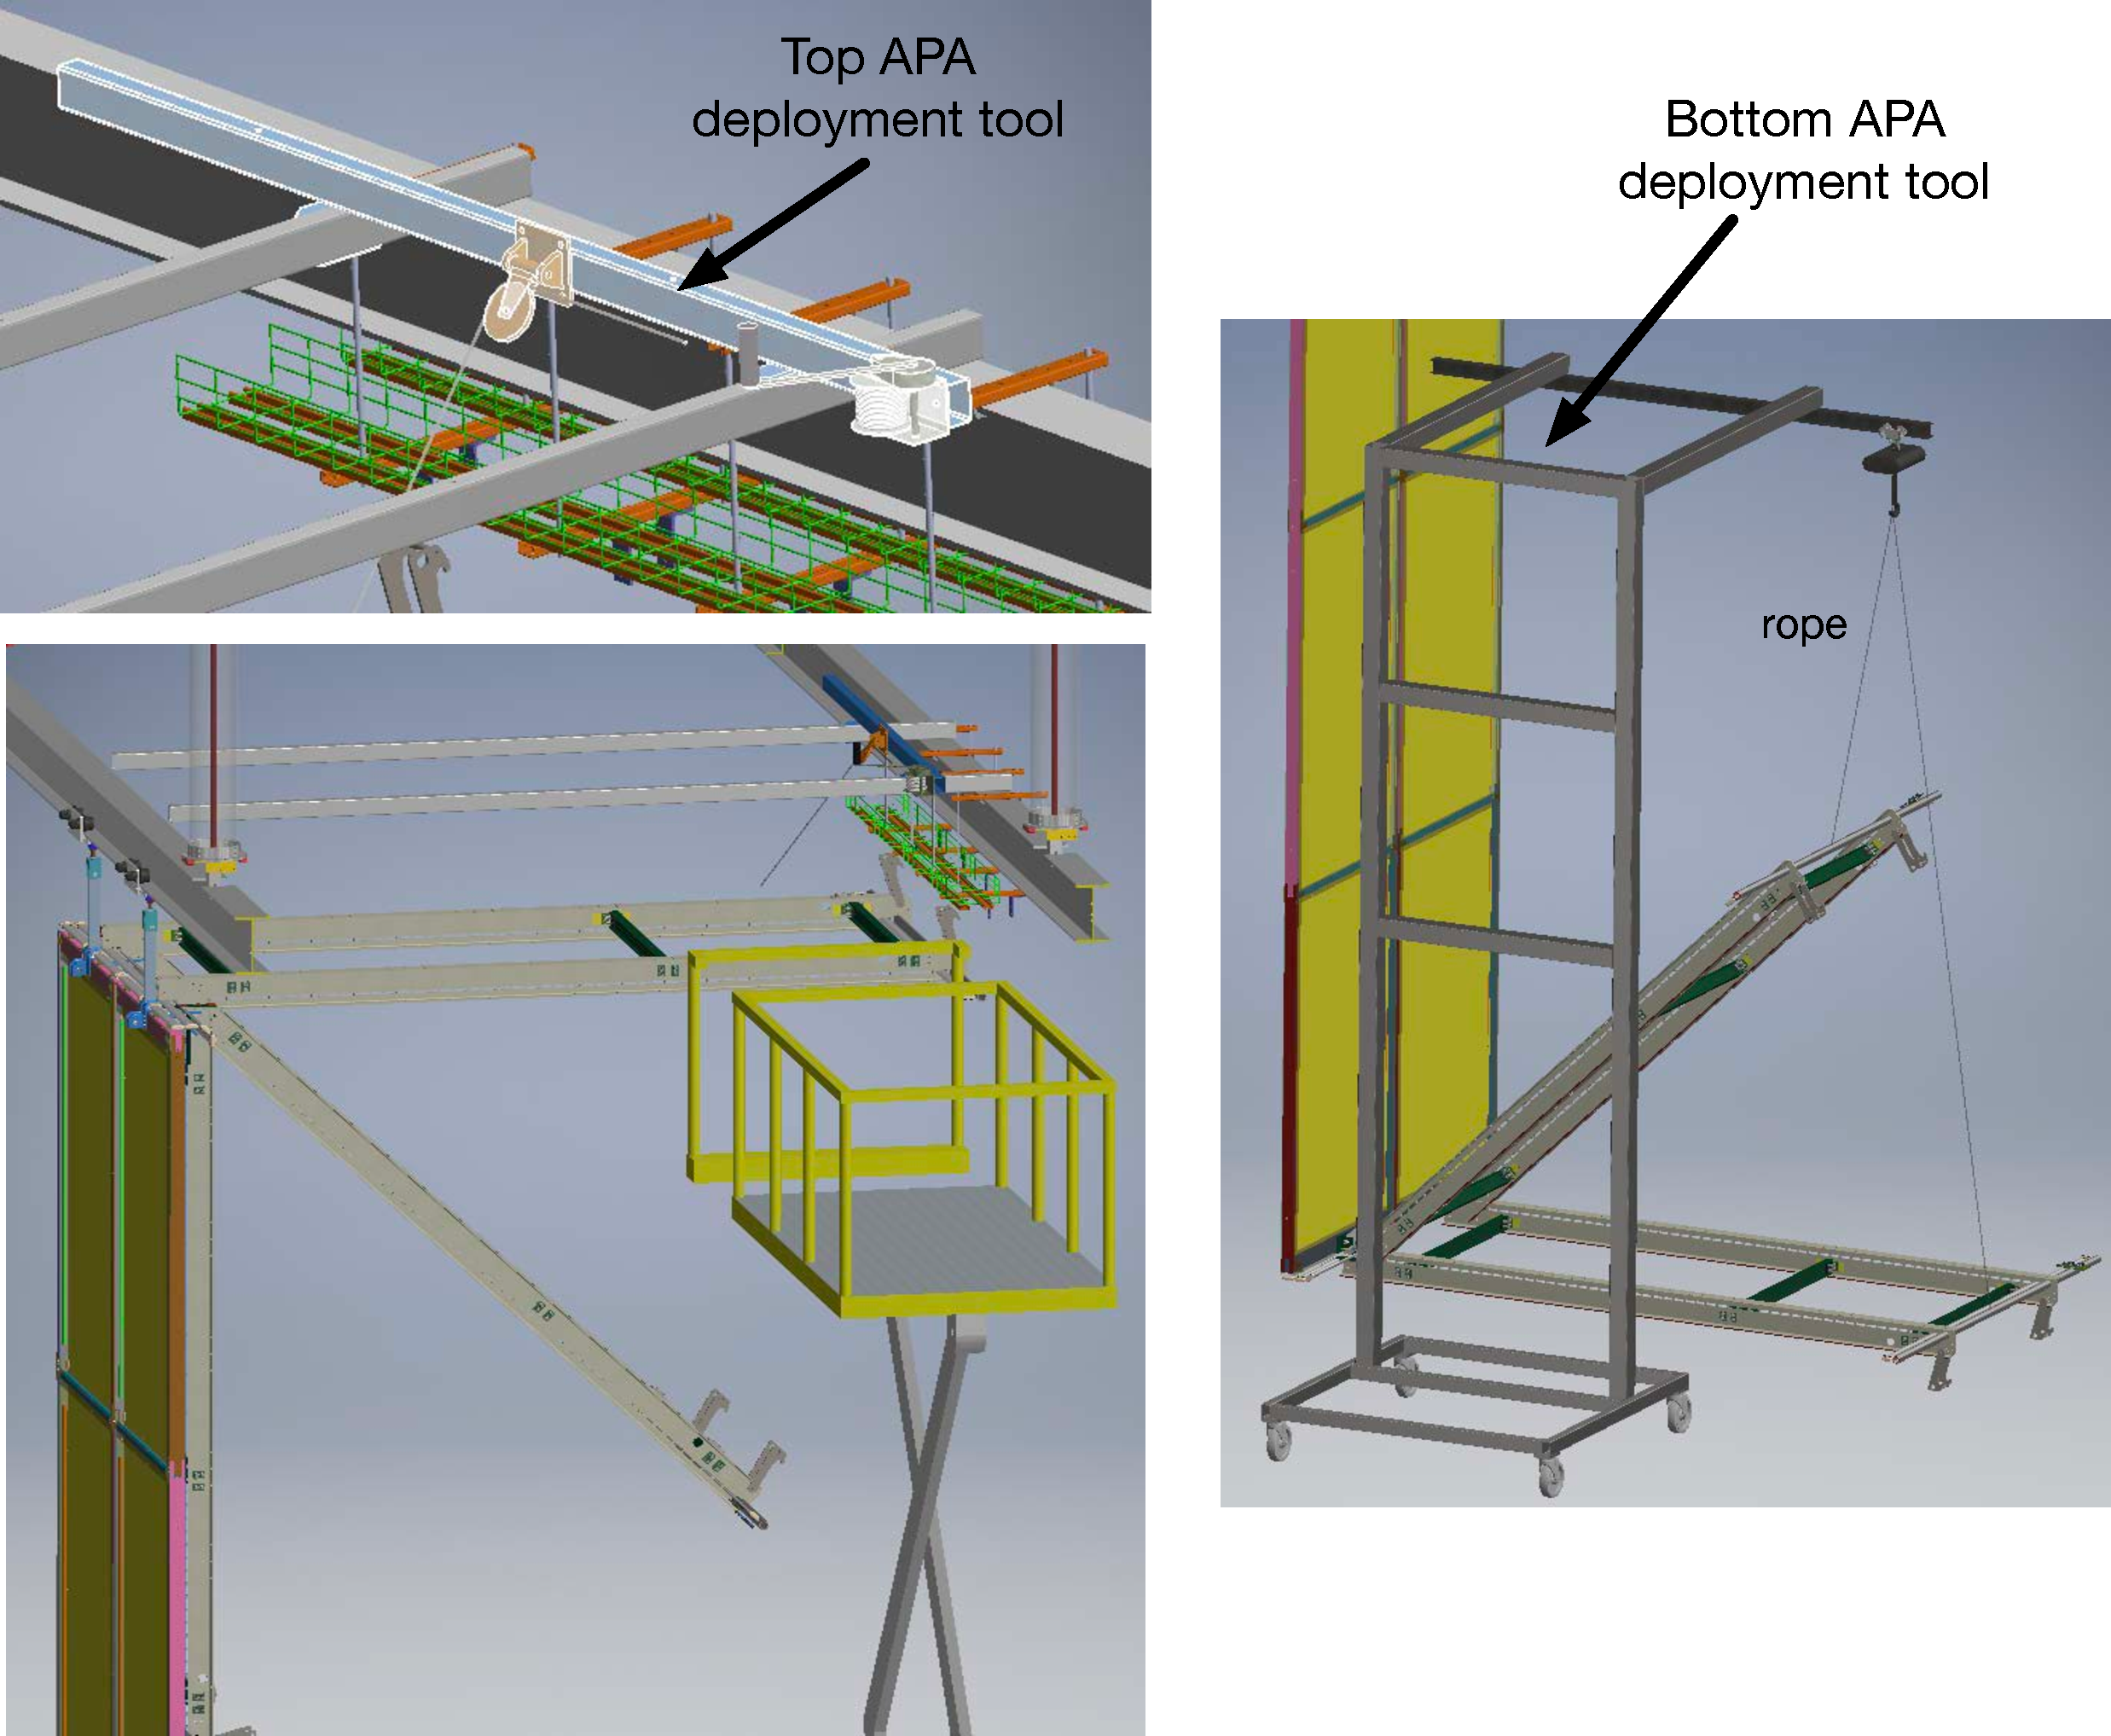
\includegraphics[width=.9\textwidth]{install-cpa-fieldcage}
\end{dunefigure}

The cathode \dword{fc} assemblies are brought into the cryostat like the \dword{apa} pairs, using the overhead rails through the \dword{tco}. 
Inside the cryostat, they are moved into position using the \dword{dss} switchyard and \dword{dss} I-beams. 
Once in position, the load is transferred directly to the \dword{dss} beam, and the trolleys are removed. 
The \dword{cpa} will wait in position until its \dword{apa} pairs are fully tested, after which the \dword{fc} modules could be deployed. 
The deployment sequence of the \dword{fc} has not yet been fixed. 
If the \dword{fc} modules are immediately deployed then the \dword{apa} and \dword{fc} can be tested in the final position. 
If we wait to deploy them, the \dword{ce} can undergo a longer burn-in test and the opportunity to clean the cryostat near the end of the installation is available. 
The decision on the best time to deploy the \dword{fc} will be made during final design.

Figure~\ref{fig:install-cpa-fieldcage} shows the equipment for deploying the \dwords{fc}. 
The top \dword{fc} modules are raised by connecting a cable to the module and then using a pulley-winch assembly to lift the module, which latches to the \dword{apa} mounts. 
A scissor lift is used to connect the cable to the module and also to control the winch. 
After the module is in place, the deployment tool is moved to the next \dword{apa} and \dword{cpa} sets. 
The lower \dword{fc} is deployed using a custom frame that can be wheeled into position. 
The cable from a small hoist is then attached to the \dword{fc} module, and the module can be lowered. 
The hoist is on a linear slide, so the cable is always directly over the connection point, 
keeping the \dword{cpa} from swinging due to an induced moment. 
When the module is down, it latches to the \dword{apa} frame much like the upper \dword{fc}. 
The electrical connections to the \dword{hv} bus are tested, and deployment is complete. 

In principle, the \dword{cpa}-\dword{fc} assemblies can be constructed faster than the \dword{apa}s and %. In theory 
the \dword{cpa}-\dword{fc} assembly process could start later than the start of \dword{apa} assembly if the deployment is postponed. The sequence will be baselined prior to completion of preliminary design.

Periodically during the \dword{tpc} installation the \dword{tco} will be %temporarily 
optically closed and the cryostat made dark to allow testing of the \dwords{pd}. Noise measurements will also be performed during these temporary closures.

The periscopes for the laser calibration system on the top of the \dword{tpc}  can be installed after the nearby \dword{fc} elements are deployed. The lasers are immediately aligned with the alignment laser system. 
Once for each periscope/laser system, prior to the installation of further \dword{tpc} components, the cavern will need to be cleared for the optical alignment as both UV (Class 4) and visible lasers are used.  
This will require special safety precautions, outlined in Volume~\volnumbertc~\voltitletc, Section~\ref{sec:tc-esh-lasers} of this \dword{tdr}.
It may be possible to align all lasers at roughly the same time, to minimize the disruption.

\fixme{Anne -clarify: what is relationship between periscopes and lasers?  The alignment laser system has separate lasers from the laser calib sys? Jim - This is described in the calibration chapter}

\begin{dunefigure}[Installation of final row of detector components]{fig:install-row25}
  {Detector installation as the last row of detector components is installed. At this time, the switchyard runway beams are removed, and the temporary hoists for the \dwords{ewfc} are installed.}
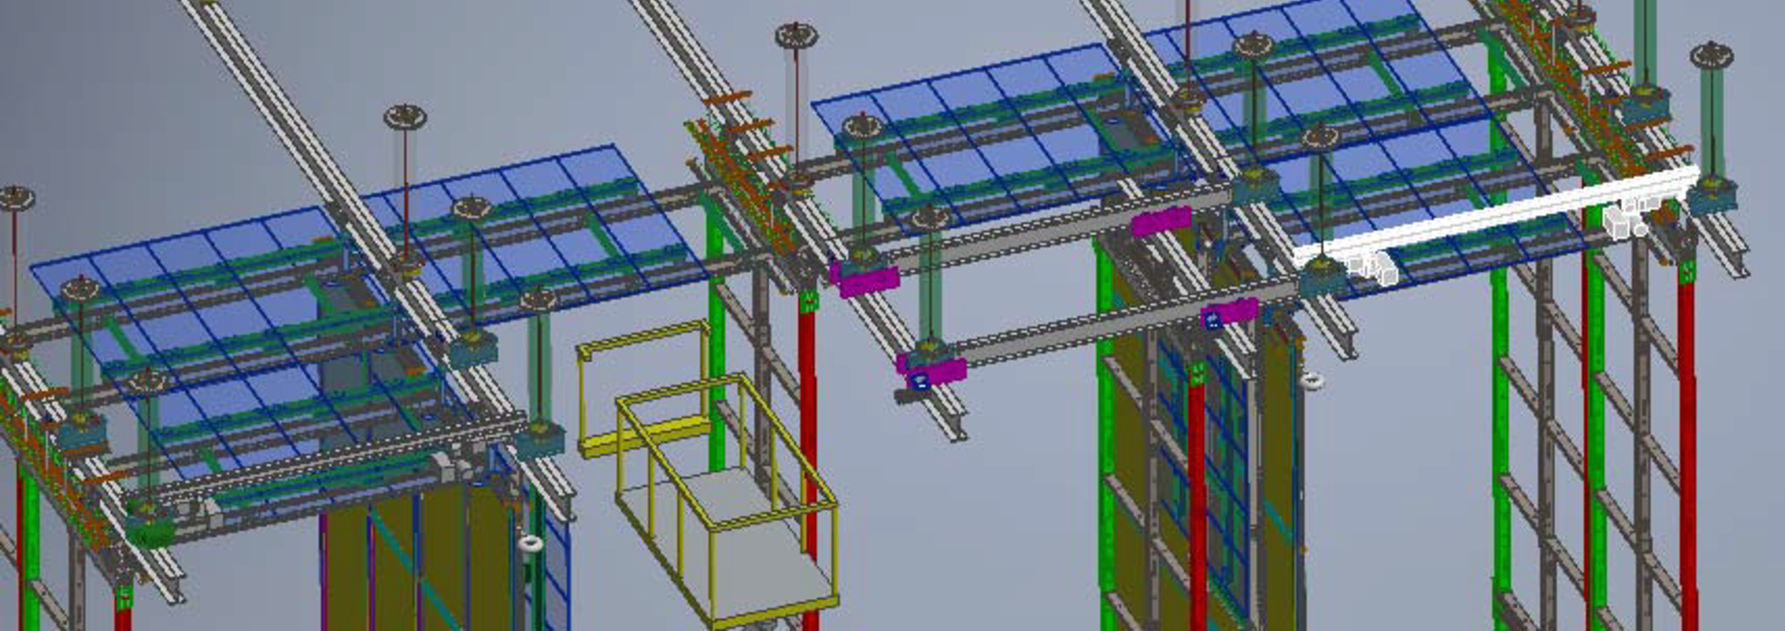
\includegraphics[width=.9\textwidth]{install-row25}
\end{dunefigure}


The last row of detector elements is installed much like previous rows except that the north-south runway beams in the switchyard need to be removed to allow the last row of the detector to contract as it cools down.  Figure~\ref{fig:install-row25} shows the top of the detector as this last row is installed. When the shuttle beam with the detector component is aligned to the correct \dword{apa} or \dword{cpa} row, it is bolted to a short I-beam section of the runway beam which is in turn permanently fixed to the \dword{dss} support \fdth . When the shuttle beams at both ends of a runway beam section are fixed in position, a section of the runway beam is removed and the \dword{ewfc} insertion hoist mounted. The last \dword{fc} modules are then deployed. 

\begin{comment}
%During installation, when a shuttle beam is aligned to a given \dword{apa} or \dword{cpa} row, the short section of the beam is bolted to a short I-beam section of the runway beam that is permanently fixed to the \dword{dss} support feedthrough. When the shuttle beams at both ends of a runway beam section are fixed in position, a section of the runway beam is removed. At this point the last \dword{fc} modules are deployed. The last row of detector elements is installed much like previous rows, but the runway beams of the \dword{dss} switchyard are removed as this \dword{apa} and \dword{cpa} are placed in position. Figure~\ref{fig:install-row25} shows the top of the detector as this last row is installed. \fixme{I need to understand this better. I'm mixing up beams. anne}
This is really confusing. I updated the figures and text
\end{comment}


\begin{dunefigure}[Second endwall FC installation]{fig:install-ew2}
  {Installation of the final \dword{ewfc} before closing the \dword{tco}}
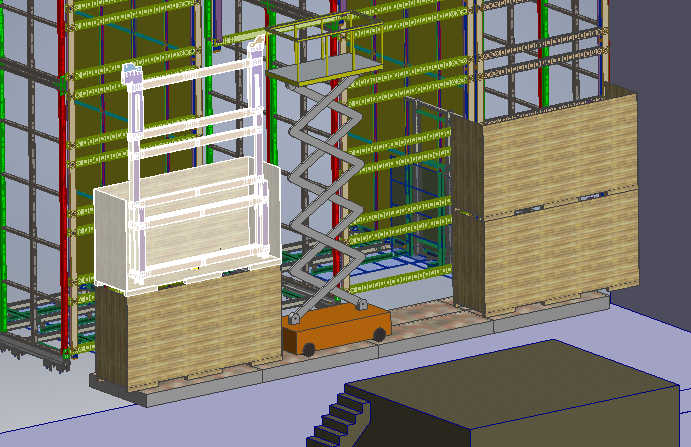
\includegraphics[width=.9\textwidth]{graphics/install-ew2.png}
\end{dunefigure}

The outer two west \dwords{ewfc} are installed like the first one. At this point, the center \dword{apa} is rolled into the cryostat, the shuttle beam is bolted to the \dword{dss}, and the runway beams are removed. The two center drift volumes \dwords{fc} are deployed. The last two \dwords{ewfc} are constructed, and the \dword{tpc} is effectively finished. 

At this point, a frame supported by the shuttle beams is covered with flame-retardant plastic and installed to create a cleanroom work area for the \dword{tco}.  A scaffold is set up for egress to the access holes.
The cryostat will become a confined space area, so the scaffold  must be in place before the \dword{tco} is closed.  Closing the top 3/4 of the \dword{tco} is completed using the \SI{14}{m} scissor lift. The temporary cleanroom area is then removed and the area cleaned. A smaller clean area is constructed to cover the bottom \SI{3.4}{m}  \dword{tco} section. A second scaffold is set up in this space at the end of the cryostat for cleaning and installation of equipment for the calibration and \dword{cisc} equipment.  The scissor lift must be removed at this point. Finally the last section of the \dword{tco} is installed. 


The dynamic T-gradient monitor is installed after the \dword{tco} is closed. 
The monitor comes in several segments with pre-attached sensors and cabling already in place. Each segment is fed into the crossing tube flange one at a time until the entire sensor carrier rod is in place. 
The remainder of the system (the motor system that moves the sensor rod and the sensors) that goes on top of the flange is installed using the bridge crane. 

The purity monitor system will be built in modules, so it can be assembled outside the cryostat leaving only a few steps to complete inside the cryostat. 
The assembly itself comes into the cryostat with the three individual purity monitors mounted to support tubes that are then mounted to the brackets inside the cryostat. The brackets get attached to the appropriate elements (cables trays, \dword{dss}, and bolts in the cryostat corner are under consideration). Also at this time, the remaining level monitors are installed.

The periscopes at the end of the detector are installed and aligned. 

Once all this work is completed, the scaffolding is taken apart and hoisted out the access holes along with all remaining flooring sections. The area is cleaned, and the last two workers in the cryostat are hoisted out. 

The warm inspection cameras and other possible calibration instruments can be installed from the roof while the \dword{tco} is being closed. 
After the \dword{tco} is closed the four access holes (2 ventilation and 2 personnel access)  can be closed and the pulsed neutron source can be placed in position above two of the access holes. The pulsed neutron source can be tested to confirm neutron yields with integrated monitors and dosimeters in dedicated runs.

% clear the figure buffer before starting the next section
%\clearpage




%%%%%%%%%%%%%%%%%%%%%%%%%%%%
\subsection{Installation Prototyping and Testing (QA/QC)}
\label{sec:fdsp-tc-inst-qaqc}

The section first below describes the planned \dword{qa} process for developing the installation process and qualifying the installation equipment; the \dword{qc} testing planned during the detector installation follows. 

\subsubsection{Detector Installation Quality Assurance}

An extensive prototyping program designed to develop and test the \dword{pdsp} installation process was executed in the \dword{nova} Assembly Area at Ash River prior to the final design of the \dword{protodune} detector. 
The \dword{nova} Far Detector Laboratory at Ash River is owned and operated by the University of Minnesota using grants from the \dword{doe} and \dword{fnal}.
A mechanical mock-up of one sixth of the detector was fabricated from test components where the interface infrastructure was considered final. 
Here all the mounting points, external dimensions, loads, latches and hinges were expected to be exactly as planned for the final \dword{pdsp} detector.
A mock-up cryostat roof and wall were constructed to understand how some tasks could  be performed physically in the space available.
Initially, all the components failed the installation test and had to be modified. A series of hands-on working group meetings with the different consortia were held to resolve installation issues and revise the detector design. 
In some cases two iterations were required before the components could be assembled together in the space available and dedicated tooling had to be developed. 
Having the mock-up of the cryostat roof and walls was critical in developing the installation procedures and eventually assembling \dword{pdsp} on schedule; only in handling these objects in the space available were all the constraints obvious. 
The experience gained during the \dword{protodune} Ash River trial assembly was critical for both verifying the mechanical design and interface, and also for developing the tools and procedures needed for the installation.

The \dword{dune} \dword{tpc} will have half the available work space,  both above and below the \dword{tpc} inside the cryostat, compared to \dword{pdsp}. 
We learned from \dword{pdsp} that access at the top and bottom of the detector was already 
difficult and properly connecting the bottom latches between the \dword{fc} and the \dword{apa} during the \dword{fc} deployment was challenging. 


The process of test installing the detector mock-up allowed refinement of the hazard analysis and development of the detailed procedure documentation for the assembly process. 
Having complete, well developed procedures prior to the delivery of the components at \dword{cern} allowed the safety approval process to begin early and along with the test installation, created a safe work environment.


Mechanical tests at the \dword{dune} trial assembly at Ash River will be key to developing the installation process. We will also perform the time-and-motion studies that are required to develop a reliable schedule.  Other important prototyping tasks performed at  universities, national laboratories, and \dword{cern} will contribute to the installation plan. 
For example, \dword{anl} is testing the \dword{apa} shuttle beam drive system and the \dword{cpa} assembly tower connections before they are shipped to Ash River, and \dword{bnl} is planning a test setup to develop the cable management process on top of the detector. 
The \dword{pdsp} experience has led to many small improvements in 
in the assembly process, and the \dword{spmod} prototyping effort will help us develop it further. 


\begin{dunefigure}[NOvA Assembly Area at Ash River]
{fig:NOvA-Assembly-Area}
{Top Panel shows the \dword{nova} Assembly Area and the bottom panel shows the \threed model of the installation prototype.}                
%\centering     %trim=left bottom right top, clip
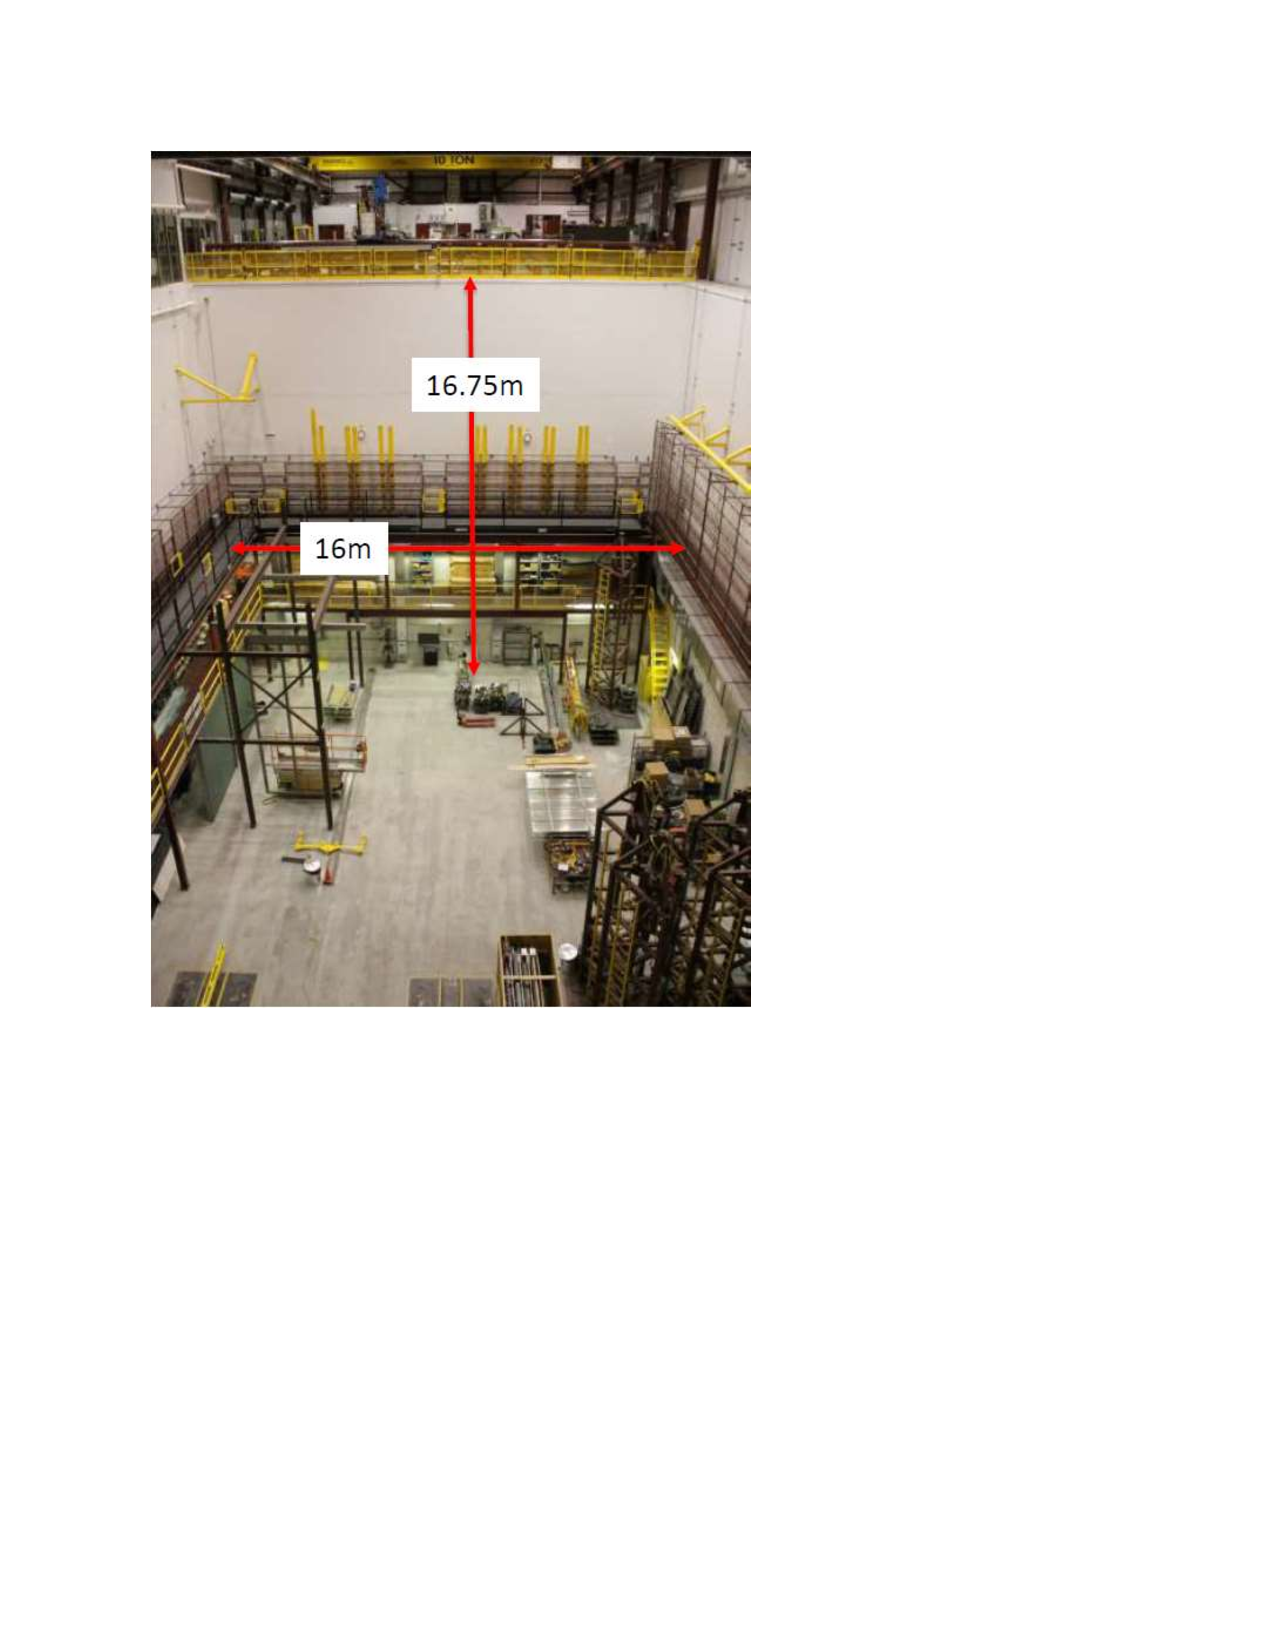
\includegraphics[width=0.49\textwidth]{NOvA-Assembly-Area}
\vspace{-12pt}
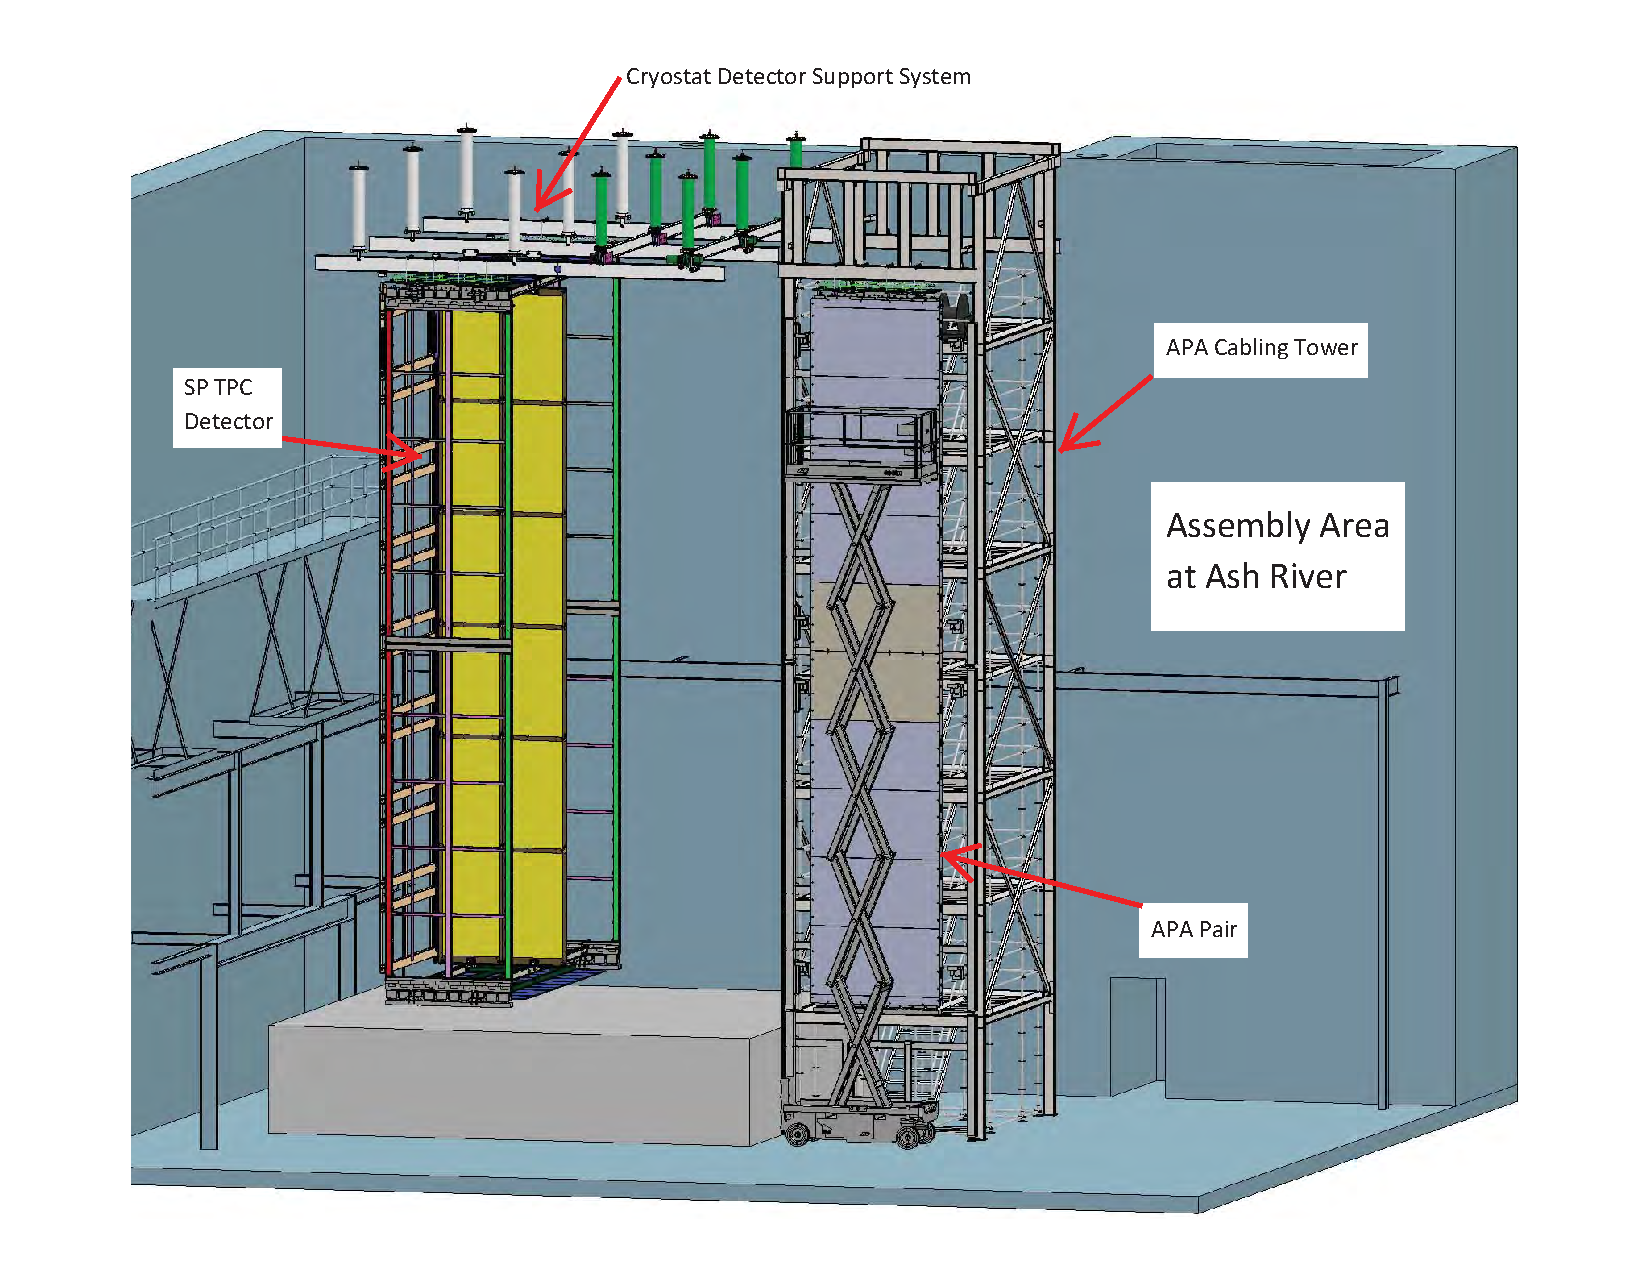
\includegraphics[width=0.7\textwidth,trim=0pt 0pt 0pt 0pt,clip]
{DUNE-Trial-Assembly-Ash-River}
\end{dunefigure}

Full-scale mechanical testing of the assembly and installation of all the \dword{tpc} components, including the \dword{dss}, will be critical for the success of the \dword{spmod}. 
A prototype of the installation equipment for the \dword{spmod}  will be constructed at the \dword{nova} neutrino experiment \dword{fd} site in Ash River, Minnesota, USA, and the installation process tested with full-scale mechanical models detector elements.  
This assembly area at Ash River, shown in Figure~\ref{fig:NOvA-Assembly-Area}, meets the requirements of both space and available equipment, and experienced technicians that helped construct the \dword{pdsp} detector are available. 
It has both the elevation and floor space available to do a full-scale test of both the component assembly outside the cryostat and a test installation of the \dword{tpc} components  inside the
cryostat. 
Also available are a \SI{75}{ft}$\times$\SI{100}{ft} loading dock and ramp access, two \SI{10}{t} cranes, a machine shop, and a wide assortment of tools. 

While the University of Minnesota has jurisdiction over the safety program at \dword{ashriver}, the facility also follows the \dword{fnal} Safety Program and works together with \dword{fnal} to ensure a safe working environment.  
A key deliverable of the \dword{pdsp} work was the set of documentation, including e.g.,   
component design,  hazard analysis, and final assembly procedures, for approval by the \dword{cern} Health Safety and Environment division. 
For Ash River and \dword{dune}, this is all part of the \dword{orc} review process. 
Documentation for both the trial assembly process at Ash River and for \dword{dune} will be stored on the \dword{edms} at \dword{cern}. 
Though many of the \dword{tpc} components are mechanically similar to the \dword{pdsp} components, the access equipment will be different and the need to work at \SI{14}{m} height will make construction of the \dword{spmod} much more challenging.  


The \dword{dune} \dword{fd} trial assembly program at Ash River has the following goals:

\begin{enumerate}
\item Validate the \dword{apa} design. 
\item Test all full-scale \dword{tpc} components during both the initial assembly stages in the cleanroom outside the cryostat and the deployment stages inside the cryostat:  
\begin{itemize}
    \item \dword{apa}  assembly: manipulation of \dword{apa} shipping frames, joining an \dword{apa} pair together, \dword{ce} cabling, removal and re-installation of the \dword{apa} protection covers, movement on shuttle beam, cryostat cabling, and final deployment in cryostat. 
    \item Integration and installation testing of \dword{pd} components: cable harness routing and cryogenic cable strain relief, module integration into \dword{apa} frames, and electrical connections between upper and lower \dword{apa}s.   Mounting of \dword{pd} monitoring system components and optical fiber routing on the \dword{cpa}. %will be tested.
    \item \dword{dss} and shuttle beam system, including final detector configuration.
    \item Assembly of \dword{hv} system: construction of an \dword{ewfc}, %endwall, 
    \dword{cpa} pairs, movement on shuttle beam, and final deployment in cryostat.
\end{itemize}
\item Write full set of hazard analyses and assembly procedure documents; %including gathering 
gather all component documentation. 
\item Test access equipment (scaffold, scissor lifts, work platforms) and lifting fixtures. 
\item Study assembly time and motion, including labor estimates. 
\item Train lead workers as \dword{dune} begins set up (in the installation setup phase).
\item Test mechanical modifications.
\item Train the installation team prior to the start of \dword{dune} installation (in the installation phase). 
\item Possibly (in future) run assembly tests of the \dword{dpmod} components.
\end{enumerate}


%In order to meet the above goals a staged testing program has been developed.  The initial phase is dedicated to qualifying the \dword{apa} and \dword{fc} designs. The main difference (other than the number of units) between \dword{protodune} and  \dword{dune} is that the \dword{dune} detector is twice as tall. This is achieved by hanging one \dword{apa} beneath another. Unfortunately the \dword{apa} built for \dword{protodune} were not designed for this so the cables from the lower \dword{apa} could be routed through the upper \dword{apa} thus requiring a major redesign. To date a pair of \dword{apa} has never been assembled or cabled. The handling of the lower \dword{apa} and the assembly into a double has also never been tested. As shown in \dword{protodune} these tests are critical and must be completed before the design of the \dword{apa} is final. The initial phase of the installaiton testing is focused on this and is time critical as the work must be complete before \dword{apa} production can begin in 2020. In parallel to the \dword{apa} testing the assembly of the \dword{cpa} and the deployment of the \dword{cpa} can also be tested as they will not require large amounts of additional infrastructure.

A staged testing program has been developed to meet the above goals.  The initial phase is dedicated to qualifying the \dword{apa} and \dword{fc} designs. The main difference (other than the number of units) between \dword{pdsp} and the \dword{dune} \dword{spmod} is that one \dword{apa} will hang beneath another, doubling of the height. The cables from the lower \dword{apa} will need to be routed through the upper \dword{apa}, thus requiring a redesign. 

To date, an \dword{apa} pair has never been assembled and cabled. It is critical to complete tests of these operations before finalizing the \dword{apa} design. The initial phase of the installation testing is focused on this; it is time critical, so that \dword{apa} production can begin in 2020. The assembly and deployment of the \dword{cpa}s can  be tested in parallel since they will not require large amounts of additional infrastructure.

The second phase of the prototyping program is focused on developing the installation plan and verifying all the detector interfaces. 
We will construct a full-scale model of the major installation equipment in the cleanroom and the inside of the cryostat and conduct a dry run of the assembly, component transport and deployment in the cryostat. 
This is especially important because the space in the \dword{spmod} cryostat above and below the detector is only half that of \dword{pdsp} where some of the installation steps were already challenging.

The final prototyping stage includes a mock-up of the top of the cryostat to test the final cabling steps at height and perform  accurate time-and-motion studies to benchmark the installation schedule. Detailed procedures will be drafted and in place before the start of actual installation. The installation team will train to work underground at this time.


Testing the installation process early allows identification of  hazards and remediation measures -- without the time pressure associated with the actual installation. This is critical for reducing risks.  Detector installation is by definition on the critical path, making it vital that the work be performed efficiently and with the lowest possible risk. 

This prototyping program is summarized in Table \ref{tab:AR-test-program} and the \threed model representing the final layout is shown in Figure~\ref{fig:NOvA-Assembly-Area}. 

\begin{dunetable}
[Summary of the tests at Ash River]
{p{.2\textwidth}p{.7\textwidth}} %{ll}
{tab:AR-test-program}
{Summary of the tests at Ash River} 
Testing phase & Deliverables\\ \toprowrule
FY-19 20 Phase 0   &  \\ \colhline
 & Build an APA cabling tower for full scale APA pair assembly \\ \colhline
 & Check vertical cabling with a pair of APA side tubes \\ \colhline
 & Test APA shipping frame and underground handling\\ \colhline
 & Build a CPA assembly stand and test assembly process \\ \colhline
 & Test FC deployment and ground plane installation \\ \colhline
  FY-20 21 Phase 1 &  \\ \colhline
  & Build support structure for DSS shuttle, 3 sections of DSS beam \\ \colhline
  &  Test movement of CPA and APA from cleanroom to final destination\\ \colhline
  & Test APA, CPA, endwall and FC deployment in one drift section \\ \colhline
  & Test assembly sequence of final section of TPC \\ \colhline
  & Removal of DSS shuttle beam runway rails \\ \colhline
  & Final deployment after TCO is closed up \\ \colhline
  FY-21 22 Phase 2&  \\ \colhline
  &  Include the top of the cryostat ( no warm structure) with \fdth \\
  \colhline
  & Test DSS installation  \\  \colhline
  &  Test CE cable installation using \fdth \\  \colhline
  & Design \fdth to support Dual Phase installation test \\ \colhline
  & Test shipping and construction using first factory TPC components  \\ \colhline
  & Train lead workers for underground at SURF \\ \colhline

\end{dunetable}

\dword{qc} activities during the integration of the \dword{ce}, \dword{apa}s and \dwords{pd} underground are intended to ensure that the detector is fully functional once the cryostat is filled with \dword{lar}. 
The testing of all detector components will continue throughout the installation of all the elements of the \dword{tpc}, until the cryostat is ready to be filled with \dword{lar}.  All these consortia-provided detector components that arrive underground have gone through a qualification process to ensure that they are fully functional and that they meet the \dword{dune} specifications. Additional tests and checks will be performed during installation  to ensure that the components have not been damaged during the transport or during the installation itself, and most importantly that all the parts are properly connected.
\fixme{anne stopping here again. 4/25 starting up again!}

The individual consortia will retain responsibility for providing quality management tooling and test plans at the integration area, as well as specialized labor and supervisory personnel for component integration and installation.

Following the mounting of the \dword{tpc} \dword{ce} and the photon detectors the entire \dword{apa} will undergo a cold system test in a gaseous argon \coldbox, similar to that performed during \dword{pdsp}. During this test, the system will undergo a final integrated system check prior to installation, checking dark and LED-stimulated \dword{sipm} performance for all channels, checking for electrical interference with the \dword{ce}, and confirming compliance with the detector grounding scheme.
The \dword{qc} process will be documented through the development of procedures which will define the integration and installation tests required including the appropriate acceptance criteria. 
The integration and installation process will be documented on travelers or manufacturing and inspection plan documents. 
Test results will be document on these documents or have individual test reports including the test data. 
All documents will be retained in the \dword{edms}.

The testing and \dword{qc} measure taken during the installation will now be described.


\subsubsection{DAQ QC testing}

Testing is required at several stages of \dword{daq} installation.  The first is the installation of the data room infrastructure, where upon installation professional data center building contractors will test rack airflow, power distribution, and check for cooling-water leaks.

The detector-to-data room multimode fiber will run close to its optical power budget.  This fiber is routed from the \dwords{wib} on top of the cryostat to the servers in the \dword{cuc}, so it must be installed and tested by fiber professionals early in the process.  Covered cable trays will protect it after installation.  As \dword{apa}s and servers are commissioned, pre-tested fibers will be connected to the newly installed hardware.

The \dword{daq} servers in the \dword{cuc} data room will be initially received and integrated off site.  Upon installation in the \dword{cuc}, only a simple functionality test is needed.  Sufficient spare capacity will be installed, and the main commissioning work will be software-related, which can be done over the network from the surface or remotely.

\subsubsection{APA QC testing}

After the \dword{apa} transport boxes are brought into the material airlock the outer covers are removed and a visual inspection can be performed. Next the \dword{apa}s are moved to the \dword{pd}, tests here are described in the \dword{pd}  section. \fixme{apas moved to the pd?}

When the \dword{pd} integration is complete the \dword{apa} transport box is moved to one of the \dword{apa} assembly lines. Individual \dword{apa}s are removed from the transport frame, mounted to the assembly line rails, and the protective covers are removed. A second detailed visual inspection is performed now that the wires are visible. A spot check of the wire tensions will be done to verify that no change has occurred since the \dword{apa} left the factory.

%Ideally, all wires would be measured, but that too  time-consuming. %time is not sufficient. 
In the current plan, the tension measurements are performed using a laser focused on individual wires, the same method used at the production site. 
The wire is plucked to induce a vibration, and a photodiode under the wire records the frequency of vibration, which directly translates into the tension value. 
The measured values are stored in the wire \dword{dcdb} database. 
While this method is robust and has been extensively used by \dword{lartpc} experiments, it is very time consuming and thus prohibits measuring every wire. 
Two people over three shifts will be able to measure approximately 350 wires, 10\% of the total.  

An alternative method, using electrical signals, is currently under development and could replace the laser method, potentially allowing measurement of all the wires. % in less time. 
With this electrical method, where adjacent wires under certain voltages induce the middle wire to vibrate, the resonance frequency vibration of the measured wire correlates directly %can be directly related 
to the wire tension. \fixme{This sentence is repetitive: Measurement boards are currently under development to allow all the wires of each planes to be measured at once.}
The current requirement for tension values are 6$\pm$1 N, however this tolerance is currently under study with \dword{protodune} data.  
Wires measuring outside the final tolerance will be removed from the \dword{apa}.
\dword{apa} wires are also tested for continuity, to make sure they are intact and properly connected to the readout boards.
This test is done as part of the \dword{tpc} electronics testing below. 
Photogrammetry is used to measure the final assembled dimensions of the \dword{apa}, either while the wire tension is being measured or immediately before entering the \coldbox. A measurement of the wire-plane spacing is also performed using a scanning laser combined to a Faro arm (a portable coordinate measuring machine). The exact wire-plane spacing values will be stored in the wire \dword{dcdb} database.  In the case of %To compensate for 
any deviations from the required tolerance of 0.5mm, different bias voltage values may be used to make corrections to the wire plane transparency. 

Once the \dword{apa}s have been installed, the \dword{tpc} electronics will be continuously read out;  this will directly inform wire continuity and the full function of the channels. 

\subsubsection{TPC Electronics QC Testing}

Many of the activities of the \dword{ce} %electronics
consortium at \dword{surf} %have the goal of ensuring 
aim to ensure the full functionality of the \dword{tpc} %that the detector will be fully functional 
once the cryostat
is filled with \dword{lar}. All the detector components provided
by the \dword{ce} consortium that arrive 
at \dword{surf} will have gone through a qualification process to ensure
that they are fully functional and that they meet the \dword{dune} 
specifications. Additional tests and checks are performed at \dword{surf}
to ensure that the components have not
been damaged during the transport or during the installation itself,
and most importantly that all the parts are properly connected.

\dwords{femb} are tested multiple times during this process, %. The \dwords{femb} first undergo a test 
first after they are received and then %a test 
after 
installation on the \dword{apa}s. Further 
tests are performed before and after the 
\dword{apa}s are installed in the cryostat, using the final cables to connect the \dwords{femb} and the detector flanges. 
Results of these tests at \dword{surf} are compared with the results of the
tests performed during the qualification of \dwords{asic} and
\dwords{femb} to detect possible deviations that could signal 
damage in the boards or problems in the connections. All test 
results will be stored in the same database system used for
results obtained during the qualification of components.

The post-installation \dword{apa} tests, %after installation on the \dword{apa}s are 
performed at room temperature,  %by 
involve connecting up to four \dwords{femb} to a \dword{wib} that is 
connected directly to a laptop computer for readout over 1~Gbps
Ethernet, with power provided by a portable 12~V supply. For 
the reception test, the \dwords{femb} are attached to a capacitive 
load to simulate the presence of wires, which allows a test of connectivity, % tests, 
and measurement of the baseline and \rms of the noise for 
each channel. Dead channels are identified using the calibration  pulse internal to the \dword{fe} \dword{asic} as well as the measured
noise level relative to that associated with the temporary capacitive load.
Overall, the reception test and the test performed after attaching the
\dwords{femb} to the \dword{apa}s each require approximately half an hour per \dwords{femb}, %motherboard, 
including  the time for connecting and disconnecting test cables.
The \dword{ce} consortium plans to have a \dword{cts} available
in a laboratory on the surface at \dword{surf} or at a nearby institution \fixme{still? not at the SDWF?} to perform checks at \lntwo temperature
of \dwords{femb} that fail the \dword{qc} procedures at \dword{surf},
and eventually for sample checks on the \dwords{femb} as they are received
at \dword{surf}.

Once the pair of \dword{apa}s is in the \coldbox an initial test of the readout is performed at room temperature, to ensure the final cables are
properly connected to the \dwords{femb}. This test is done using elements of the final \dword{daq} system.
Fast Fourier transforms of
the noise measurements made in the closed \coldbox will be inspected for indications
of coherent noise. All \dword{fe} gain and shaping time settings will be exercised,
and the gain will be measured using the integrated pulser circuit in the \dword{fe}
\dword{asic} and/or the \dword{wib}. The connectivity and noise measurements, as well
as the check for dead channels, are repeated later after the \dword{apa} pair cools
down to a temperature close to that of \lntwo in the \coldbox. The bias voltage
connections and the \dword{pds} are also checked at this time.

Results of all these tests will be compared with results obtained 
in earlier \dword{qc} tests.  If problems are found, it will be possible 
to fix them by re-seating cables or replacing individual \dwords{femb}.
Noise levels are also monitored during the \cooldown and warm-up 
operations of the \coldbox{}es. These tests also ensure that the power,
control, and readout cables are properly connected
on the \dword{femb} side and that this connection will withstand temperature 
cycles. %This addresses one problem observed during integration,installation, and commissioning of  \dword{pdsp}.While t
Although the connection between the cables and the \dword{femb}
has been redesigned to address a problem %minimize problems 
seen in \dword{pdsp}, repeating these tests during integration
and installation of the \dword{tpc} is important because a single connection problem would
result in the loss of one entire \dword{femb}. In addition, the tests 
performed in the \coldbox at \dword{surf} will demonstrate that the power, control, and
readout cables for the bottom \dword{apa}s are not damaged when they are routed 
through the \dword{apa} frames. Additional measurements of the noise
level inside the cryostat will be performed regularly by closing 
the \dword{tco} temporarily with an \dword{rf} shield electrically connected 
to the cryostat steel. 

All readout tests are repeated after the \dword{apa}s are put
in their final position inside the cryostat and after the power, control, and
readout cables are connected to the warm flange attached to the cryostat
penetration. At this point, the connection between the cables and the flange
is validated, and the entire power, control, and readout chain, including the
final \dword{daqbes} used during normal operations, are exercised. The
installation plan for the \dword{tpc} components inside the cryostat (\dword{apa}s,
\dwords{cpa}, and deployment of the \dwords{fc}) allows for minor repairs on some \dwords{femb} without extracting
the \dword{apa}s from the cryostat. The testing of all  components
will continue throughout the installation of %all the elements of 
the \dword{tpc}, 
until the cryostat is ready to be filled with \dword{lar}.  When the 
\dword{apa}s are in their final position, replacing \dwords{femb} 
or cold cables will be more difficult and may require extracting the \dword{apa}s 
from the cryostat. This operation will be performed only if major problems occur with the \dwords{femb}.

In addition to measurements %that show 
on the \dword{apa}
readout, %is working as planned, 
the \dword{ce} consortium will also
test the bias voltage system together with the \dword{apa}
and \dword{hv} consortia. These tests should show that
the cables providing the bias voltage to the \dword{apa} wires, the
\dword{fc} termination electrodes, and the electron diverters are connected
properly with no short circuits. %For safety reasons, these
%tests will be performed with limited voltage (50--100 V) while the access
%to the inside of the cryostat (or to the area close to the \dword{apa} being
%tested) is limited.
These tests will commence %be performed 
as soon as %an 
the first \dword{apa} pair 
is in its final position, but after connecting the bias voltage cables to the 
\dword{shv} boards on the \dword{apa}. %, using 
The connection will use a resistive load for the 
\dword{fc} termination electrodes and the electron diverters. This ensures
the continuity of the bias voltage distribution system from the bias voltage
supplies to the \dword{apa}s. The test must be repeated for the \dword{fc}
termination electrodes and the electron diverters after 
the \dword{fc} modules are deployed.

Additional tests will be performed on the other %detector 
components
provided by the \dword{ce} consortium %before they are inserted 
prior to insertion into the
\dword{apa}s. After the cryostat penetrations are put in place, leak checks
will be performed. Helium will be sprayed % by spraying helium 
inside the cryostat penetration, and % using 
a leak detector will be placed outside the detector. \fixme{outside the cryostat?} These tests will be repeated 
after all cables have been routed through the cryostat penetration.
As soon as the bias voltage and the power supplies are installed on the cryostat %detector
mezzanine and cables are put in place between the corresponding racks and
cryostat penetrations, tests will be performed to ensure that the proper 
power and bias voltage can be delivered to the \dwords{wiec} before installing them. %these components are installed. 
Even before connecting the \dwords{wiec} to the warm flanges,
tests will be performed to ensure that they can be properly powered up, controlled,
and read out by the \dword{daqbes}. Tests will be performed on the
readout fiber plant to ensure that all fiber connections are functional
and properly mapped. Additional tests will be performed on the slow control
system and on the detector safety system several times during the
installation of the detector. These tests will take place before the
corresponding \dword{apa}s are installed, after their installation, after
all the corresponding cables and fibers are connected, and finally
during %all 
the integrated tests that take place before
the \dword{tco} is closed and the cryostat is filled. Negative results in any
of these tests will halt integration, installation, and
commissioning activities. The results will then be used in reviews that must
take place before the closure of the \dword{tco} is authorized, the \dword{lar} filling operation takes place, %begins, 
and the detector is
commissioned. % after the cryostat has been filled.

\subsubsection{HV QC testing}
\fixme{after Bo updates the naming scheme for HV, propagate it to this section. Anne}

The \dwords{ewfc} are assembled in eight panel units, four on each end of the \dword{tpc}.  
As each of the eight panels are removed from the shipping crate and placed on the installation cart, the endwall panel checklist is filled out~\cite{bib:docdb10452}.
This checklist includes a visual inspection of the frames, profiles, and connections, as well as continuity and resistance measurements of the divider boards and their connections.  
After completing an eight-panel endwall in the cryostat, the complete endwall checklist is filled out.  
This includes hanging position, straightness measurements, and continuity checks between panels.

The \dword{cpa} panels are assembled from a set of three units removed from the shipping crates.  \fixme{packed together?}
After each unit is removed from its bag, a visual inspection confirms structural integrity and the connections between \dwords{fss}, \dword{hv} bus pieces, and profiles, if present.  
After inspection, the unit is positioned on the \dword{cpa} assembly tower.  
After all three units are connected on the tower, the \dword{cpa} panel checklist is filled out.  
This includes inspecting all mechanical connections, continuity checks of the \dword{fss}, \dword{rp}, profile, and \dword{hv} bus connections, and resistance measurements of the four mini-resistor board connections from the \dword{rp} to the \dword{fss}.  
This is repeated for the second panel in a \dword{cpa} plane.  Then the two panels are paired, each hanging from trolleys on the transport beam.  
Visual inspection of the alignment and hanging straightness is made and \dword{hv} bus connections at the top and bottom are made and checked for continuity (\dword{cpa} plane checklist).

The \dword{fc} top and bottom units are removed from their crates.  The \dword{fc} unit checklist is filled out with a visual inspection of the frames, profiles, and connections, as well as continuity and resistance measurements of the divider boards and their connections.  
After hanging the top \dword{fc} units on the \dword{cpa} plane, the four jumpers from the first \dword{fc} profile on each side of the \dword{cpa} and the \dword{cpa} \dword{fss} is connected, and the resistance is measured, completing the \dword{cpa}-\dword{fc} top assembly checklist. 
The \dword{fc} bottom units are not attached to the \dword{cpa} but are taken into the cryostat independently after filling out the \dword{fc} unit checklist.

The \dword{cpa}-\dword{fc} top assembly is moved into its position in the cryostat.   
After deploying the \dword{fc} top units, the resistor board/jumper between the \dword{fc} and the \dword{cpa} \dword{fss} are visually inspected.  
Also, the latch at the \dword{fc}/\dword{apa} \fixme{where the \dword{fc}/\dword{apa} meet?}  is visually inspected.  After deploying the \dword{fc} bottoms, visual inspection verifies the resistor board/jumper connection from the \dword{fc} to the \dword{cpa}.  
Also, the latch connecting the \dword{fc} bottom to the \dword{apa} is visually inspected.  
These are included in the \dword{cpa}-\dword{fc} cryostat checklist.



\subsubsection{CISC QC testing}

Cryogenics instrumentation systems must undergo a series of tests to guarantee they will perform as expected: 

\begin{itemize}
\item {Purity monitors}: Each of the fully assembled purity monitor arrays is placed in its shipping tube, which serves as a vacuum chamber to test all electric and optical connections at \surf before the system is inserted into the cryostat. During insertion, electrical connections are tested continuously with multimeters and electrometers.

\item {Static T-gradient thermometers}: Right after each sensor array is installed, its verticality 
is checked, and the tensions in the stainless steel strings adjusted as necessary. Once cables are routed to the corresponding \dword{dss} ports, the entire readout chain is tested. This allows a test of the sensor, the sensor-connector assembly, the cable-connector assemblies at both ends, and the noise level inside the cryostat.
If any sensor presents a problem, it is replaced. If the problem persists, the cable is checked and replaced as needed.

\item {Dynamic T-gradient thermometers}: The full system is tested after it is installed in the cryostat. Two aspects are particularly important: the vertical motion of the system using the step motor, which is controlled through the slow controls system, and the full readout chain, which will be tested mainly for failures in sensors, cables, and connectors inside the cryostat. 

\item {Individual sensors}: To address the quality of individual precision sensors, the same method is used as for
the static T-gradient monitors. For standard \dwords{rtd} to be installed on the cryostat walls, floor, and roof, calibration is not an issue. Any \dword{qc} required for associated cables and connectors is performed following the same procedure as for precision sensors.

\item {Gas analyzers}: Once the gas analyzer modules are installed at \surf and before the cryostat is commissioned, the analyzers 
are checked for both \textit{zero} and the \textit{span} values using a gas-mixing instrument and two gas cylinders, one with a
zero level of the gas analyzer contaminant species and the other with a known percentage of the contaminant gas. This verifies that the gas analyzers are operating properly. 

\item {Liquid level monitoring}: Once installed in the four cryostat corners, the capacitive level meters are tested \textit{in situ}  
using a suitable dielectric in contact with the sensors.

\item {Cameras}: After installing and connecting the wiring, fixed cameras, movable inspection cameras, and the light-emitting system are checked for operation at room temperature. Good quality images should be obtained of all cryostat and detector areas chosen from the system's design. \fixme{seems unnecessary: The system for moving inspection cameras should behave as expected. } 
\end{itemize}

\subsubsection{Photon Detector QC testing}
\dword{pd} modules will arrive underground in custom crates.  
Each crate will contain the ten modules required for one \dword{apa}, each individually packaged in a static-resistant sealed plastic bag, filled with clean dry nitrogen. 
Each \dword{pd} module is initially removed from its shipping bag, inspected visually, then (if it passes inspection) loaded into the optical scanner for operational testing.

The optical scanner tests the operation of the photosensor readout chain to ensure all electrical connections are operational and measures light-collection performance at several positions along the length of the module.
Identical optical scanners are used at the module assembly facility, to test the module just before shipping so the underground test will detect any changes in performance due to shipping or storage.  
This technique was used successfully in \dword{pdsp}.

The optical scanner consists of a light-tight aluminum box, approximately \SI{2.5}{m} long, with a \num{0.75} $\times$ \num{0.75}m cross section. 
The box acts as a Faraday cage to minimize electrical interference with measurements. In the \dword{dune} test configuration, two \dword{pd} modules are inserted through slots on the face of the box, guided by support rails of the type used in the \dword{apa}s, which provides a final mechanical check of the \dword{pd} module dimensions.  
The insertion slots are closed and optically sealed.

The \dword{pd} module uses an electrical connector identical to the ones in the \dword{apa} frames, and that important interface is also checked in the scanner.  
Once the scan begins, \dword{dune} \dword{pd} readout electronics is used to bias and read out the photosensors, while a UV \dword{led} is scanned along the length of the modules via an automated stepper-motor driven translation stage.  Measurements are made at 16 positions along the length (on two sides for double-sided \dword{pd} modules), checking the performance of each  dichroic filter. The response is compared to that measured earlier at the assembly facility. Figure~\ref{fig:fdsp-tc-pds-scanner} shows the scanner used to test the \dword{pdsp} \dwords{pd}.

\begin{dunefigure}[Photon detector scanner used for \dword{pdsp}]{fig:fdsp-tc-pds-scanner}
{Picture of the \SI{2.5}{m} long scanner used for operational tests of the \dword{pdsp} \dword{pd} modules prior to insertion into an \dword{apa}.} 

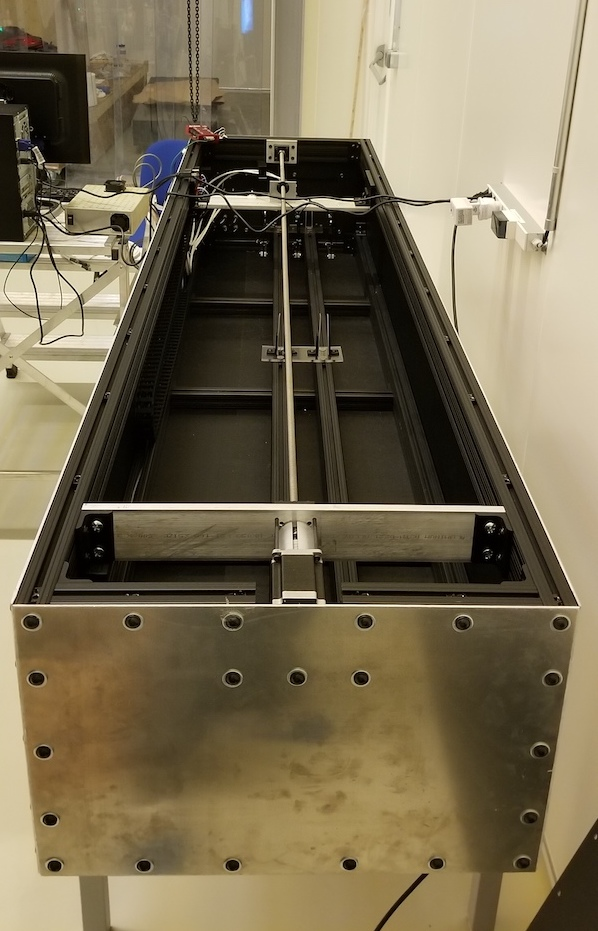
\includegraphics[height=.40\textheight, angle=0]{pds-scanner}
\end{dunefigure}

Access to the \dwords{pd} inside the \dword{apa}s is severely limited once the \dword{ce} cable conduit is in place, so identifying problems early in the process is necessary to minimize schedule issues caused by required \dword{pd} maintenance or repair due to problems detected during installation.

Following the optical scan, the \dword{pd} modules are inserted into an  \dword{apa} at the \dword{pd} integration area in the cleanroom. The connection to the cable harness, which is pre-installed in the \dword{apa} before wire wrapping, is automatic. An electrical continuity check follows insertion to verify  continuity between the \dword{pd} module and the \dword{pd} cable end connector at the end of the \dword{apa}.

\begin{comment}
Once integrated \dword{apa}s are received in the \dword{sas} for the cleanroom in front of the cryostat, an electrical connectivity test between the cable end exiting the \dword{apa} to be installed and each of the \dword{pd} modules in that \dword{apa} will be performed.  Discussions are underway with the \dword{apa} consortium to determine if the transport frames for shipping the integrated \dword{apa} pairs can be made sufficiently light-tight to allow biasing the photosensors and checking that they are operating properly.  Accessing the \dword{pd} modules involves removing the \dword{ce} cable conduits from the \dword{apa} side tubes, so this is the last time in the installation process that \dwords{pd} can be reached for repair or replacement.  Any repairs to the \dword{pd} system discovered later in the installation process would require returning the \dword{apa} module to this point in the installation sequence.
\end{comment}

As the upper and lower \dword{apa}s are joined on the assembly tower, \dword{pd} cables from the upper to the lower \dword{apa} will be connected, and at that time, continuity checks will be made.

Once the upper and lower \dword{apa}s are joined, the assembled unit will be moved into a \coldbox in front of the cryostat for final testing.  This is an opportunity to make a final low-temperature check of the complete \dword{pd} \dword{ce} and cabling chain before installation into the cryostat.  \dword{pd} \dword{fe} electronics boards will be used to read out the photon system during the cold test, and results will be compared to previous \dword{qa} test results.

The \dword{apa} stack is rolled into position in the cryostat following the \coldbox test, and the \dword{pd} and \dword{ce} cables connected to the cryostat flange.  At this point, a final continuity check is made from the flange bulkhead to the \dword{pd} module.

Discussions are underway with the installation team to arrange for a one-shift dark test of the installed \dwords{pd} in the cryostat following final installation, verifying end-to-end system operation.

\subsubsection{Calibration System Testing}
The laser system is aligned and tested as the lasers are installed. This requires an initial alignment with the alignment laser then testing with the UV laser under controlled conditions. Details of the testing procedures have not yet been developed. The pulsed neutron source will be calibrated off-line to verify the shielding design and neutron flux.  The source will be operated in test mode \textit{in situ} to verify the functionality. 

\begin{comment}
%%%%%%%%%%%%%%%%%%%%%%%%%%%%
\subsection{Environmental, Safety, and Health (ES\&H)}
\label{sec:fdsp-tc-inst-safety}

\fixme{check once the TC volume is done. Anne}
\dword{fnal} and \dword{dune} are committed to supporting the health and safety of staff, the community, and the environment in research and operations, as stated in the \dword{lbnf}/\dword{dune} Integrated Safety Management Plan\cite{bib:docdb291}. The safety and health program complies with applicable standards and local, state, and federal legal requirements through \dword{fnal}'s Work Smart Set of Standards \fixme{ref -ask Mike A} and the contract between \dword{fra} and the \dword{doe}. \dword{fnal} and the \dword{sdsd} have the host laboratory responsibilities for \dword{lbnf} and \dword{dune} operations at \dword{surf} in Lead, South Dakota.
The Fermilab facilities are further subject to the requirements of the \dword{doe} Workers Safety and Health Program 10 CFR 851\cite{doe-10cfr851}. These requirements are promulgated through the Fermilab Directors Policy Manual, and the \dword{feshm}, which align with the \dword{surf} \dword{esh} manual.

%While \dword{esh} will be  a host laboratory (Fermilab/SDSD) responsibility, a  Global Safety Coordination group will evaluate applicable codes and standards including international code equivalency for the design, assembly, and installation of the \dword{dune} detectors. The Global Safety Coordination group is  a team of engineering and \dword{esh} experts from within \dword{lbnf} and \dword{dune} organizations.  These requirements will be adopted by \dword{dune}, JPO (Joint Project Office), and \dword{lbnf} organizations and used to develop manufacturing, assembly, and installation processes and procedures. 
While \dword{esh} is  a host laboratory (\dword{fnal}'s \dword{sdsd}) responsibility, a  \dword{gsc} will evaluate applicable codes and standards including international code equivalency for the design, assembly, and installation of the \dword{dune} \dwords{detmodule}. The \dword{gsc} is  a team of engineering and \dword{esh} experts from within \dword{lbnf} and \dword{dune} organizations.  These requirements will be adopted by \dword{dune}, \dword{jpo}, and \dword{lbnf} organizations and used to develop manufacturing, assembly, and installation processes and procedures. 
\dword{dune} will develop an %Installation 
\dword{esh} plan for installation that will define %a specific set of 
the \dword{esh} requirements and responsibilities that personnel will be required to follow while  assembling, installing, and constructing equipment at \dword{surf}. % and \dword{itf}. 

{\bf Work Planning and Controls:} The goal of the work planning and \dword{ha} process is to initiate thought about the hazards associated with work activities and how the work can be performed safely. Careful planning of a job assures that it is performed efficiently and safely. Work planning ensures the scope of the job is understood, appropriate materials and tools are available, all hazards have been identified, mitigation efforts established, and all affected employees understand what is expected of them. %\dword{ha} is a critical part of work planning.  
The Work Planning and Hazard Analysis program is documented in Chapters 2060 in the \dword{feshm}.

The shift supervisor will lead %daily 
work planning meetings at the start of each shift to coordinate work activities, review hazards and mitigations, and answer any questions.

{\bf Documentation Approval Process:} The engineering review and approval process of all required documentation includes structural calculations, assembly drawings, load tests, \dwords{ha}, and procedural documents for \fixme{a set of identified?} typical individual tasks.  For the larger operations and systems like \dword{tpc} component factories, the \dword{dss}, cleanroom, and assembly infrastructure, this will be followed by an \dword{orr} by a joint safety committee that visits the site  after reviewing the documentation, and watches the full operation before signing off on the documentation.

{\bf \dword{esh} Support:} Safety starts from the ground up, both on the surface and in the underground facilities. All employees have work stop authority in support of  a safe working environment. Personnel will need to use the necessary \dword{ppe} identified through the \dword{ha} process for the task. A local \dword{esh} coordinator under the direction of the \dword{dune} \dword{esh} Manager will provide daily support for the facilities and attend the %daily 
\fixme{they are either daily or per shift - sounds like `per shift' is correct}
work planning meetings to notify each shift of potential safety issues and constraints, to ensure that  employees have the necessary \dword{esh} training, and to be responsible \fixme{to make sure the workers are responsible? or so that  the coordinator has what they need so that they can be responsible?} for managing \dword{esh} related  documentation including training records, weekly safety reports, near miss and accident reports, and equipment inspection.

{\bf Work Underground} \dword{sdsta} will maintain:
\begin{itemize}
    \item Site Access Control Program through \dwords{tap};
    \item \dword{em} program, which includes an Emergency Response incident command system and an \dword{ert}.  Typically, a small number of employees underground (guides) are also training as first responders to help in a medical emergency.
    
\end{itemize}

{\bf Equipment operation:} All overhead cranes, gantry cranes, fork lifts, motorized equipment trains/carts will be operated only by trained licensed operators. 
Other equipment, e.g., scissor lifts, pallet jacks, hand tools, and shop equipment, may only be operated by people trained
and certified for the particular piece of equipment.

{\bf House cleaning:} All workers underground are responsible for keeping a clean organized work area. Flammable items must be in proper storage cabinets, and items like empty shipping crates and boxes must be removed and %shipped 
transported back to the surface to make space.

{\bf \dword{ppe}:} 
\dword{ppe} is the responsibility of the host laboratory,  %(Fermilab/SDSD) and will be supplied 
which will supply it to all workers. 

{\bf Access and training:}  All \dword{dune} workers requiring access to the \dword{surf} site must (1) register through the \dword{fnal} Users Office to receive the necessary user training and a \dword{fnal} ID number, and they must apply for a \dword{surf} identification badge. % for \dword{dune} activities. 
All \dword{dune} workers will be required to complete \dword{surf} Surface and Underground Orientation classes. Workers accessing the underground must also complete 4850 and 4910 level specific unescorted access training. %A guide must be stationed on all working levels and have received the necessary guide training. 
A properly trained guide will be stationed on all working levels. 

{\bf Requirements at collaborating %laboratories and 
institutions:} All work performed at collaborating institutions will be completed in accordance with the %collaborating 
institution's \dword{esh} policies and programs. 
Equipment and operating procedures provided by the %collaborating 
institution must conform to the \dword{dune} Project \dword{ieshp}. %\dword{esh} and Integrated Safety Management policies and procedures. 
The %collaborating 
institution's \dword{esh} department is responsible for providing \dword{esh}  oversight for all work activities carried out in their facilities. % in collaborating institution facilities. 
\dword{lbnf} and \dword{dune} personnel will also follow the \dword{esh} manual and procedures of the collaborating institutions.

\end{comment}
